\documentclass[12pt]{article}
\setlength{\oddsidemargin}{-0.125in}
\setlength{\topmargin}{-0.5in} \setlength{\textwidth}{6.5in}
\setlength{\textheight}{9in}

\setlength{\textheight}{9in} \setlength{\textwidth}{6.5in}
\setlength{\topmargin}{-40pt} \setlength{\oddsidemargin}{0pt}
\setlength{\evensidemargin}{0pt}

\setlength{\textheight}{8.5in} \setlength{\textwidth}{6.5in}
\setlength{\topmargin}{-36pt} \setlength{\oddsidemargin}{0pt}
\setlength{\evensidemargin}{0pt} \tolerance=500
\renewcommand{\baselinestretch}{1.5}
%\input psfig.tex
\usepackage{amssymb}
\usepackage{amsmath}
\usepackage{latexsym}
\usepackage{array}
\usepackage{morefloats}
\usepackage{epsfig}
\usepackage{rotating}
\usepackage{graphicx}
\usepackage{subfigure}
\usepackage{url}
\usepackage{mathtools}
\usepackage{enumerate}
\usepackage{wasysym}
\usepackage{threeparttable}
\usepackage{lscape}
\usepackage{natbib}
\usepackage{color}
\usepackage{epstopdf}
\usepackage{hyperref}
\usepackage{bm, bbm}

% \usepackage{subfig,siunitx}
% \usepackage{dcolumn}
% \usepackage[margin=1cm]{caption}
% \newcolumntype{d}[1]{D{.}{.}{#1}}
%\usepackage{mathtools}

\newcommand{\mbv}[1]{\mbox{\boldmath$#1$\unboldmath}}
\newcommand{\mbf}[1]{\mathbf{#1}}
\newcommand{\iid}{\stackrel{\mathrm{iid}}{\sim}}
\newcommand{\mcal}[1]{\mathcal{#1}}
\newcommand{\bl}{\color{blue}}
\newcommand{\gr}{\color{green}}
\newcommand{\rd}{\color{red}}
\newcommand{\blk}{\color{black}}
\newcommand{\mbb}[1]{\mathbb{#1}}
\newtheorem{theorem}{Theorem}[section]
\newtheorem{lemma}[theorem]{Lemma}
\newtheorem{proposition}[theorem]{Proposition}
\newtheorem{corollary}[theorem]{Corollary}

\newenvironment{proof}[1][Proof]{\begin{trivlist}
\item[\hskip \labelsep {\bfseries #1}]}{\end{trivlist}}
\newenvironment{definition}[1][Definition]{\begin{trivlist}
\item[\hskip \labelsep {\bfseries #1}]}{\end{trivlist}}
\newenvironment{example}[1][Example]{\begin{trivlist}
\item[\hskip \labelsep {\bfseries #1}]}{\end{trivlist}}
\newenvironment{remark}[1][Remark]{\begin{trivlist}
\item[\hskip \labelsep {\bfseries #1}]}{\end{trivlist}}

\newcommand{\qed}{\nobreak \ifvmode \relax \else
      \ifdim\lastskip<1.5em \hskip-\lastskip
      \hskip1.5em plus0em minus0.5em \fi \nobreak
      \vrule height0.75em width0.5em depth0.25em\fi}

%%%%%%%%%%%%%%%%%%%%%%%%%%%%%%%%%%%%%%%%%%
\def\wt{\widetilde}
\def\diag{\hbox{diag}}
\def\wh{\widehat}
\def\AIC{\hbox{AIC}}
\def\BIC{\hbox{BIC}}
%- Makes the section title start with Appendix in the appendix environment
\newcommand{\Appendix}
{%\appendix
\def\thesection{Appendix~\Alph{section}}
%\def\thesubsection{\Alph{section}.\arabic{subsection}}
\def\thesubsection{A.\arabic{subsection}}
}
\def\diag{\hbox{diag}}
\def\log{\hbox{log}}
\def\bias{\hbox{bias}}
\def\Siuu{\boldSigma_{i,uu}}
\def\ANNALS{{\it Annals of Statistics}}
\def\BIOK{{\it Biometrika}}
\def\whT{\widehat{\Theta}}
\def\STATMED{{\it Statistics in Medicine}}
\def\STATSCI{{\it Statistical Science}}
\def\JSPI{{\it Journal of Statistical Planning \& Inference}}
\def\JRSSB{{\it Journal of the Royal Statistical Society, Series B}}
\def\BMCS{{\it Biometrics}}
\def\COMMS{{\it Communications in Statistics, Theory \& Methods}}
\def\JQT{{\it Journal of Quality Technology}}
\def\STIM{{\it Statistics in Medicine}}
\def\TECH{{\it Technometrics}}
\def\AJE{{\it American Journal of Epidemiology}}
\def\JASA{{\it Journal of the American Statistical Association}}
\def\CDA{{\it Computational Statistics \& Data Analysis}}
\def\dfrac#1#2{{\displaystyle{#1\over#2}}}
\def\VS{{\vskip 3mm\noindent}}
\def\boxit#1{\vbox{\hrule\hbox{\vrule\kern6pt
          \vbox{\kern6pt#1\kern6pt}\kern6pt\vrule}\hrule}}
\def\refhg{\hangindent=20pt\hangafter=1}
\def\refmark{\par\vskip 2mm\noindent\refhg}
\def\naive{\hbox{naive}}
\def\itemitem{\par\indent \hangindent2\parindent \textindent}
\def\var{\hbox{var}}
\def\cov{\hbox{cov}}
\def\corr{\hbox{corr}}
\def\trace{\hbox{trace}}
\def\refhg{\hangindent=20pt\hangafter=1}
\def\refmark{\par\vskip 2mm\noindent\refhg}
\def\Normal{\hbox{Normal}}
\def\povr{\buildrel p\over\longrightarrow}
\def\ccdot{{\bullet}}
\def\be{\begin{eqnarray}}
\def\ee{\end{eqnarray}}
\def\bq{\begin{equation}}
\def\eq{\end{equation}}
\def\bse{\begin{eqnarray*}}
\def\ese{\end{eqnarray*}}
\def\pr{\hbox{pr}}
\def\wh{\widehat}
\def\trans{^{\rm T}}
\def\myalpha{{\cal A}}
\def\th{^{th}}
\def\bs{\mathbf{s}}

\DeclarePairedDelimiter\ceil{\lceil}{\rceil}
\DeclarePairedDelimiter\floor{\lfloor}{\rfloor}


% \newcommand\independent{\protect\mathpalette{\protect\independenT}{\perp}}
% \def\independenT#1#2{\mathrel{\rlap{$#1#2$}\mker2mu{#1#2}}}
% \DeclareMathOperator{\E}{E}
% \DeclareMathOperator{\V}{V}
\DeclareMathOperator{\vect}{vec}
\DeclareMathOperator{\vech}{vech}
%\DeclareMathOperator{\diag}{diag}

% \newtheoremstyle{break}
%   {\topsep}{\topsep}%
%   {\itshape}{}%
%   {\bfseries}{}%
%   {\newline}{}%
% \theoremstyle{break}

\newtheorem{alg}{Algorithm}

\begin{document}
\thispagestyle{empty} \baselineskip=28pt

\begin{center}
%{\LARGE{\bf Particle Swarm Optimization Assisted Metropolis Hastings Algorithms}}
{\LARGE{\bf Particle Swarm Optimization Assisted Metropolis Hastings Algorithms}}
\end{center}

\baselineskip=12pt
%%
\vskip 2mm
\begin{center}
Matthew Simpson\footnote{(\baselineskip=10pt to whom correspondence should be addressed)
Department of Statistics, University of Missouri,
146 Middlebush Hall, Columbia, MO 65211-6100, themattsimpson@gmail.com}
%Matthew Simpson,\footnote{(\baselineskip=10pt to whom correspondence should be addressed)
%Department of Statistics, University of Missouri,
%146 Middlebush Hall, Columbia, MO 65211-6100, themattsimpson@gmail.com}
% Christopher K. Wikle,\footnote{\label{note:aff}\baselineskip=10pt
% Department of Statistics, University of Missouri,
% 146 Middlebush Hall, Columbia, MO 65211-6100}
% and Scott H. Holan\textsuperscript{\ref{note:aff}}
\end{center}

\vskip 2mm
\begin{center}
{\large{\bf Abstract}}
\end{center}
Fitting dependent data models is a challenging endeavor and often requires some form of dimension reduction or customized estimation algorithm. Particle swarm optimization (PSO) refers to a class of heuristic optimization algorithms that exploit analogies with animal flocking behavior in order to obtain optima without strong conditions on the objective function. We introduce two new classes of PSO algorithms based, termed adaptively tuned PSO (AT-PSO), and adaptively tuned bare bones PSO (AT-BBPSO). In both algorithms we add a dynamically tuned parameter to previously existing PSO algorithms. We propose using these PSO algorithms to approximate Bayesian posterior distributions in order to construct efficient proposals for independent Metropolis-Hastings algorithms. In order to illustrate our method and compare it to alternatives, we provide a simulation study and apply it to constructing a Markov chain Monte Carlo (MCMC) algorithm to estimate a reduced rank spatial model of county American Community Survey (ACS) 5-year estimates of county populations in the United States.
\baselineskip=12pt 

\baselineskip=12pt
\par\vfill\noindent
{\bf KEY WORDS:} 
Bayesian estimation; Markov chain Monte Carlo; Official statistics; Optimization; Spatial data
\par\medskip\noindent


\clearpage\pagebreak\newpage \pagenumbering{arabic}
\baselineskip=24pt

\section{Introduction}

[REWRITE THIS PARAGRAPH - IS TALL DATA WORTH MENTIONING?]
One common type of big data problem may be called ``tall'' data --- that is many observations of a relatively small number of variables. Bayesian estimation of tall data models can be particularly challenging in the dependent data and non-Gaussian settings due to the need to estimate or integrate out a high dimensional latent process, e.g., with dimension equal to the size of the dataset. Sometimes the latent process can be written as a function of a relatively small number of latent random variables, but, even in this case, standard Markov chain Monte Carlo (MCMC) techniques to approximate the posterior are often still slow. A common alternative is to leverage normal approximations to the posterior to obtain approximations to the marginal distributions of each parameter, e.g., INLA \citep{rue2009approximate}. This is approximation is often very good and much faster than MCMC, though neither advantage is universally true, particularly when features of the joint posterior distribution rather than just the marginals are desired or when the parameter space is too large (e.g., see \citet{taylor2014inla}). [CHECK ON THE JOINT VS MARGINAL THING AND OTHER INLA LIMITATIONS --- CITATIONS!!!] Another common strategy is to use Hamiltonian Monte Carlo (HMC) \citep{neal2011mcmc}, particularly the No-U-Turn sampler (NUTS) \citep{homan2014no} which is implemented in the Stan software \citep{carpenter2015stan}. However HMC requires many log posterior evaluations per iteration and in the tall data setting these are typically expensive.

We propose using old MCMC technology improved by new optimization techniques. It is well known that a Bayesian posterior distributions for a fixed set of parameters tends asymptotically to a normal distribution centered at the posterior mode as the sample size increases; see \citet[Chapter~7.4]{schervish1997theory}. This normal approximation, often called a Laplace approximation, is used by INLA but is also frequently used to construct independent Metropolis-Hastings (IMH) samplers \citep{metropolis1953equation,hastings1970monte} --- typically using a $t$ proposal instead of a normal. IMH samplers based on a good approximation to the posterior distribution typically have high acceptance rates along with fast mixing and convergence, but it is often impractical to find an adequate approximation. Even in cases where the normal approximation is appropriate the posterior may be too high dimensional for this approach to be practical. In larger models numerical methods are usually required to find the posterior mode and sometimes also to integrate out a latent process, but standard methods for doing so are usually prohibitively slow or fail outright. However, new heuristic optimization algorithms tend to work reasonably well over a wider class of objective functions and in larger parameter spaces, for example, genetic algorithms \citep{goldberg1988genetic} and particle swarm optimization (PSO) \citep{clerc2002particle,blum2008swarm,clerc2010particle}. We propose using PSO to obtain the posterior mode so that effective independent Metropolis samplers can be constructed in a wider range of models. Other heuristic optimization algorithms may be useful for the same task, but we do not explore them here. We also develop several novel PSO algorithms that help obtain good estimates of the posterior mode and that may also have utility in other optimization contexts. We illustrate our method on two different modeling applications. The first application considers a group of reduced rank spatial models of American Community Survey (ACS) 5-year period estimates of county population estimates for the U.S. in 2014. In the second application, we adapt a hierarchical model for predicting the outcome of the 1988 presidential election from \citet{gelman2006data}. We fit these models using our proposed independent Metropolis-Hastings algorithm, an independent Metropolis within Gibbs algorithm based on the same Laplace approximation, and a variety of other MCMC algorithms. We compare the computational cost for each of the algorithms and discuss their ease of use. 

[REWRITE THIS PARAGRAPH - SECTIONS HAVE CHANGED]
The remainder of this paper is organized as follows. Section~\ref{sec:pso} introduces PSO along with our novel PSO algorithms and reports the results of testings these algorithms on a suite of standard test functions. Section~\ref{sec:psometrop} describes the IMH algorithms we construct with the aid of PSO whereas Section~\ref{sec:glm} describes a general strategy for using our method to fit generalized linear mixed models and details our applications. Section~\ref{sec:compest} compares our MCMC techniques to a variety of other techniques for our applications, and Section~\ref{sec:discuss} concludes with discussion. 



\section{Particle swarm optimization}\label{sec:pso}
We briefly describe PSO here; refer to \citet{blum2008swarm} for an excellent introduction and \citet{clerc2010particle} for more detail. Suppose that we wish to optimize some objective function $Q(\bm{\theta}):\Re^D\to\Re$ --- without loss of generality we will assume the goal is maximization. Let $i=1,2,\dots,n$ index a set of particles over time, $t=1,2,\dots,T$, where each particle consists of a location at every period $\bm{\theta}_i(t)\in \Re^D$, a velocity $\bm{v}_i(t) \in \Re^D$, a personal best location $\bm{p}_i(t)\in\Re^D$, and a group best location $\bm{g}_i(t)\in\Re^D$. Here we mean ``best'' in the sense of maximizing $Q$, so the objective function evaluated at $\bm{p}_i(t)$ is larger than at any point in particle $i$'s history. More formally $Q(\bm{p}_i(t)) \geq Q(\bm{\theta}_i(s))$ for any $s\leq t$. The group best location is defined with respect to some neighborhood $\mathcal{N}_i$ of particle $i$; that is, $\bm{g}_i(t) = \arg\max_{\{\bm{p}_j|j\in\mathcal{N}_i\}}Q(\bm{p}_j(t))$. In the simplest case where the entire swarm is the neighborhood of each particle, $\bm{g}_i(t)\equiv \bm{g}(t) = \arg\max_{j\in 1:n}Q(\bm{p}_j(t))$. The generic PSO algorithm updates as follows:
\begin{align}\label{eq:pso}
\bm{v}_i(t+1) &= \omega \bm{v}_i(t) + \phi_1 \bm{r}_{1i}(t)\circ\{\bm{p}_i(t) - \bm{\theta}_i(t)\} + \phi_2 \bm{r}_{2i}(t)\circ\{\bm{g}_i(t) - \bm{\theta}_i(t)\},\nonumber\\
\bm{\theta}_i(t+1) &= \bm{\theta}_i(t) + \bm{v}_i(t+1),\nonumber\\
\bm{p}_i(t+1) &= \begin{cases} \bm{p}_i(t)   & \mbox{if }\  Q(\bm{p}_i(t)) \ge Q(\bm{\theta}_i(t + 1))\\
                               \bm{\theta}_i(t+1) & \mbox{otherwise},
\end{cases}\nonumber\\
\bm{g}_i(t+1) &= \arg\max_{\{\bm{p}_j(t+1)|j\in\mathcal{N}_i\}}Q(\bm{p}_j(t+1)),
\end{align}
where $\circ$ denotes the Hadamard product (element-wise product), $\bm{r}_{1i}(t)$ and $\bm{r}_{2i}(t)$ are each vectors of $D$ random variates independently generated from the $U(0,1)$ distribution, and $\omega>0$, $\phi_1>0$, and $\phi_2>0$ are user-defined parameters. The term $\omega \bm{v}_i(t)$ controls the particle's tendency to keep moving in the direction it is already going, so $\omega$ is called the inertia parameter. For $\omega<1$ velocities tend to decrease over time, while for $\omega>1$ they tend to increase over time. Similarly $\phi_1 \bm{r}_{1i}(t)\circ(\bm{p}_i(t) - \bm{\theta}_i(t))$ controls the particle's tendency to move towards its personal best location while $\phi_2 \bm{r}_{2i}(t)\circ(\bm{g}_i(t) - \bm{\theta}_i(t))$ controls its tendency to move toward the group's best location, so $\phi_1$ and $\phi_2$ are called the cognitive correction factor and social correction factor, respectively \citep{blum2008swarm}. This version of PSO is equivalent to \citet{clerc2002particle}'s constriction type I particle swarm. There are many variants of the PSO algorithm, often obtained through defining neighborhoods using different neighborhood topologies or choosing $(\omega,\phi_1,\phi_2)$ in special ways or sometimes even dynamically. A default version of the algorithm sets $\omega = 0.7298$ and $\phi_1 = \phi_2 = 1.496$; see \citet{clerc2002particle} and \citet{blum2008swarm} for justification of these choices. One advantage to these parameter values is that there are good theoretical reasons that something known as velocity clamping is unnecessary, though in some applications it may still be improve the algorithm. Even when $\omega<1$, if $\phi_1$ and $\phi_2$ are set high enough the velocities of the particles can continually increase and cause the swarm to make jumps that are much too large. Velocity clamping restricts this by setting an upper bound on the velocity of any particle in any given direction, though the default parameter values suggested by \citet{clerc2002particle} are also designed to prevent this sort of velocity explosion.

Any PSO variant can also be combined with various neighborhood topologies that control how the particles communicate to each other. The global topology allows each particle to see each other particle's previous best location, but this can cause inadequate exploration and premature convergence. Appendix \ref{sec:psocompare} contains a short description of the ring topologies, which we employ as a method of restricting information flow across the swarm in order to ameliorate these problems, but there are many alternatives in the literature.[CITATION]

Even in the simplest case, one downside of PSO is that both $\phi_1$ and $\phi_2$ need to be specified by the user, though there are some reasonable default choices. The bare bones PSO algorithm (BBPSO) is a PSO algorithm introduced by \citet{kennedy2003bare} that strips away the velocity term for simplification and removes the need for the user to choose parameters outside of the swarm size. Let $\theta_{ij}(t)$ denote the $j$th coordinate of the position for the $i$th particle in period $t$, and similarly for $p_{ij}(t)$ and $g_{ij}(t)$. Then the BBPSO algorithm obtains a new position coordinate $\theta_{ij}$ via
\begin{align}\label{eq:bbpso}
\theta_{ij}(t+1) \sim N\left(\frac{p_{ij}(t) + g_{ij}(t)}{2}, |p_{ij}(t) - g_{ij}(t)|^2\right)
\end{align}
where $N(\mu,\sigma^2)$ is the normal distribution with mean $\mu$ and standard deviation $\sigma^2$. The updates of $\bm{p}_i(t)$ and $\bm{g}_i(t)$ are the same as in \eqref{eq:pso}. There are several variants of this algorithm proposed including using distributions from different location-scale families --- e.g., using the $t$-distribution and modifying the location or the scale parameters (for example \citet{krohling2009bare}, \citet{hsieh2010modified}, \citet{richer2006levy}, and \citet{campos2014bare}). A commonly used variant of BBPSO also introduced by \citet{kennedy2003bare}, sometimes called BBPSOxp, gives each coordinate of $\bm{\theta}_i(t+1)$ a $0.5$ probability of moving to its group best location on that coordinate; i.e.,
\begin{align*}
\theta_{ij}(t+1) = \begin{cases} N\left(\frac{p_{ij}(t) + g_{ij}(t)}{2}, |p_{ij}(t) - g_{ij}(t)|^2\right) & \mbox{with probability }0.5\\
g_{ij}(t) &\mbox{otherwise}.\end{cases}
\end{align*}
This specification tends to bias the algorithm toward local optima and may not be ideal for multimodal objective functions, but it does accelerate convergence for more well behaved objective functions. 

A downside of both versions of BBPSO above is that any particle currently at its group best location does not move due to the definition of the standard deviation term. Several methods have been proposed to overcome this; e.g., see \citet{hsieh2010modified} and \citet{zhang2011novel}. \citet{zhang2011novel} propose using mutation and crossover operations for the group best particle. To do this, the group best particle randomly selects three other distinct particles $i_1$, $i_2$, and $i_3$, and updates:
\begin{align}\label{eq:bbpsomc}
\theta_{ij}(t+1) = p_{i_1j}(t) + 0.5(p_{i_2j}(t) - p_{i_3j}(t)).
\end{align}
When combined with BBPSOxp, this becomes
\begin{align}\label{eq:bbpsoxpmcbest}
\theta_{ij}(t+1) = \begin{cases} p_{i_1j}(t) + 0.5(p_{i_2j}(t) - p_{i_3j}(t)) & \mbox{with probability }0.5\\
g_{ij}(t) &\mbox{otherwise,}\end{cases}
\end{align}
but it also introduces another problem --- a particle which moves to its group best location on a single coordinate will have a standard deviation of zero for that coordinate during the next iteration. This is easily overcome by manually setting the standard deviation to a small value (e.g., 0.001), which allows us to define the two base BBPSO algorithms that we will consider: BBPSO-MC and BBPSOxp-MC. BBPSO-MC is standard BBPSO where each particle evolves according to \eqref{eq:bbpso} except any current group best particle evolves according to \eqref{eq:bbpsomc}. BBPSOxp-MC evolves every particle according to 
\begin{align}\label{eq:bbpsoxpmcall}
\theta_{ij}(t+1) = \begin{cases} N\left(\frac{p_{ij}(t) + g_{ij}(t)}{2}, \sigma^2_{ij}(t)\right) & \mbox{with probability }0.5\\
g_{ij}(t) &\mbox{otherwise,}\end{cases}
\end{align}
where $\sigma_{ij}(t) = |p_{ij}(t) - g_{ij}(t)|$ if $|p_{ij}(t) - g_{ij}(t)|>0$ and $\sigma_{ij}(t) = 0.001$ otherwise, except current group best particles evolve according to \eqref{eq:bbpsoxpmcbest}. 

\subsection{Adaptively tuned BBPSO}\label{subsec:ATBBPSO}
\citet{hsieh2010modified} propose a modified version of BBPSO with 
\begin{align*}
\theta_{ij}(t+1) \sim N\left(\omega_1\frac{p_{ij}(t) + g_{ij}(t)}{2}, \omega_2|p_{ij}(t) - g_{ij}(t)|^2\right),
\end{align*}
where $\omega_1$ and $\omega_2$ are constriction parameters that are eventually both set to one after enough iterations of the algorithm. The authors suggest dynamically adjusting the constriction parameters in the early stage of the algorithm before they are set to one, but give no suggestion for how to do this. We propose a variant of this algorithm where $\omega_1=1$ and where $\omega_2\equiv\sigma$ is a dynamically adjusted scale parameter, and additionally we propose using a more general student's $t$-distribution. Given a value for $\sigma(t)$ in period $t$, $\theta_{ij}(t+1)$ is obtained via
\begin{align}\label{eq:at-bbpso}
\theta_{ij}(t+1) \sim T_{df}\left(\frac{p_{ij}(t) + g_{ij}(t)}{2}, \sigma(t)|p_{ij}(t) - g_{ij}(t)|^2\right)
\end{align}
where $df$ is a degrees of freedom parameter. Define the improvement rate of the swarm in period $t$ as $R(t) = \#[\{i:Q(\bm{p}_i(t))> Q(\bm{p}_i(t-1))\}]/n$, where if $A$ is a set then $\#(A)$ is the number of members of that set. Heuristically, we can think about this rate similar to a random walk Metropolis acceptance rate. If the rate is too large, the jumps we are proposing are too small; so, while each particle is likely to find a new best location, the improvement will tend to be small. Similarly, if the rate is too small the jumps are too large and very few improvements occur. 

%This analogy is not quite right, however. For example imagine $\sigma=0$ so that $\theta_{ij}(t+1) = (p_{ij}(t) + g_{ij}(t))/2$ deterministically. The analogy suggests that each iteration will result in an improvement in the personal bests for the entire swarm. This is true so long as the objective function is strictly quasiconcave; i.e., upper contour sets of the objective function are strictly convex. An objective function with multiple local maxima is an easy counterexample. However, keeping the quasiconcave case in mind imagine a line drawn through a given particle's personal best $\bm{p}_i$ and the group best $\bm{g}_i$. The center of the movement distribution, $(\bm{p}_i + \bm{g}_i)/2$, is halfway between $\bm{p}_i$ and $\bm{g}_i$ on this line. As $\sigma$ increases, the probability that the new position is an improvement over the particle's previous best decreases because it increases the probability of the new location landing {\it behind} $\bm{p}_i$ instead of {\it between} $\bm{p}_i$ and $\bm{g}_i$. Howevewer, it also increases the probability of jumping {\it past} $\bm{g}_i$, which will tend to increase the size of the improvements in the particle's personal best when they do happen. Thus there is a trade-off between the improvement rate and the size of improvements. [MAKE A GRAPHIC FOR THIS AND/OR EXPLAIN IT BETTER OR CUT IT]

%While the above is heuristic and strictly speaking only applies to quasiconcave objective functions, we may nonetheless use it as a guide and think about setting and tuning $\sigma$. In particular,

The rates we observe will depend on particular parameter values we choose for the algorithm, but using the above intuition we can automatically and adaptively tune the scale parameter. Let $\lambda(t) = \log \sigma(t)$ and $R^*$ denote the target improvement rate. Then we update $\lambda(t)$ to $\lambda(t+1)$ each iteration via $\lambda(t+1) = \lambda(t) + c\times sgn(R(t) - R^*)$ where 
\begin{align*}
sgn(x) = \begin{cases} \phantom{-}1 & \mathrm{ if  }\ \ x > 0\\
                       \phantom{-}0 & \mathrm{ if  }\ \ x = 0\\
                                - 1 & \mathrm{ if  }\ \ x < 0\end{cases}
\end{align*}
and $c$ is some user-defined constant, e.g., $c=0.1$. Call BBPSO algorithms which use this adaptively tuned BBPSO (AT-BBPSO --- e.g., AT-BBPSO-MC and AT-BBPSOxp-MC). One nice feature of this algorithm is that it tunes the effective search space adaptively as the algorithm gets closer to the optimum. To some degree this already occurs with the $|p_{ij} - g_{ij}|$ term in the standard deviation. However, once BBPSO has approximately converged a more targeted local search may still yield improvement. AT-BBPSO increases the number of user-defined parameters relative to BBPSO, but they are fairly easy to select. These parameters are $\lambda(0)$, $c$, swarm size, $R^*$, and the degrees of freedom of the $t$-distribution. The value of $\lambda(0)$ has little effect on the algorithm since it adapts fairly quickly, so the user can safely leave it at a default value. We set $\lambda(0)=0$ since that initializes the AT-BBPSO algorithm at an equivalent BBPSO algorithm. The value of $c$ has a slightly higher impact, but again it is relatively small. It controls how fast $\lambda(t)$ adapts and how precisely it can adapt. A larger value of $c$ causes $\lambda(t)$ to adapt more quickly, but it also means that the set of possible values that $\lambda(t)$ can take on is smaller. Since $\lambda(t)$ can only take on values on the the lattice $\{\dots, \lambda(0) - 2c, \lambda(0) - c, \lambda(0), \lambda(0) + c, \lambda(0) + 2c, \dots\}$, a larger value of $c$ makes it more likely that $\lambda(t)$ cannot get close to the value which yields the target improvement rate, which can cause the swarm to move toward the maximum more slowly. Optimizing this parameter can improve the algorithm, but in practice we find that the gains are small compared to just setting $c=0.1$.

The swarm size is a more difficult parameter to choose, though all PSO algorithms share it in common. The basic tradeoff is the classic accuracy versus speed tradeoff. A larger swarm size yields better estimates of the maximum but at the cost of more function evaluations. To some extent increasing the swarm size is a substitute for running the algorithm for more iterations, though the number of iterations should typically be at least an order of magnitude larger than the swarm size. The consequential parameters of the AT-BBPSO algorithms are $R^*$ and $df$. The value of $R^*$ should be fairly small so that the algorithm can more easily jump between local maxima, yet large enough that it can converge on the global maximum once in its region. In our experience setting $R^*$ from  $0.3$ to $0.5$ tends to yield algorithms which do the best job of finding the global max, but since $R(t)$ can only take on values in a discrete set $R^*$ should also be set in concert with the size of the swarm. For example, if there are only 100 members of the swarm, then $R(t)$ can only take on the values $0/100, 1/100, 2/100, \dots, 100/100$ so setting $R^*=0.015$ or $R^*=0.019$ will result in the same behavior. The degrees of freedom parameter also should typically be set fairly small, e.g., $df=1$. Tinkering with these parameters is more likely to yield substantial improvements than with other parameters of the AT-BBPSO algorithms, though this is not always the case. Appendix \ref{sec:psocompare} justifies these choices in an extended simulation study on several test functions.

In the AT-BBPSOxp variants, the improvement rate is in a certain sense poorly targeted --- the rate is used to tune $\sigma(t)$ in \eqref{eq:at-bbpso}, but 50\% of the time $\theta_{ij}(t+1)$ will be set to $g_{ij}(t)$. So when $\bm{\theta}_i$ moves to a new personal best location, this may be because $\sigma(t)$ was set appropriately, or because it was forced to move to $\bm{g}_i$'s coordinate on several dimensions, or both. Despite this, tuning $\sigma(t)$ in the fashion described above still seems to perform well, which can be seen in Appendix \ref{sec:psocompare}.

\subsection{Adaptively tuned PSO}\label{sec:AT-PSO}
In AT-BBPSO variants, the parameter $\sigma(t)$ partially controls the effective size of the swarm's search area, and we increase or decrease $\sigma(t)$ and consequently the search area depending on how much of the swarm is finding new personal best locations. In standard PSO there is no direct analogue to $\sigma(t)$, though the inertia parameter, $\omega$ in \eqref{eq:pso}, is related. It controls the effective size of the swarm's search area by controlling how the magnitude of the velocities evolve over time --- larger values of $\omega(t)$ allow for larger magnitude velocities in future periods. In AT-BBPSO we use an analogy with tuning a random walk Metropolis-Hastings MCMC algorithm in order to build intuition about how to tune $\sigma(t)$. The analogy is much weaker in this case; nonetheless, we allow $\omega(t)$ to be time-varying and use the same mechanism in order to tune it as we did for $\sigma(t)$.

The idea of time-varying $\omega(t)$ has been in the PSO literature for some time. An early suggestion was to set $\omega(0)=0.9$ and deterministically decrease it until it reaches $\omega(T)=0.4$ after the maximum number of iterations allowed \citep{eberhart2000comparing}. In particular, \citet{tuppadung2011comparing} suggest defining $\omega(t)$ via the parameterized inertia weight function
\begin{align}\label{eq:inertiafun}
\omega(t) = \frac{1}{1 + \left(\frac{t}{\alpha}\right)^{\beta}}
\end{align}
where $\alpha$ and $\beta$ are user-defined parameters. Roughly, $\alpha$ controls how low $\omega(t)$ can go and $\beta$ controls how fast it gets there, so $\alpha$ and $\beta$ can be thought of as intercept and slope parameters respectively. The suggestion in \citet{tuppadung2011comparing} is to set $\alpha$ to a small fraction of the total amount of iterations in which the algorithm is allowed to run (e.g., 10\% or 20\%), and set $\beta$ between one and four.

This approach tends to improve on standard PSO if $\omega(t)$'s progression is set appropriately, but it invariably makes using PSO more difficult for the average user. Using a parameterized inertia weight function such as \eqref{eq:inertiafun} solves this somewhat, but it still introduces new parameters that must be chosen by the user. Depending on the problem, it may be more useful to let the swarm explore the space for more iterations, necessitating higher values of $\omega(t)$ for longer, or it may be more useful to let the swarm quickly move toward high value areas, necessitating lower values for $\omega(t)$ earlier. A priori it may not be clear exactly which approach is best for any given problem, so an automatic method is desirable. Adaptively tuned PSO (AT-PSO) is just that --- it provides an automatic method to adjust the value of $\omega(t)$ depending on local information obtained by the particle swarm. Formally, the AT-PSO updating equations are as follows:
\begin{align}\label{eq:atpso}
\log\omega(t+1)& = \log\omega(t) + c\times sgn(R(t) - R^*),\nonumber\\
\bm{v}_i(t+1) &= \omega(t+1) \bm{v}_i(t) + \phi_1 \bm{r}_{1i}(t)\circ\{\bm{p}_i(t) - \bm{\theta}_i(t)\} + \phi_2 \bm{r}_{2i}(t)\circ\{\bm{g}_i(t) - \bm{\theta}_i(t)\},\nonumber\\
\bm{\theta}_i(t+1) &= \bm{\theta}_i(t) + \bm{v}_i(t+1),\nonumber\\
\bm{p}_i(t+1) &= \begin{cases} \bm{p}_i(t)   & \mbox{if }\  Q(\bm{p}_i(t)) \ge Q(\bm{\theta}_i(t + 1))\\
                               \bm{\theta}_i(t+1) & \mbox{otherwise},
\end{cases}\nonumber\\
\bm{g}_i(t+1) &= \arg\max_{\{\bm{p}_j(t+1)|j\in\mathcal{N}_i\}}Q(\bm{p}_j(t+1))
\end{align}
where $R(t)$ is the improvement rate of the swarm in iteration $t$, $R^*$ is the target improvement rate, and $c$ controls how much $R(t)$ changes on a per iteration basis. For AT-BBPSO we used an analogy with random walk Metropolis-Hastings algorithms to suggest that a good value for the target improvement rate is smaller than 0.5 but not too small, and simulations in Appendix \ref{sec:psocompare} corroborate this and suggests that $R^*=0.3$ or $0.5$ are good values in many problems. The analogy does not apply so cleanly here though we find in Appendix \ref{sec:psocompare} that $R^*=0.3$ or $0.5$ still seems to work well for AT-PSO. In Appendix \ref{sec:psocompare} we speculate that lower values of $c$ will result in higher inertias for longer, and as a result improve AT-PSO algorithms when more initial exploration of the search space is desirable. We use $c=0.1$ as a default value, but in simulations (not reported here) we find that the gains from optimizing $c$ appear to be small, though a very small or very large value can cause the algorithm to perform poorly.

A major strength of AT-PSO is that, unlike DI-PSO, it can increase $\omega(t)$ when information from the swarm suggests there is an unexplored high value region of the space --- when too much of the swarm is improving on their personal best locations AT-PSO increases $\omega(t)$ until velocities start increasing, the swarm starts exploring a larger amount of the nearby space, and more of the particles fail to find improvements on their personal best. This mechanism provides a way for the swarm to adapt its behavior on the fly to the local conditions, though like many other methods of improving PSO algorithms, it may cause premature convergence in multimodal problems.

Appendix \ref{sec:psocompare} contains an extended simulation study comparing a variety of these PSO and BBPSO algorithms on a suite of test functions and motivates the following recommendations. When the goal is convergence, AT-PSO with $R^*=0.3$ or $0.5$ and ring-1 or ring-3 neighborhoods tends to work the best, though in problems where convergence is difficult AT-BBPSOxp with $R^*=0.3$ or $0.5$ and ring-1 or ring-3 neighborhoods will often find better evaluations of the objective function while they and alternative PSO algorithms fail to converge. This feature of AT-PSO suggests a hybrid strategy using a Stage 1 optimization algorithm to get close to the global optimum, then using AT-PSO in Stage 2 in order to obtain convergence. We explore this strategy in Section~\ref{sec:psomode} for several PSO algorithms in two statistical examples where the goal is to find the posterior mode for the Laplace approximation to the posterior. There we use the Broyden-Fletcher-Goldfarb-Shannon (BFGS) algorithm in Stage 1.




\section{PSO Assisted Independent Metropolis-Hastings}\label{sec:psometrop}
Next we turn to using PSO algorithms to help construct MCMC algorithms for sampling from a posterior distribution. Let $\bm{\theta}$ be the model parameter and $ p(\bm{\theta}|\bm{y}_{1:n})$ be its posterior distribution, available up to a normalizing constant. Further let $\bm{\theta}^*_n$ denote the posterior mode of $p(\bm{\theta}|\bm{y}_{1:n})$ and let $\bm{H}_n(\bm{\theta}^*_n)$ denote the Hessian matrix of $\log p(\bm{\theta}|\bm{y}_{1:n})$ evaluated at $\bm{\theta}_n^*$. Then under suitable regularity conditions \citep[Sections~7.4.2~and~7.4.3]{schervish1997theory} $\bm{\theta}$'s posterior distribution is asymptotically normal. So, for a fixed but large value of $n$, $\bm{\theta}|\bm{y}_{1:n} \stackrel{a}{\sim} N(\bm{\theta}_n^*, -\bm{H}_n^{-1}(\bm{\theta}^*_n))$ where the notation $\stackrel{a}{\sim}$ means ``approximately distributed as.''

The Laplace approximation to the posterior can be used to create a proposal distribution for an independent Metropolis MCMC algorithm, though a multivariate $t$-distribution is usually substituted for the normal so that the proposal has fatter tails than the target posterior.  Finding the posterior mode in closed form is typically impossible and standard numerical optimization algorithms perform poorly in high dimensional parameter spaces, but PSO can perform well in larger spaces. We use PSO to find the posterior mode, but other heuristic algorithms such as genetic algorithms \citep{goldberg1988genetic} could also be used. Additionally, for independent Metropolis algorithms it is not important that we find the true posterior mode; what is important is that we are close enough that the resulting Metropolis algorithm has a high acceptance rate. However, as we shall see in Section~\ref{sec:psomode}, sometimes when the estimate is slightly off the mode the algorithm will still have a poor acceptance rate. 

This sort of algorithm is more likely to be useful in the tall data setting, i.e. when the number of observations is large and much larger than the number of covariates, because the normal approximation should be fairly good and there is a reduced likelihood of an ill-behaved posterior density, e.g., a bimodal posterior distribution. Some parameters have no observations directly related to them, but instead define the distribution of some latent process. For these parameters it is crucial that there are enough realizations of the latent process in the model to ensure that the normal approximation works well for the higher level parameter. More formally, suppose the model can be written as $L(\bm{\theta},\bm{\psi}|\bm{y}_{1:n}) = \prod_{i=1}^np(\bm{y}_i|\bm{\psi}) \times p(\bm{\psi}|\bm{\theta})$. Here $\bm{y}_i$ may include response variables and covariates, $\bm{\psi}$ may include data model parameters and a latent process, and $\bm{\theta}$ includes all higher level parameters. As long as $n$ is large and the dimension of $\bm{\psi}$ is small, the normal approximation should work well for $\bm{\psi}$. In order for the normal approximation to work well for $\bm{\theta}$ as well, the elements of $\bm{\psi}$ need to depend on $\bm{\theta}$ in such a way that borrows strength across elements of $\bm{\psi}$. For example $p(\bm{\psi}|\bm{\theta}) = \prod_{j=1}^mp(\psi_j|\bm{\theta})$ where $m$ is larger than the dimension of $\bm{\theta}$. Many common models fit into this framework, for example, generalized linear mixed effect models where the number of random effects is relatively small and constant in the sample size and the covariance matrix of the random effects is a function of a low dimensional parameter. Some examples of these types of models are provided in Section~\ref{sec:glm}. While, strictly speaking, these are not necessary nor sufficient conditions for a PSO assisted Metropolis-Hastings algorithm to work well, they do serve as useful guidelines. For example, when the covariance matrix of the random effect vector in a generalized linear mixed model is fully parameterized we essentially have one observation to estimate it --- the estimate of the full random effect vector. As a result, the normal approximation is very poor and as we demonstrate in Section~\ref{sec:compest}, the resulting independent Metropolis-Hastings algorithm has poor acceptance rates. In some models analytically finding the Hessian may be complicated, but unfortunately this is necessary in higher dimensions because numerical methods to evaluate the Hessian will often fail or be prohibitively slow. The independent Metropolis-Hastings algorithm we use is standard and given by Algorithm~\ref{alg:IM1}:
\begin{alg}[Independent Metropolis-Hastings with Laplace approximation]\label{alg:IM1}
Given a user-chosen degrees of freedom parameter $df$, an estimate of the posterior mode $\bm{\theta}^*$ and the Hessian $\bm{H}^* \equiv \bm{H}(\bm{\theta}^*)$ with $\ell^* = \log p(\bm{\theta}^*|\bm{y}_{1:n})$ and $\bm{\Sigma}^* = (-\bm{H}^*)^{-1}$, obtain $\bm{\theta}^{(t+1)}$ from $\bm{\theta}^{(t)}$ via:
\begin{enumerate}
\item Draw proposal $\bm{\theta}^{(prop)} \sim T_{df}(\bm{\theta}^*, \bm{\Sigma}^*)$.
\item Compute the log posterior $\ell^{(prop)} = \log p(\bm{\theta}^{(prop)}|\bm{y}_{1:n})$.
\item Compute the log acceptance ratio 
\begin{align*}
\log a = \ell^{(prop)} - \ell^{(t)} + \log t_{df}(\bm{\theta}^{(t)}; \bm{\theta}^*, \bm{\Sigma}^*) - \log t_{df}(\bm{\theta}^{(prop)}; \bm{\theta}^*, \bm{\Sigma}^*).
\end{align*}

\item Accept $\bm{\theta}^{(t+1)} = \bm{\theta}^{(prop)}$ and $\ell^{(t+1)} = \ell^{(prop)}$ with probability $\min(a, 1)$, otherwise set $\bm{\theta}^{(t+1)} = \bm{\theta}^{(t)}$ and $\ell^{(t+1)} = \ell^{(t)}$.
\end{enumerate}
\end{alg}
\noindent Here we abuse notation slightly and define $t_{df}(\cdot;\bm{\theta}, \bm{\Sigma})$ as the multivariate $t$ density function with location parameter and scale parameter $\bm{\Sigma}$. Simulation from a multivariate $t$ density can be accomplished by drawing $\omega\sim IG(df/2, df/2)$, then $\bm{x} \sim N(\bm{\theta}, \omega\bm{\Sigma})$, but note that if $\bm{t} \stackrel{iid}{\sim} t_{df}$ and $\bm{C}\bm{C}' = \bm{\Sigma}$, $\bm{\theta} + \bm{C}\bm{t}$ is {\it not} a draw from the $t_{df}(\bm{\theta},\bm{\Sigma})$ distribution \citep{hofert2013sampling}. 

Ideally $df$ should be set small enough so that the tails of $t_{df}(\bm{\theta};\bm{\theta}^*,\bm{\Sigma}^*)$ dominate those of $p(\bm{\theta}|\bm{y}_{1:n})$ in order to ensure that the Markov chain is uniformly ergodic --- see \citet[Theorem~7.8]{robert2013monte}. Aside from that constraint, $df$ can be set to optimize the acceptance rate of the algorithm and in practice the constraint can often be taken into account by monitoring convergence of the chain and adjusting $df$ appropriately. [DOUBLE CHECK HOW MUCH YOU NEED TO PAY ATTENTION TO ERGODICITY] When we have a good proposal which dominates the tails of our target, it is tempting to use a rejection sampling algorithm in order to exactly sample from our target instead of constructing a Markov chain with Metropolis-Hastings. However, independent Metropolis-Hastings is at least as efficient as rejection sampling in the sense of requiring less draws from the proposal to achieve the same Monte Carlo standard error \citep{liu1996metropolized} and with a good proposal convergence is typically very fast.

Often only part of $\bm{\theta}$ is approximately normal in the posterior. As long as the other part has a tractable conditional posterior we can adapt Algorithm~\ref{alg:IM1} into an IMH within Gibbs (IMHwG) sampler. 
\begin{alg}[Independent Metropolis-Hastings within Gibbs with Laplace approximation]\label{alg:IM2}
Suppose $\bm{\theta} = (\bm{\theta}_1, \bm{\theta}_2)$ and that $p(\bm{\theta}_2|\bm{\theta_1}, \bm{y}_{1:n})$ can easily be drawn from. Given a user-chosen degrees of freedom parameter $df$, an estimate of the posterior mode $\bm{\theta}^* = (\bm{\theta}_1^*, \bm{\theta}_2^*)$, the Hessian $\bm{H}^* \equiv \bm{H}(\bm{\theta}^*)$, and 
\begin{align*}
\bm{\Sigma}^* = (-\bm{H}^*)^{-1} = \begin{bmatrix} \bm{\Sigma}^*_{11} & \bm{\Sigma}^*_{12} \\ \bm{\Sigma}^*_{21} & \bm{\Sigma}^*_{22} \end{bmatrix},
\end{align*}
with $\ell^* = \log p(\bm{\theta}^*|\bm{y}_{1:n})$, obtain $\bm{\theta}^{(t+1)}$ from $\bm{\theta}^{(t)}$ via:
\begin{enumerate}
\item Draw $\bm{\theta}_2^{(t+1)} \sim p(\bm{\theta}_2|\bm{\theta}_1^{(t)},\bm{y}_{1:n})$.
\item Draw proposal $\bm{\theta}_1^{(prop)} \sim t_{df}(\widetilde{\bm{\theta}}_1, \widetilde{\bm{\Sigma}}_{11})$, where $\widetilde{\bm{\theta}}_1 = \bm{\theta}_1^* + \bm{\Sigma}_{12}^*(\bm{\Sigma}_{22}^*)^{-1}(\bm{\theta}_2^{(t+1)} - \bm{\theta}_2^*)$ and 

$\widetilde{\bm{\Sigma}}_{11} = \bm{\Sigma}_{11}^* - \bm{\Sigma}_{12}^*(\bm{\Sigma}_{22}^*)^{-1}\bm{\Sigma}_{21}^*$.
\item Compute the log acceptance ratio 
\begin{align*}
\log a =& \log p(\bm{\theta}_1^{(prop)}, \bm{\theta}_2^{(t+1)}|\bm{y}_{1:n}) - \log p(\bm{\theta}_1^{(t)}, \bm{\theta}_2^{(t+1)}|\bm{y}_{1:n}) \\
&+ \log t_{df}(\bm{\theta}_1^{(t)}; \bm{\theta}_1^*, \bm{H}_1^*) - \log t_{df}(\bm{\theta}_1^{(prop)}; \bm{\theta}_1^*, \bm{H}_1^*).
\end{align*}
\item Accept $\bm{\theta}_1^{(t+1)} = \bm{\theta}_1^{(prop)}$ with probability $\min(a,1)$, otherwise set $\bm{\theta}_1^{(t+1)} = \bm{\theta}_1^{(t)}$.
\end{enumerate}
\end{alg}
\noindent This algorithm approximates the conditional posterior of $\bm{\theta}_1$ given $\bm{\theta}_2$ with a the conditional distribution of $\bm{\theta}_1$ given $\bm{\theta}_2$ implied by the normal approximation to the joint posterior of $(\bm{\theta}_1, \bm{\theta}_2)$. Ideally, we would directly approximate the conditional posterior of $\bm{\theta}_1$. However, this is usually too computationally expensive because it would require running an optimization algorithm every iteration of the MCMC algorithm in order to find the conditional mode. This approach will often yield higher acceptance rates, but it is only attractive when the conditional mode is available in closed form or cheaply available through other means. In other words, this is attractive in precisely the situations where the optimization problem is too easy for PSO to be advantageous. 

\section{Generalized linear mixed model applications}\label{sec:glm}
Generalized linear mixed models with latent Gaussian processes (LGP) provide a plethora of examples where PSO assisted IMH algorithms are attractive for MCMC. That latent parameters are Gaussian distributed is a crucial feature that increases the quality of the normal approximation to the posterior. We will conceptualize our model class using the strategy of \citet{berliner1996hierarchical} and \citet{wikle2003hierarchical}, that is hierarchically with a data model conditional on parameters and a latent process, a process model conditional on parameters, and finally a parameter model. Let $\bm{Z}=(Z_1,Z_2,\dots,Z_n)$ denote a vector of response variables. We assume a conditionally independent data model given a vector of location parameters $\bm{\mu} = (\mu_1, \mu_2, \dots, \mu_n)$ and a common dispersion parameter $\phi$, i.e. $Z_i \stackrel{ind}{\sim} f(Z|\mu_i,\phi)$ where $f(z|\mu,\phi)$ is some known family of density functions indexed by $(\mu, \phi)$. The mean parameters are a known function $g$ of a LGP, so $g^{-1}(\bm{\mu}) = \bm{Y} = \bm{X}\bm{\beta} + \bm{S}\bm{\delta}$. Here $\bm{X}'\bm{\beta}$ represents fixed effects and $\bm{S}'\bm{\delta}$ represents random effects, where $\bm{X}$ is a known $n\times p$ matrix, $\bm{S}$ is a known $n\times r$ matrix, $\bm{\beta}$ is an unknown $p$-dimensional vector and $\bm{\delta}$ is an unknown $r$-dimensional vector. $\bm{\delta}$ is further modeled as Gaussian with mean zero and a covariance matrix $\bm{\Sigma}(\bm{\theta})$ with a structure appropriate to the specific problem. Finally a prior on $(\phi, \bm{\beta}, \bm{\theta})'$ serves as the parameter model. The model can be generalized to multivariate $Z_i$ and multivariate $Y_i$, but we omit this complication here. As long as the conditions mentioned in Section~\ref{sec:psometrop} are satisfied, the Laplace approximation is likely to work well, PSO is likely to find the mode efficiently, and Algorithm~\ref{alg:IM1} is likely to yield efficient MCMC. When Algorithm~\ref{alg:IM1} fails to have high enough acceptance rates specifically because the Laplace approximation is poor for only some of the mode's parameters, Algorithm~\ref{alg:IM2} will often still work --- e.g., when $\bm{\Sigma}$ is fully parameterized. The next two subsections describe two examples of this class of models. In Section~\ref{sec:pop} we describe several classes of reduced rank spatial models for 2014 American Community Survey (ACS) 5-year period estimates of county populations. In Section~\ref{sec:pres} we describe two models for predicting the result of the 1988 presidential election based on a series of national polls.

\subsection{Spatially modeling county population estimates}\label{sec:pop}
The American Community Survey (ACS) provides 5-year period estimates of county populations as recently as 2014. In 2014 there were 3,142 counties in the United States, including the District of Columbia and counties in Alaska and Hawaii. We use two separate data models in order to illustrate when the normal approximation works well. The first is a Poisson data model, i.e., $Z_i \sim \mathrm{Poisson}(\lambda_i)$ where $\lambda_i = \exp(Y_i)$. Through visual inspection of a histogram, it was determined that, on the log scale, county populations look approximately normally distributed. So, our second data model is $\log Z_i \sim N(\mu_i, \phi^2)$ where $\mu_i = Y_i$. 

The process model in both cases is a reduced rank spatial model $Y = \bm{X}\bm{\beta} + \bm{S}\bm{\delta}$, where $\bm{X}\bm{\beta}$ represents the process mean at each county and $\bm{S}\bm{\delta}$ implies the spatial correlation across counties. The spatial correlation term consists of a set of $r$ basis functions evaluated at each of the $n=3,142$ counties, denoted by the $n\times r$ matrix $\bm{S}$, and a common random effect $\bm{\delta}$. We assume that $\bm{\delta}$ is $r$-dimensional with $r \ll n$ so that the model is reduced rank. Any set of spatial basis functions could be used for $\bm{S}$ but we use the Moran's I (MI) basis set, described below (see \citet{hughes2013dimension}, \citet{porter2015bayesian}, \citet{bradley2015multivariate} and references therein for additional discussion). Another possibility is to define a reduced rank model for a point-level spatial process using a basis function expansion and compute the implied set of basis functions for each of the census tracts by integrating the point level basis functions appropriately. See Sections 2.1, 3.1, and 4 of \citet{bradley2016regionalization} for details.

The MI basis functions are defined through the orthogonal projection matrix $\bm{P}_{\bm{X}} = \bm{X}(\bm{X}'\bm{X})^{-1}\bm{X}'$. Let $\bm{A}$ denote the binary adjacency matrix with $a_{ij} = 1$ if counties $i$ and $j$ are neighbors, $a_{ij}=0$ otherwise, and $a_{ii}=0$ along the diagonal, and define the MI operator $\bm{G}$ as
\begin{align*}
\bm{G} = (\bm{I}_n - \bm{P}_{\bm{X}})\bm{A}(\bm{I}_n - \bm{P}_{\bm{X}})
\end{align*}
where $\bm{I}_n$ is the $n\times n$ identity matrix. The spectral decomposition of $\bm{G}$ is $\bm{G} = \bm{\Phi}\bm{\Lambda}\bm{\Phi}'.$ To use a reduced rank version of the MI basis functions we truncate the basis function expansion and take $\bm{S}$ to be the $n\times r$ matrix formed by the $r$ columns of $\bm{\Phi}$ corresponding to the largest $r$ eigenvalues of $\bm{G}$. The random effect $\bm{\delta}$ is further modeled as $\bm{\delta} \sim N(\bm{0}_r,\bm{\Sigma}(\bm{\theta}))$ where $\bm{0}_r$ denotes an $r$-dimensional vector of zeroes and $\bm{\Sigma}(\bm{\theta})$ is an unknown covariance matrix. The covariance matrix of $\bm{S}\bm{\delta}$ is then $\bm{S}\bm{\Sigma}(\bm{\theta})\bm{S}'$.

The process model depends on choices for $\bm{X}$ and $r$. In practice $r$ can be chosen using a sensitivity analysis. Since our goal is to illustrate computational methods, we will elide choosing $r$ in a principled way and instead use several values for $r$ in order to illustrate when the parameter space becomes too high dimensional for our method to be advantageous. For simplicity we choose an intercept only model, but all derivations for the model will assume that $\bm{X}$ is $n\times p$.

Finally, we consider two distinct parameterizations of $\bm{\Sigma}(\bm{\theta})$ --- the iid parameterization, and the full parameterization. In the iid parameterization the prior for $\bm{\Sigma}$ is $\sigma^2 \sim IG(a_\sigma, b_\sigma)$ where $\bm{\Sigma}=\sigma^2\bm{I}_r$, while in the full parameterization we assume that $\bm{\Sigma}\sim IW(d, \bm{E})$. The prior for $\bm{\beta}$ in all models is $\bm{\beta} \sim N(\bm{b}, v^2\bm{I}_p)$, and the lognormal models the prior for $\phi^2$ is $\phi^2 \sim IG(a_\phi, b_\phi)$. We assume that the parameters $\bm{\beta}$, $\bm{\Sigma}$, and when applicable $\phi^2$ are mutually independent in the prior. For our examples we assume that $a_\sigma = a_\phi = b_\sigma = b_\phi = 1$, $\bm{b} = \bm{0}_p$, $v = 10$, $d = r + 1$ and $\bm{E} = \bm{I}_p$. Often a more complicated prior is appropriate on variance or covariance matrix parameters so that the marginal posterior is not sensitive to arbitrary choices in the prior. We use these conditionally conjugate priors because they allow for a fair comparison between MCMC algorithms --- most alternatives will complicate Gibbs samplers with extra steps or necessitate Metropolis steps  making Algorithm~\ref{alg:IM1} relatively more attractive.

Between the two possible parameterizations of $\bm{\Sigma}$ and the two choices for the data model --- Poisson versus Lognormal --- we consider four possible classes of models. Then for the models with iid random effects the posterior distributions can be written as
\begin{align}
p(\bm{\beta},& \sigma^2, \bm{\delta}, \phi^2|\bm{z}, \bm{X}, \bm{S}) \propto (\phi^2)^{-n/2 - a_\phi - 1}\exp\left[-\frac{1}{\phi^2}\left\{\frac{(\log\bm{z} - \bm{y})'(\log\bm{z} - \bm{y})}{2} + b_\phi\right\}\right] \nonumber\\
&\times (\sigma^2)^{-\frac{r}{2} - a_{\sigma}-1}\exp\left\{-\frac{1}{\sigma^2}\left(\frac{\bm{\delta}'\bm{\delta}}{2} + b_{\sigma}\right)\right\}\exp\left\{-\frac{(\bm{\beta} - \bm{b})'(\bm{\beta} - \bm{b})}{2v}\right\}\mbox{\ \ \ \ \ (iid lognormal ),}\label{eq:iidnormpost}\\
p(\bm{\beta},& \sigma^2, \bm{\delta}|\bm{z}, \bm{X}, \bm{S}) \propto \prod_{i=1}^n \frac{\exp\{-\exp(y_i)\}\exp(y_iz_i)}{z_i!}  \nonumber\\
&\times (\sigma^2)^{-\frac{r}{2} - a_{\sigma}-1}\exp\left\{-\frac{1}{\sigma^2}\left(\frac{\bm{\delta}'\bm{\delta}}{2} + b_{\sigma}\right)\right\}\exp\left\{-\frac{(\bm{\beta} - \bm{b})'(\bm{\beta} - \bm{b})}{2v}\right\}\mbox{\ \ \ \ \ (iid Poisson).}\label{eq:iidpoispost}
\end{align}
For fully parameterized $\bm{\Sigma}$ we write the posteriors in terms of the precision matrix $\bm{\Omega} = \bm{\Sigma}^{-1}$, yielding
\begin{align}
p(\bm{\beta},& \bm{\Omega}, \bm{\delta}, \phi^2|\bm{z}, \bm{X}, \bm{S}) \propto (\phi^2)^{-n/2 - a_\phi - 1}\exp\left\{-\frac{1}{\phi^2}\left(\frac{(\log\bm{z} - \bm{y})'(\log\bm{z} - \bm{y})}{2} + b_\phi\right)\right\} \nonumber\\
&\times |\bm{\Omega}|^{(d - r)/2}\exp\left\{-\frac{1}{2}\left(\bm{\delta}'\bm{\Omega}\bm{\delta}+\frac{(\bm{\beta} - \bm{b})'(\bm{\beta} - \bm{b})}{v} + \mathrm{tr}(\bm{E}\bm{\Omega})\right)\right\}\mbox{\ \ \ \ \ (full lognormal),}\label{eq:fullnormpostprec}\\
p(\bm{\beta},& \bm{\Omega}, \bm{\delta}|\bm{z}, \bm{X}, \bm{S}) \propto \prod_{i=1}^n \frac{\exp\{-\exp(y_i)\}\exp(y_iz_i)}{z_i!}  \nonumber\\
&\times |\bm{\Omega}|^{(d - r)/2}\exp\left\{-\frac{1}{2}\left(\bm{\delta}'\bm{\Omega}\bm{\delta}+\frac{(\bm{\beta} - \bm{b})'(\bm{\beta} - \bm{b})}{v} + \mathrm{tr}(\bm{E}\bm{\Omega})\right)\right\}\mbox{\ \ \ \ \ (full Poisson)}\label{eq:fullpoispostprec}
\end{align}
where $\mathrm{tr}(\cdot)$ denotes the trace operator. For some MCMC algorithms it will be easier to work with the Cholesky decomposition of $\bm{\Omega}$ given by $\bm{L}\bm{L}'=\bm{\Omega}$ where $\bm{L}$ is lower triangular. In practice it is often more convenient to put the prior distribution directly on $\bm{L}$ rather than on $\bm{\Omega}$ or $\bm{\Omega}^{-1}$ and solving for the Jacobian, but this depends in part on which MCMC algorithm is used to fit the model. So while we use the prior distribution on $\bm{L}$ implied by a Wishart prior on $\bm{\Omega}$, in practice it is advantageous to use one of the priors suggested by \citet{chen2003random} or \citet{fruhwirth2008bayesian}. We allow the diagonal entries of $\bm{L}$ to be negative in the independent Metropolis-Hastings algorithms in order to facilitate MCMC, so $\bm{L}$ is not strictly speaking a Cholesky decomposition. The determinant of the Jacobian is the same in both cases up to a proportionality constant. The signs of the elements of $\bm{L}$ are not identified, therefore care needs to be taken when interpreting the results of MCMC. Transforming back to the precision matrix in a post processing step is sufficient. Let $\ell_{ij}$ denote the $(i,j)$th element of $\bm{L}$. Then the Jacobian of $\bm{\Omega}\to\bm{L}$ is given by
\begin{align*}
|J(\bm{\Omega}\to\bm{L})| \propto \prod_{k=1}^r |\ell_{kk}|^{r + 1 - k}
\end{align*}
where $\bm{\Omega}$ is $r\times r$. Under this parameterization the full posteriors can be written as
\begin{align}
p(\bm{\beta},& \bm{L}, \bm{\delta}, \phi^2|\bm{z}, \bm{X}, \bm{S}) \propto (\phi^2)^{-n/2 - a_\phi - 1}\exp\left[-\frac{1}{\phi^2}\left\{\frac{(\log\bm{z} - \bm{y})'(\log\bm{z} - \bm{y})}{2} + b_\phi\right\}\right] \prod_{k=1}^r (\ell_{kk}^2)^{(d - k + 1)/2}\nonumber\\
&\times \exp\left[-\frac{1}{2}\left\{\bm{\delta}'\bm{L}\bm{L}'\bm{\delta}+\frac{(\bm{\beta} - \bm{b})'(\bm{\beta} - \bm{b})}{v} + \mathrm{tr}(\bm{E}\bm{L}\bm{L}')\right\}\right]\mbox{\ \ \ \ \ (full lognormal),}\label{eq:fullnormpostchol}\\
p(\bm{\beta},& \bm{L}, \bm{\delta}|\bm{z}, \bm{X}, \bm{S}) \propto \prod_{i=1}^n \frac{\exp\{-\exp(y_i)\}\exp(y_iz_i)}{z_i!} \times \prod_{k=1}^r (\ell_{kk}^2)^{(d - k + 1)/2}  \nonumber\\
&\times \exp\left[-\frac{1}{2}\left\{\bm{\delta}'\bm{L}\bm{L}'\bm{\delta}+\frac{(\bm{\beta} - \bm{b})'(\bm{\beta} - \bm{b})}{v} + \mathrm{tr}(\bm{E}\bm{L}\bm{L}')\right\}\right]\mbox{\ \ \ \ \ (full Poisson).}\label{eq:fullpoispostchol}
\end{align}
In Appendix \ref{sec:hess} we derive the Hessian for the fully parameterized Poisson model. The other models are analogous, though the variances in the iid models and in the lognormal models should be transformed to the log scale first.

In Section~\ref{sec:compest} we consider several Gibbs sampling algorithms which draw the covariance matrix parameter $\bm{\theta}$ from its full conditional distribution. When the covariance matrix is fully parameterized the full conditional distribution of the precision matrix $\bm{\Omega}$ is Wishart, that is $\bm{\Omega} \sim W(\widetilde{d}, \widetilde{\bm{E}})$. This draw is usually accomplished via the Bartlett decomposition \citep{smith1972algorithm}. Let $\widetilde{\bm{C}}$ be the lower triangular Cholesky decomposition of $\widetilde{\bm{E}}$. Then let $\bm{A}$ be an $r\times r$ random lower triangular matrix with independent elements $\{a_{ij}:0<i\le j\le r\}$ where $a_{ii} \sim \sqrt{\chi^2_{\widetilde{d} - i + 1}}$ for $i=1,2,\dots,r$ and $a_{ij} \sim N(0,1)$ for $0<i\le j\le r$. Then $\bm{\Omega} = \bm{L}\bm{L}' \sim W(\widetilde{d}, \widetilde{\bm{E}})$ where $\bm{L} = \widetilde{\bm{C}}\bm{A}$. In the process of drawing $\bm{\Omega}$ we must first draw $\bm{L}$, so we construct our Gibbs samplers in terms of $\bm{L}$ instead of $\bm{\Omega}$.


\subsection{Predicting the 1988 presidential election}\label{sec:pres}
\citet[Chapter~14]{gelman2006data} describes a model used to predict state-level opinions about the 1988 presidential candidates from national polls in order to predict the outcome of the election. They model the responses to a series of seven polls conducted by CBS News during the week before the 1988 presidential election. The variable of interest is binary: $Z_i=1$ if the $i$th respondent said they supported the Republican candidate and $Z_i=0$ if they said they supported the Democratic candidate, with undecideds being excluded. Focusing on the last poll, they ultimately estimate a logistic regression model with fixed effects for race (whether the respondent was African American or not), sex, and race$\times$sex, and random effects for four age categories, four education categories, and 16 age$\times$education categories, as well as for the respondent's state of residence (including District of Columbia). The mean of the state random effect distribution is one of five region random effects plus the proportion of the state that voted republican in the last election times a slope coefficient. 

We reduce the size of this model somewhat by omitting the age and education random effects, but keeping the age$\times$education interaction terms --- so the age$\times$education random effects now represent the random effects for each age$\times$education category. The single poll data model is
\begin{align}
P(Z_i = 1) &= \theta_i,\ \ \   \theta_i = \exp(Y_i)/\{1 + \exp(Y_i)\}, \nonumber\\
Y_i &= \beta_0 + f_i\beta_f + b_i\beta_b + f_ib_i\beta_{fb} + \alpha_{ae}[ae_i] + \alpha_{s}[s_i]\mbox{\ \ \ \ (single poll data model), }
\end{align}
where $f_i$ indicates whether respondent $i$ identified as female, $b_i$ indicates whether respondent $i$ identified as African American, $ae_i$ indicates respondent $i$'s age$\times$education category, and $s_i$ indicates respondent $i$'s state of residence. Here we use $\alpha_{s}[k]$ to denote the $k$th element of the vector $\bm{\alpha}_s$, so $\bm{\alpha}_{ae}$ contains 16 elements, and $\bm{\alpha}_s$ contains 51 elements (50 states plus the District of Columbia). The single poll process model is
\begin{align}
\alpha_s[k] \stackrel{ind}{\sim}& N(\alpha_r[r_k] + prev_k\beta_{prev}, \sigma^2_s) \mbox{ for } k=1,2,\dots,51,\nonumber\\
\alpha_{ae}[k] \stackrel{iid}{\sim}& N(0, \sigma^2_{ae}) \mbox{ for } k=1,2,\dots,16,\nonumber\\
\alpha_{r}[k] \stackrel{iid}{\sim}& N(0, \sigma^2_{r}) \mbox{ for } k=1,2,\dots,5 \mbox{\ \ \ \ (single poll process model), }
\end{align}
where $\alpha_r[r_k]$ denotes the region containing state $k$ and $prev_k$ denotes the average vote share for the Republicans in the previous three presidential elections. This model expands the class of models discussed at the beginning of this section by allowing the mean of $\bm{\delta}$ to depend on random effects that are further modeled. Adding a level to the hierarchy does not fundamentally change the applicability of PSO assisted MCMC algorithms, so long as the parameter space is still not too large for PSO to be feasible and the normal approximation is reasonable for the additional parameters.

The last poll had 2,015 respondents, but together all seven polls have 11,566 respondents. Using each poll with a minimal number of additional parameters to account for poll to poll variability should increase the quality of the model and result in a posterior with a better Laplace approximation. We analyze a model for all of the polls using the following data model
\begin{align}
P(Z_i = 1) &= \theta_i,\ \ \   \theta_i = \exp(Y_i)/\{1 + \exp(Y_i)\}, \nonumber\\
Y_i &= \beta_0 + f_i\beta_f + b_i\beta_b + f_ib_i\beta_{fb} + \alpha_{ae}[ae_i] + \alpha_{s}[s_i] + \alpha_p[p_i]\mbox{\ \ \ \ (all polls data model), }
\end{align}
where $p_i$ denotes which poll respondent $i$ was surveyed in. The process model is given by
\begin{align}
\alpha_s[k] \stackrel{ind}{\sim}& N(\alpha_r[r_k] + prev_k\beta_{prev}, \sigma^2_s) \mbox{ for } k=1,2,\dots,51,\nonumber\\
\alpha_{ae}[k] \stackrel{iid}{\sim}& N(0, \sigma^2_{ae}) \mbox{ for } k=1,2,\dots,16,\nonumber\\
\alpha_{r}[k] \stackrel{iid}{\sim}& N(0, \sigma^2_{r}) \mbox{ for } k=1,2,\dots,5,\\ \nonumber
\alpha_{p}[k] \stackrel{iid}{\sim}& N(0, \sigma^2_{p}) \mbox{ for } k=1,2,\dots,7 \mbox{\ \ \ \ (all polls process model). }
\end{align}
In both models we assume each of the $\beta$s have independent $N(0,1000)$ priors, and each of the 
$\sigma^2$s have $IG(1,1)$ priors. Including the random effects the single poll model contains 80 parameters while the all polls model contains 89 parameters, so both models are large enough to be challenging for PSO and other optimization algorithms. Writing down the log posteriors and deriving the Hessians is straightforward but tedious for these models, so we omit these steps, though note that in both the PSO and IMH algorithms the variances should be transformed to the log scale.

\section{PSO results for finding posterior modes}\label{sec:psomode}

[I HAVE RESULTS USING 10 RANDOM EFFECTS iid MODELS AND 5 IN full; WORTH FINDING SPACE FOR?]

We conduct a simulation study using \verb0R0 \citep{R2008} to compare various PSO algorithms at finding the posterior mode in each of the example models from Sections \ref{sec:pop} and \ref{sec:pres}. Based on the results of Appendix \ref{sec:psocompare}, we limit the study to 7 PSO algorithms: standard PSO algorithm using parameter values suggested by \cite{blum2008swarm} and \cite{clerc2002particle} (PSO in Figures \ref{fig:popmaxboxplot}, \ref{fig:popmaxboxplot2}, and [REFERENCE TO POLL BOX PLOT FIGURE]), the standard BBPSOxp-MC algorithm (BBPSO), DI-PSO with $\alpha = 0.2\times n_{iter} = 200$ and $\beta = 1$ (DI-PSO), AT-PSO with $c=0.1$ and either $R^*=0.3$ or $0.5$ (AT-PSO-0.3 and AT-PSO-0.5), and AT-BBPSOxp-MC with $df=1$, $c=0.1$, and either $R^*=0.3$ or $0.5$ (AT-BBPSO-0.3 and AT-BBPSO-0.5). Each algorithm was tried with one of two initializations. In the ``BFGS'' initialization, we first ran the BFGS algorithm using \verb0R0's \verb0optim0 function \citep{R2008} until convergence using default settings to obtain an initial guess of the argmax, $\widehat{\bm{\theta}}$, then initialized the swarm with one particle at this initial guess and the rest uniformly in a length 2 hypercube centered on $\widehat{\bm{\theta}}$, i.e. $\bm{\theta}_1 = \widehat{\bm{\theta}}$ and $\theta_{ij} = \widehat{\theta}_j + U(-1,1)$ for $i=2,3,\dots,50$ and $j=1,2,\dots,n_{par}$ where $n_{par}$ is the number of parameters in the model and the $U(-1,1)$ random variates are drawn independently. In the ``no BFGS'' initialization, each particle was initialized uniformly in a length 200 hypercube centered at zero, i.e. $\theta_{ij} \stackrel{iid}{\sim}U(-100,100)$ for $i=1,2,\dots,50$ and $j=1,2,\dots,n_{par}$. In addition, each algorithm was run using both the ring-1 and ring-3 neighborhood topologies, for a total of four combinations of initializations and neighborhoods, each for 20 replications of 1,000 iterations using 50 particles.

Figure \ref{fig:popmaxboxplot} contains boxplots of the results of the simulations for the Poisson county population models of Section~\ref{sec:pop}. Models with iid random effects had 30 random effects while models with fully correlated random effects had 15. Each box plot was created using the 10, 25, 50, 75, and 90 percentiles of the maximum value of the log posterior found in all 20 replications after 1,000 iterations. Figure \ref{fig:popmaxboxplot2} is similar, except for the lognormal models. Across all models we see that the ring-3 topology and BFGS initialization both improve each of the algorithms, especially in combination. In Appendix \ref{sec:psocompare} the ring-3 neighborhood performed the best on our suite of test functions, and the same seems to be true here. The BFGS initialization is cheap, taking essentially no time to compute, yet seems to drastically improve the quality of every PSO algorithms. In Appendix \ref{sec:psocompare} we speculated that the AT-PSO algorithms would benefit significantly from some sort of stage one optimization, and our results confirm this for all of the algorithms. Another lesson from these boxplots is that the AT-PSO and AT-BBPSO algorithms tend to do the best, especially when $R^*=0.5$ in both cases. 
\begin{figure}[!ht]
\centering
%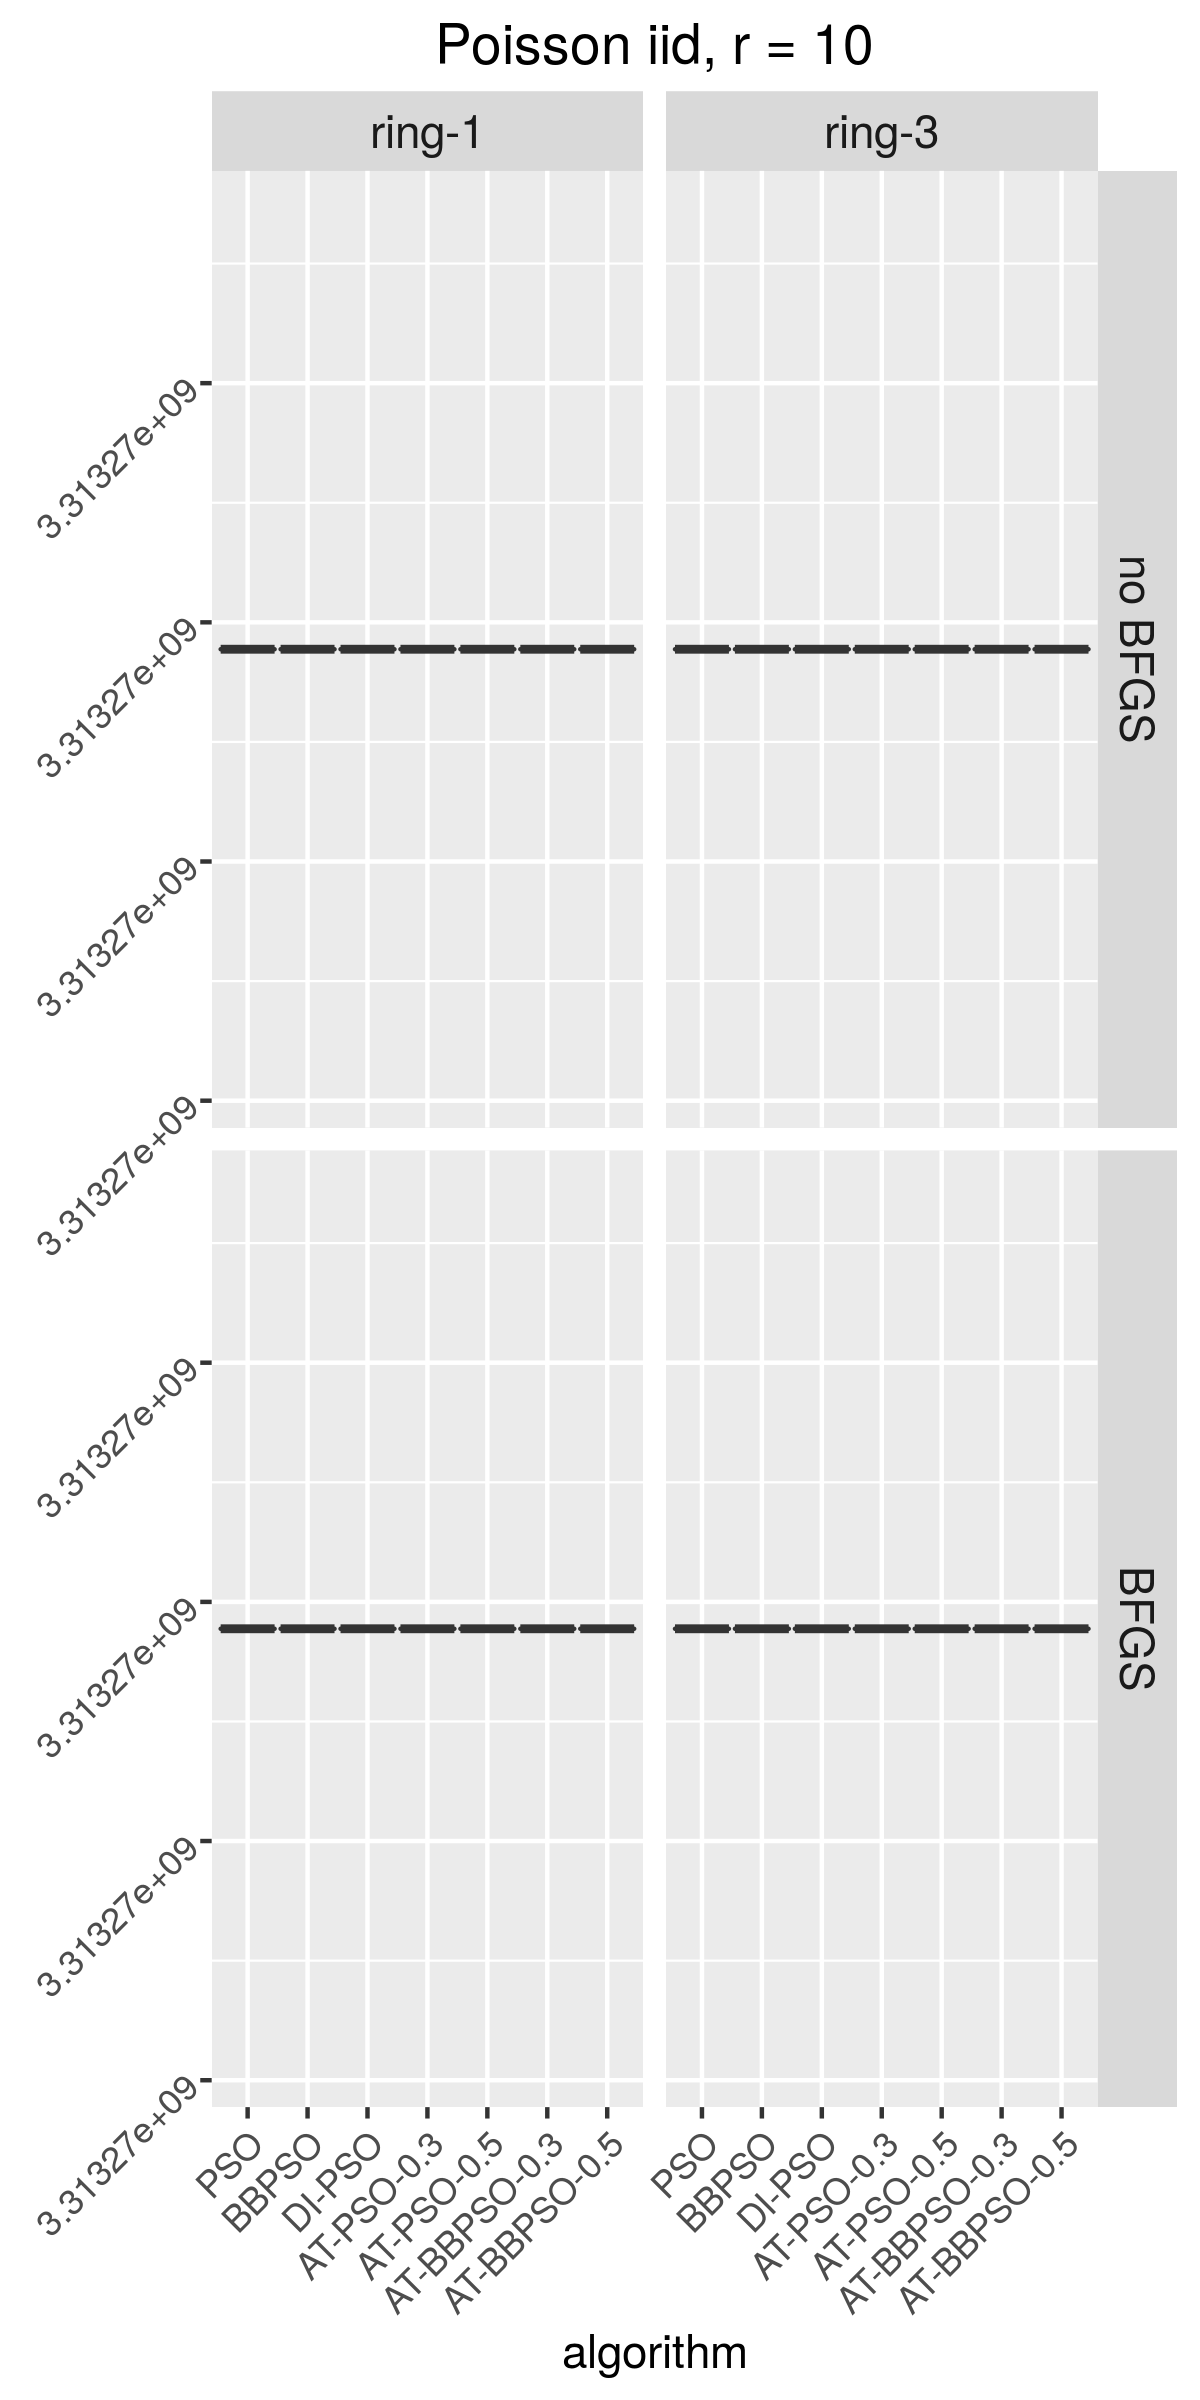
\includegraphics[width=0.4\textwidth]{pop/maxplot11.png}
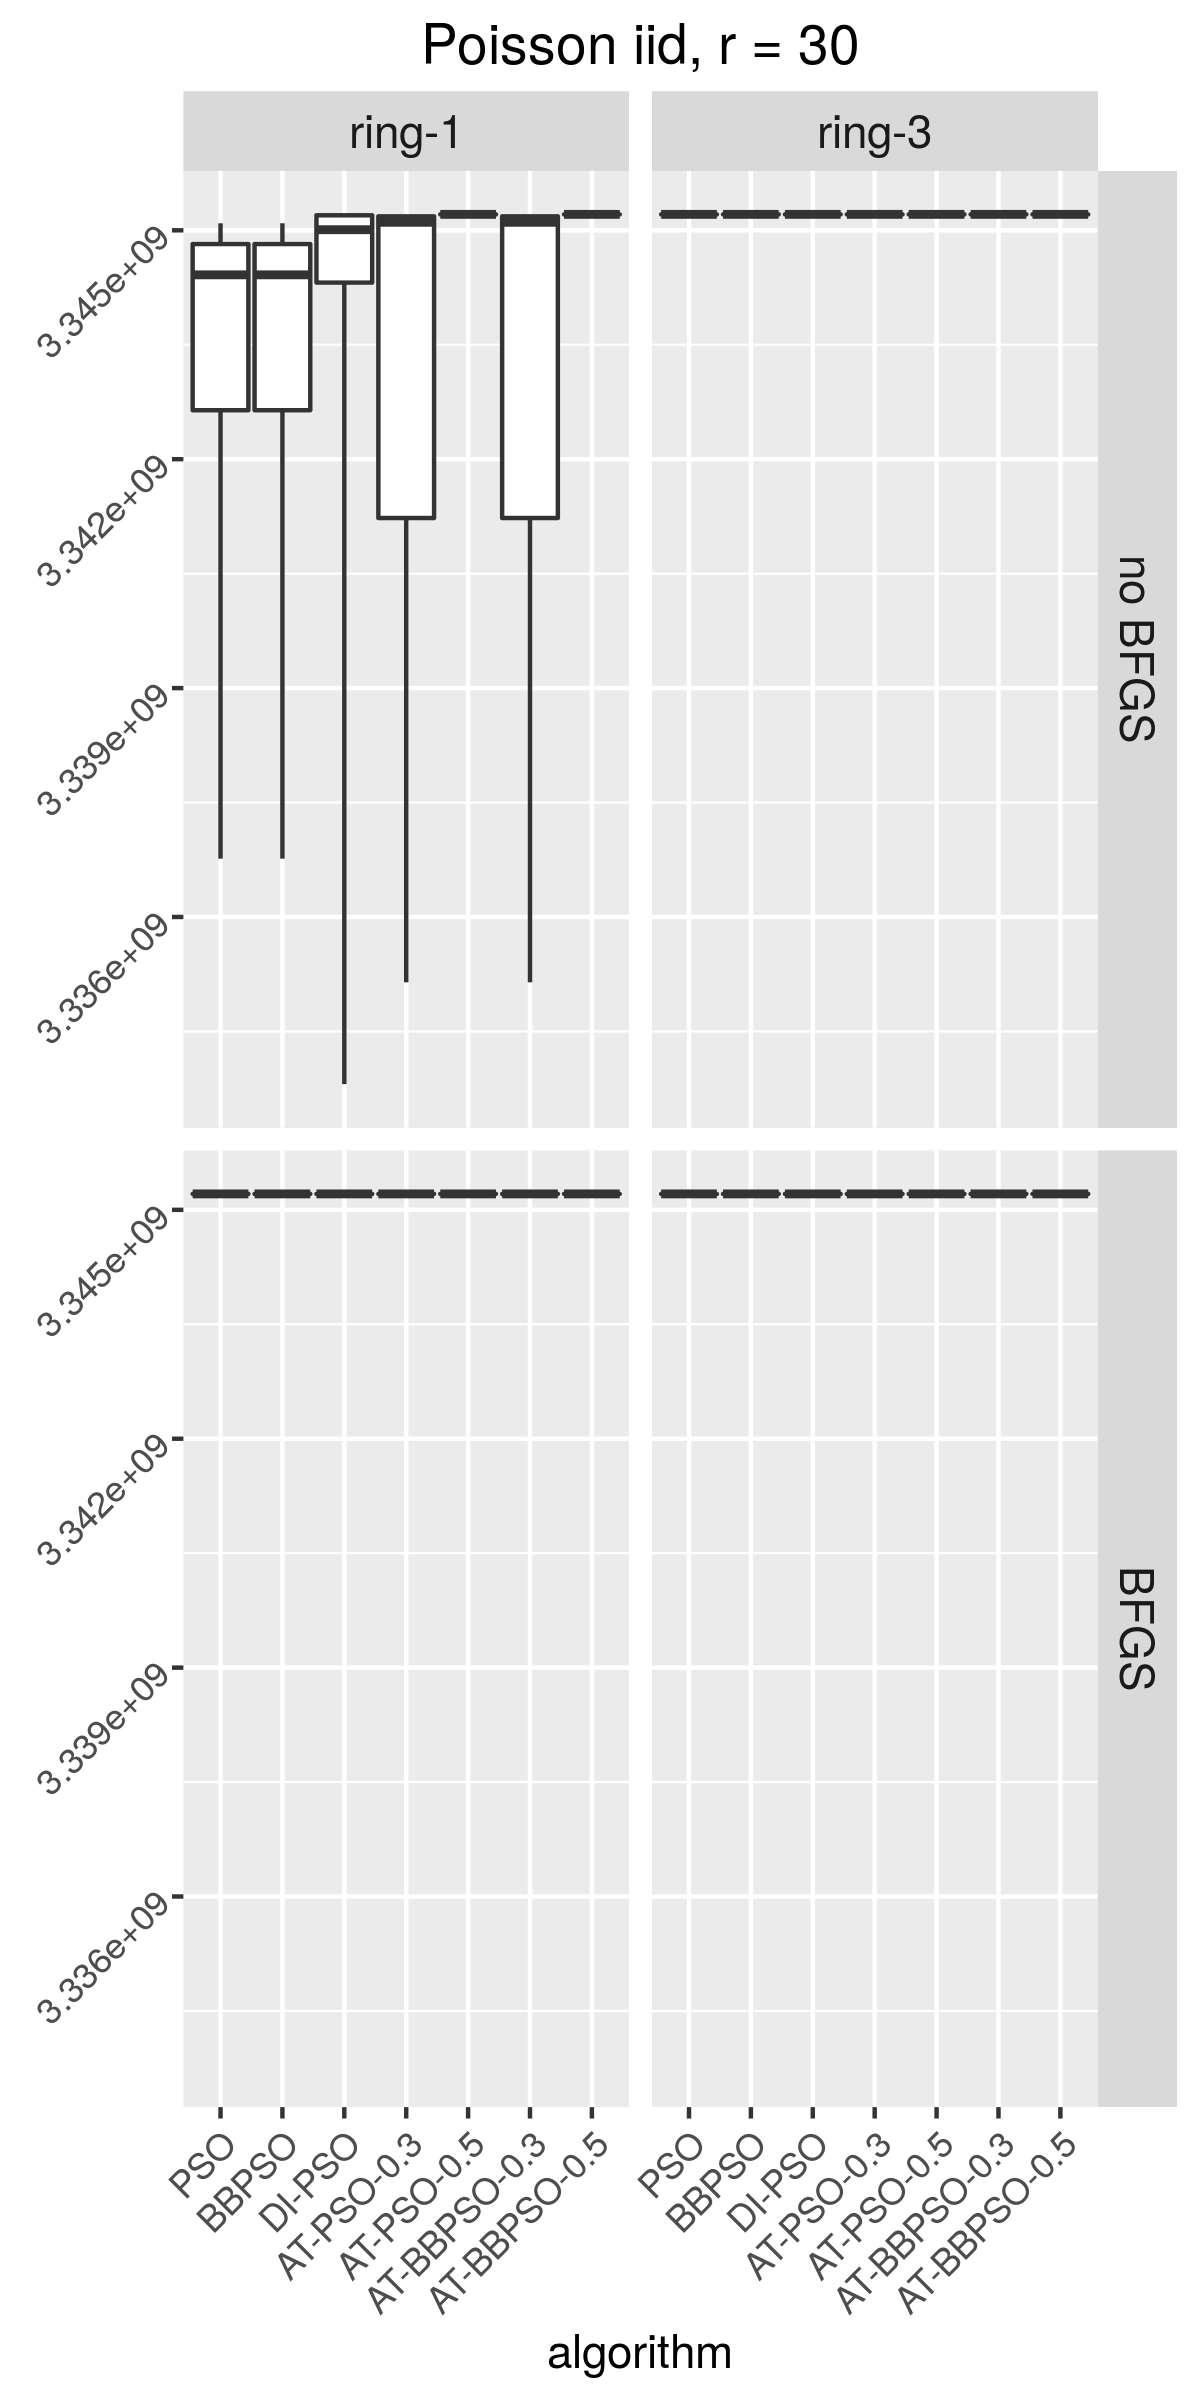
\includegraphics[width=0.4\textwidth]{pop/maxplot12.png}
%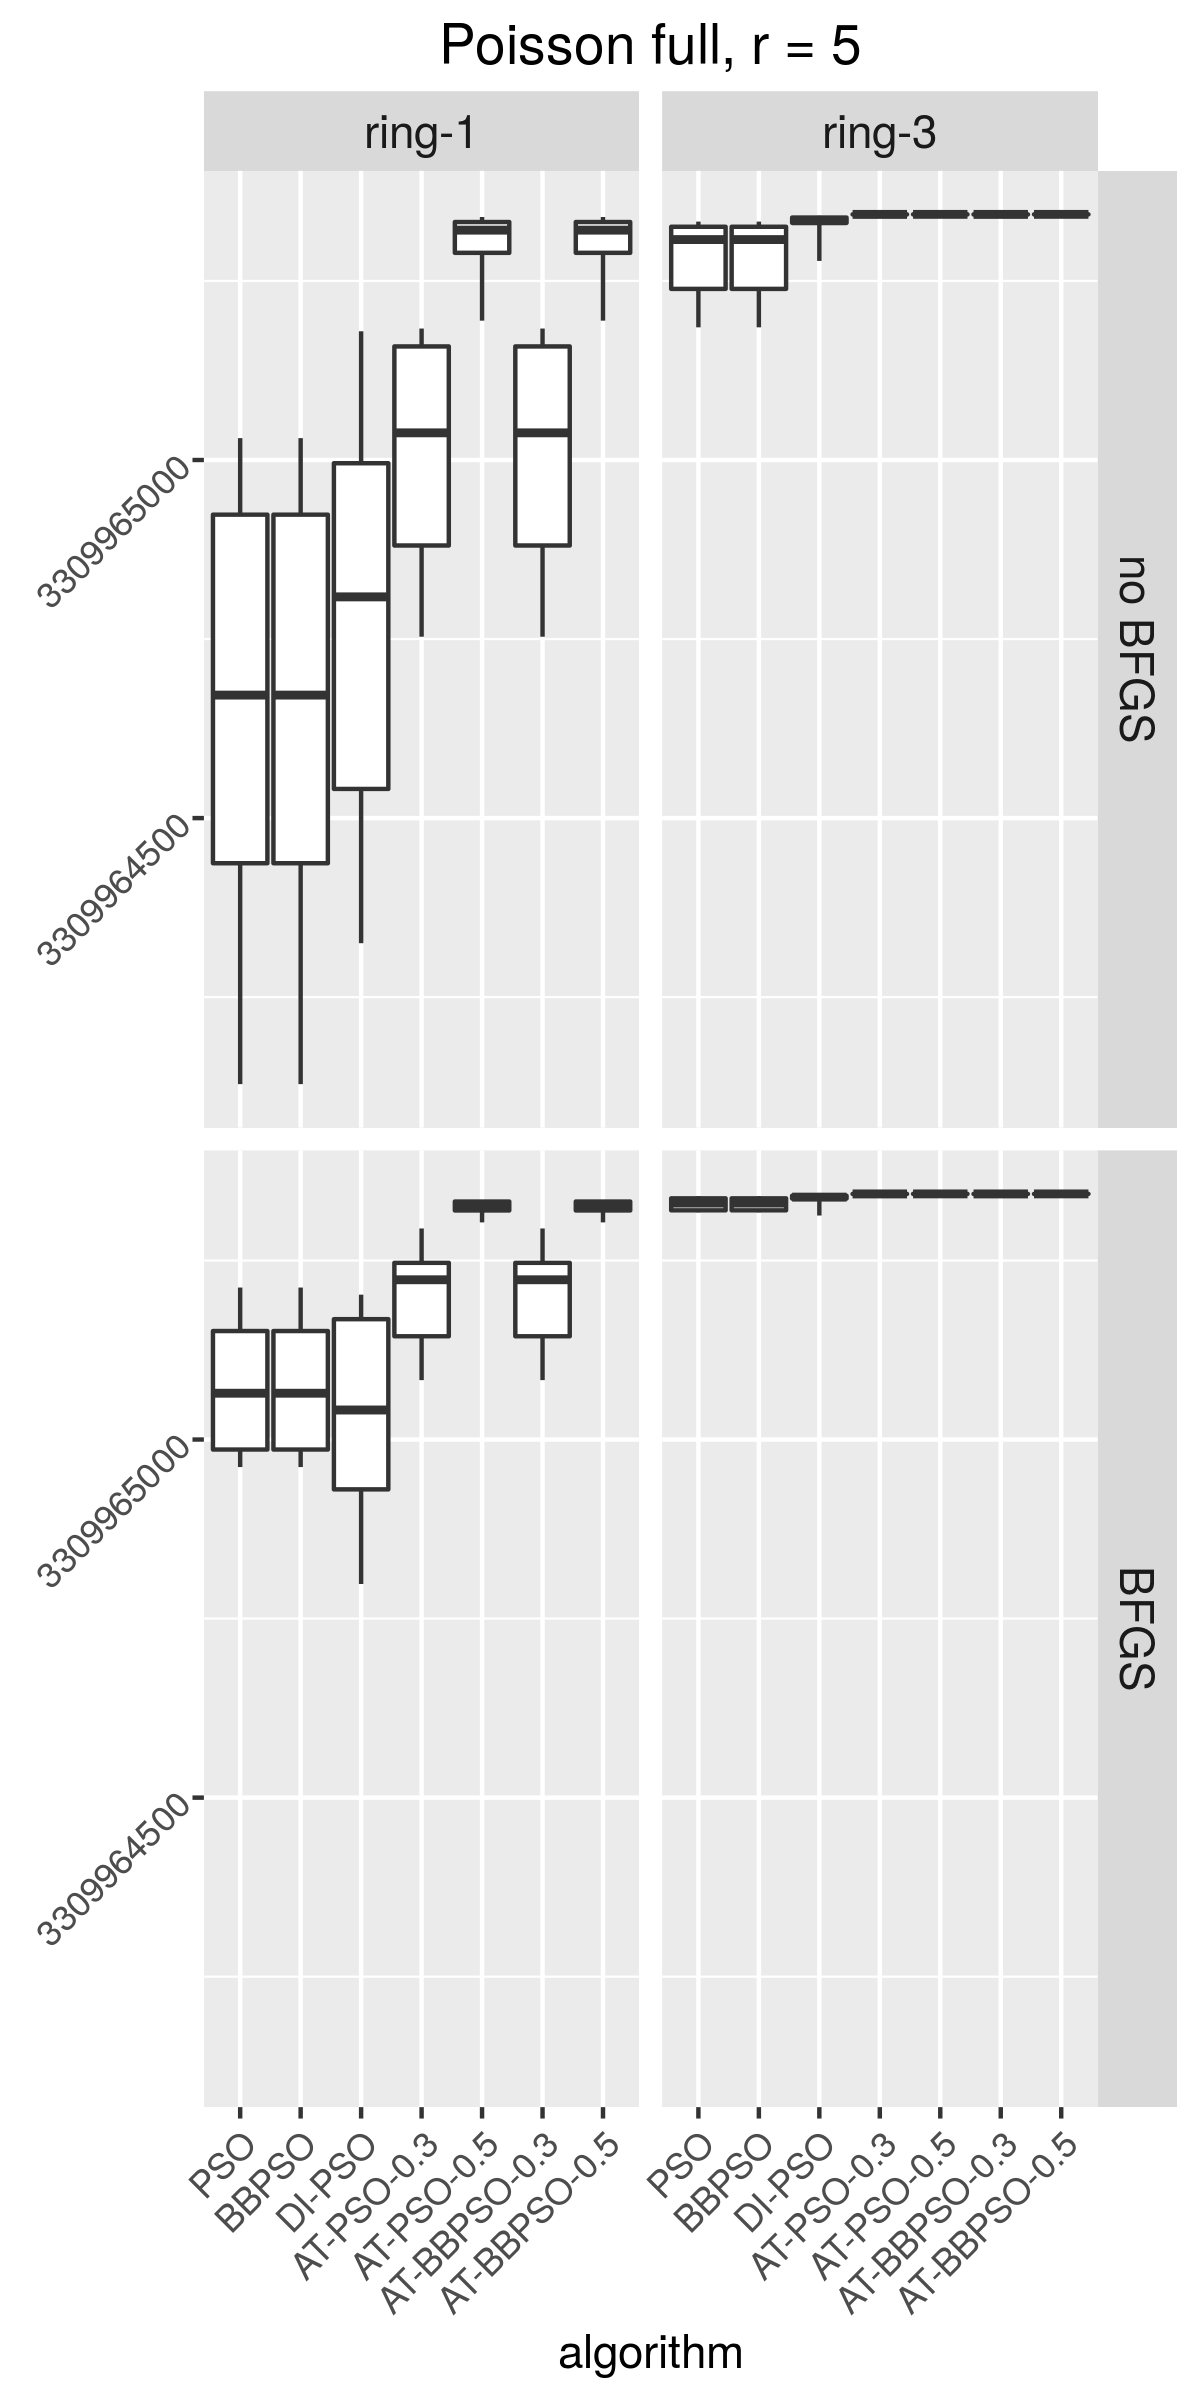
\includegraphics[width=0.4\textwidth]{pop/maxplot13.png}
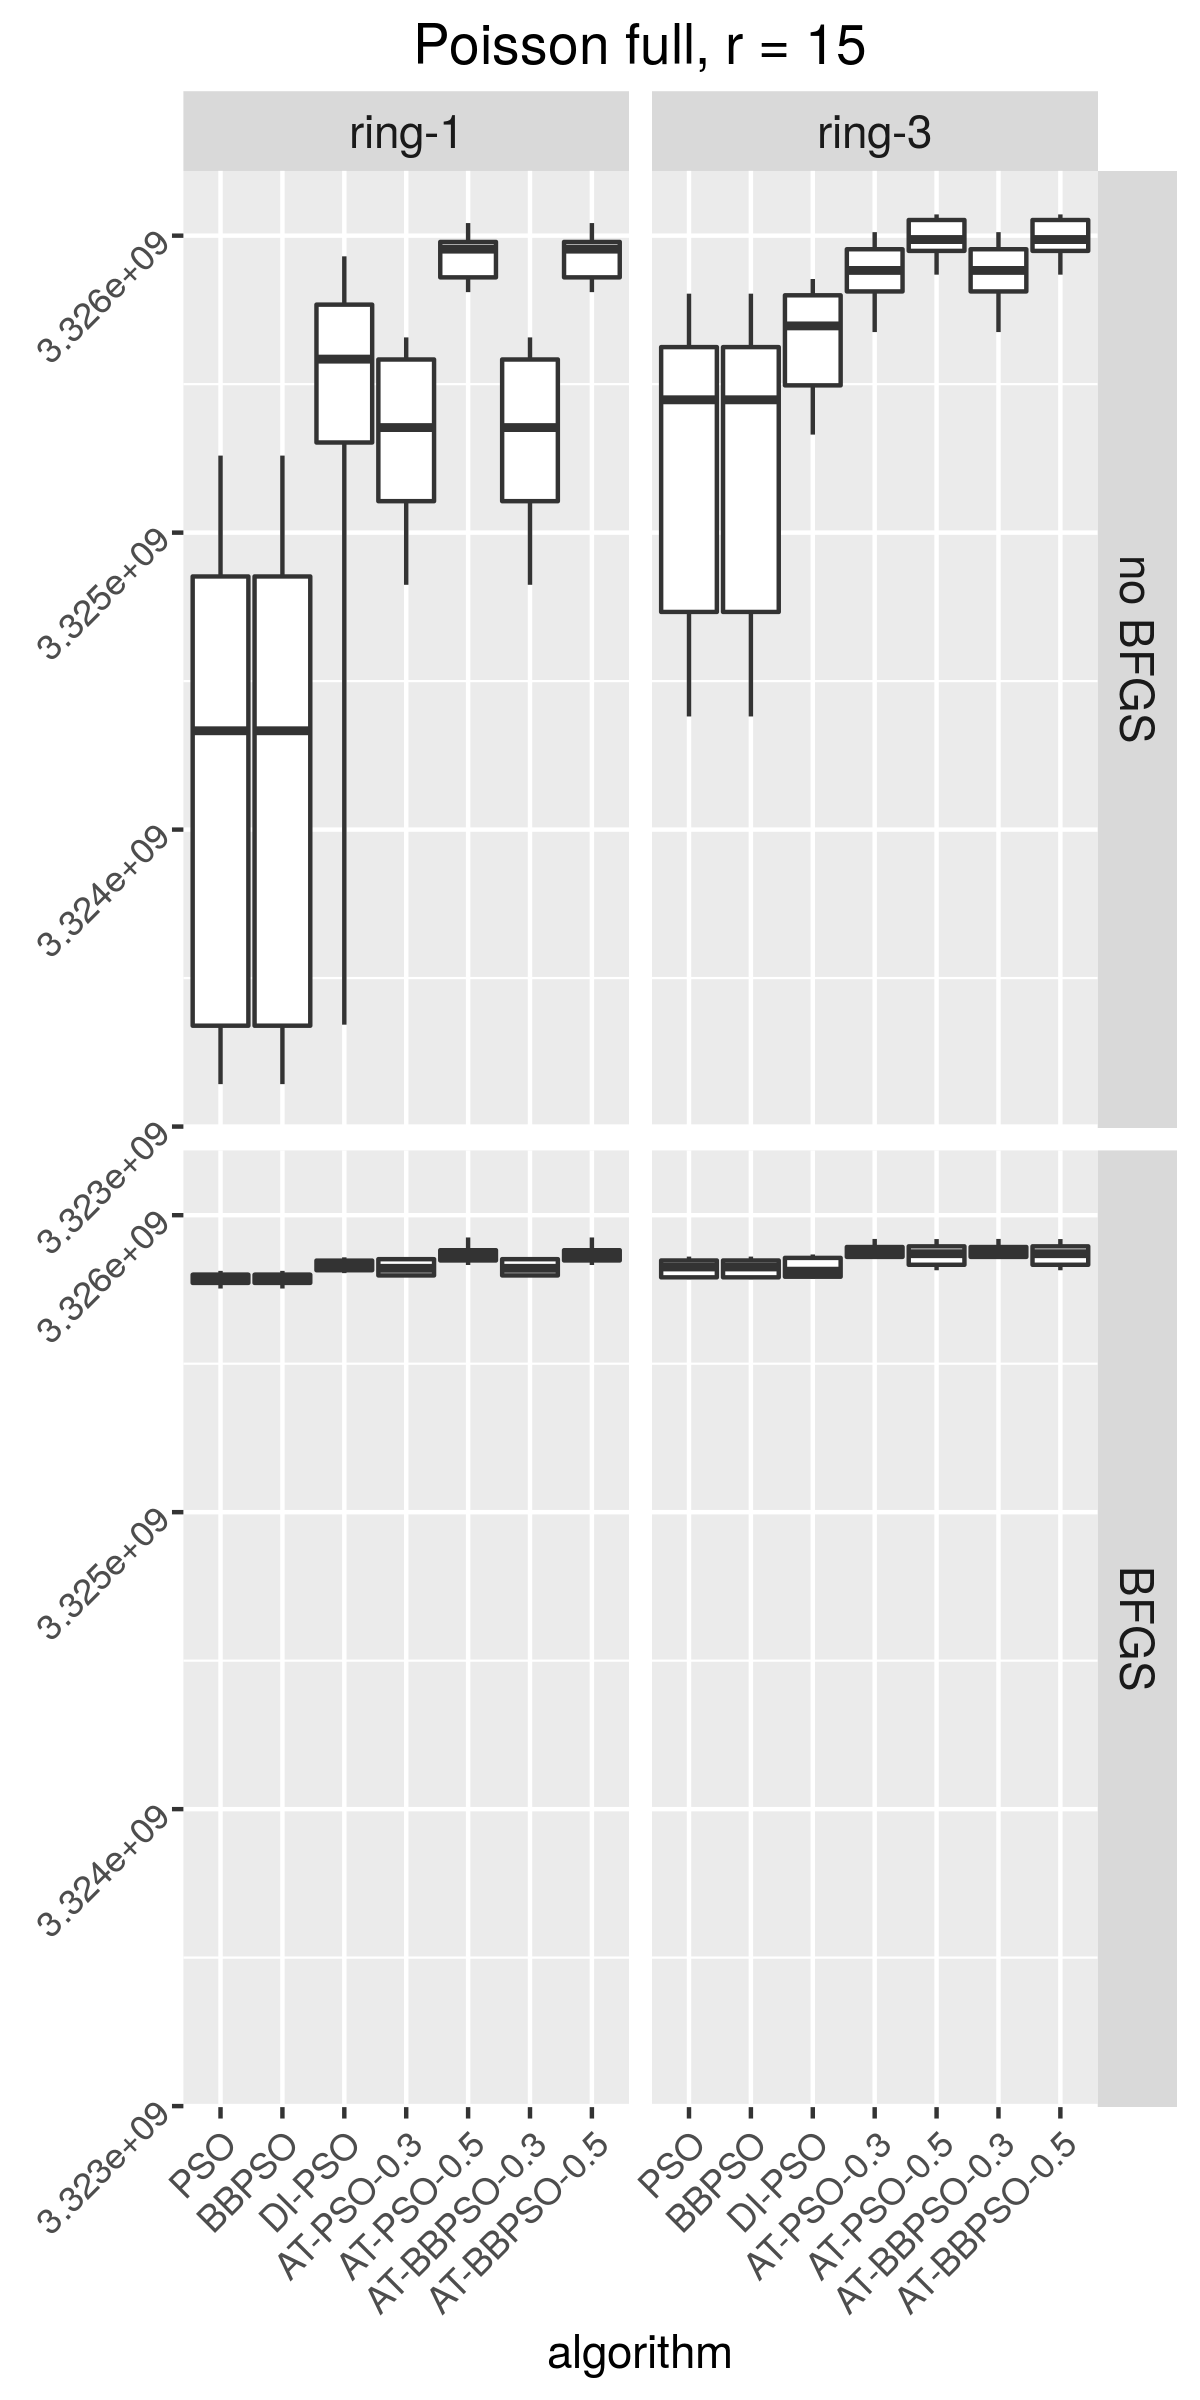
\includegraphics[width=0.4\textwidth]{pop/maxplot14.png}
\caption{Boxplots of the maximum value of the log posterior found for Poisson models by random effect type, neighborhood topology, optimization initialization, and algorithm. Each box plot was created using the 10, 25, 50, 75, and 90 percentiles of the maximum found from 20 replications of 1,000 iterations with 50 particles for each factor combination.}
\label{fig:popmaxboxplot}
\end{figure}

\begin{figure}[!ht]
\centering
%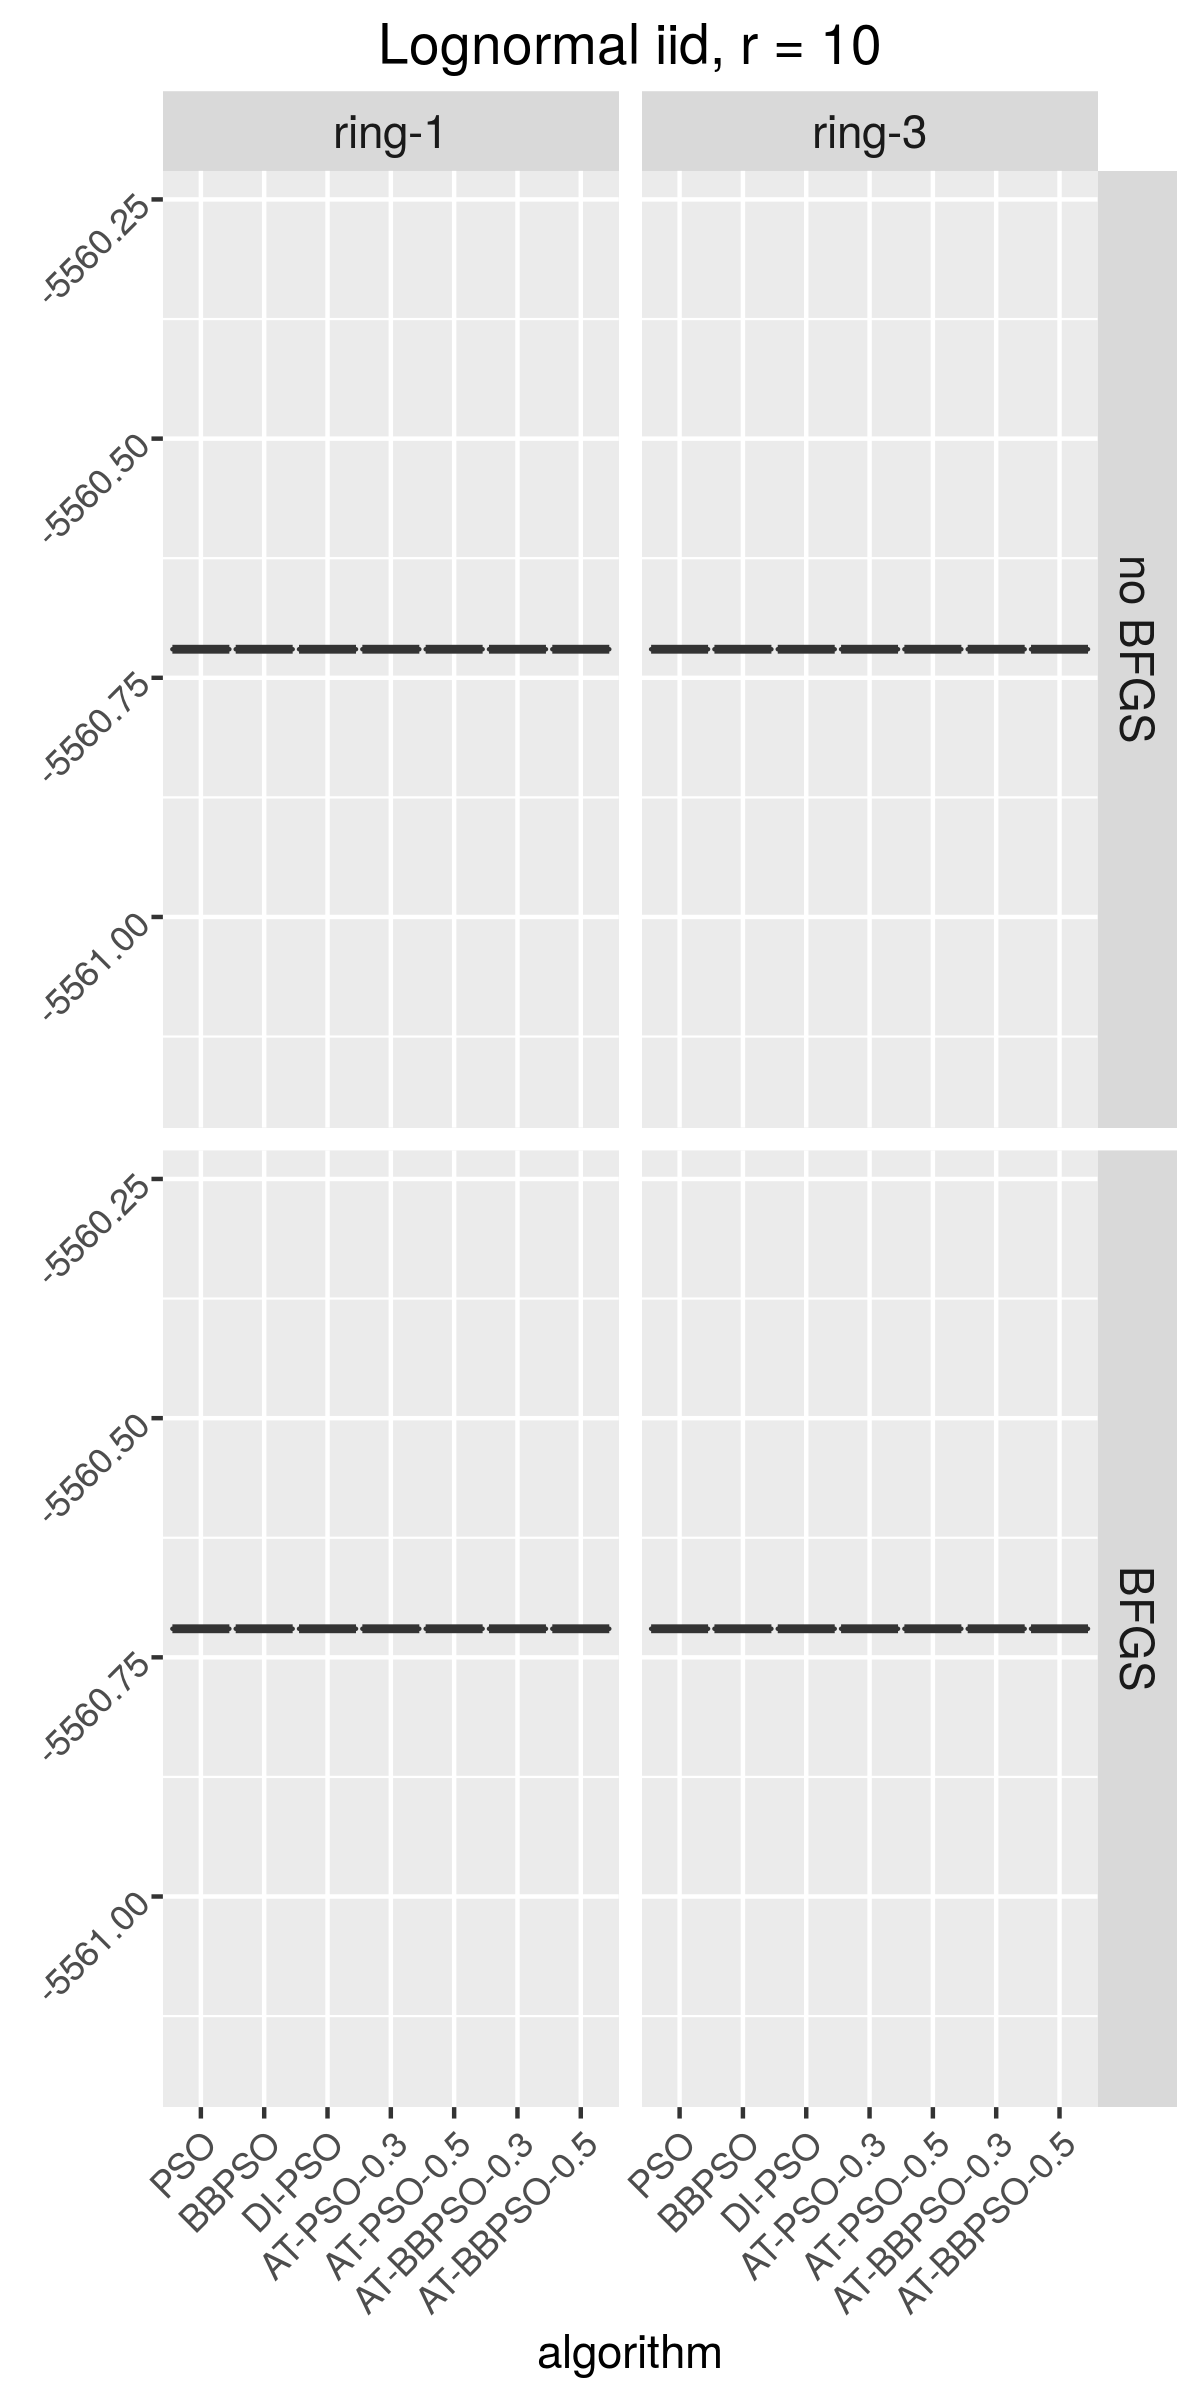
\includegraphics[width=0.4\textwidth]{pop/maxplot21.png}
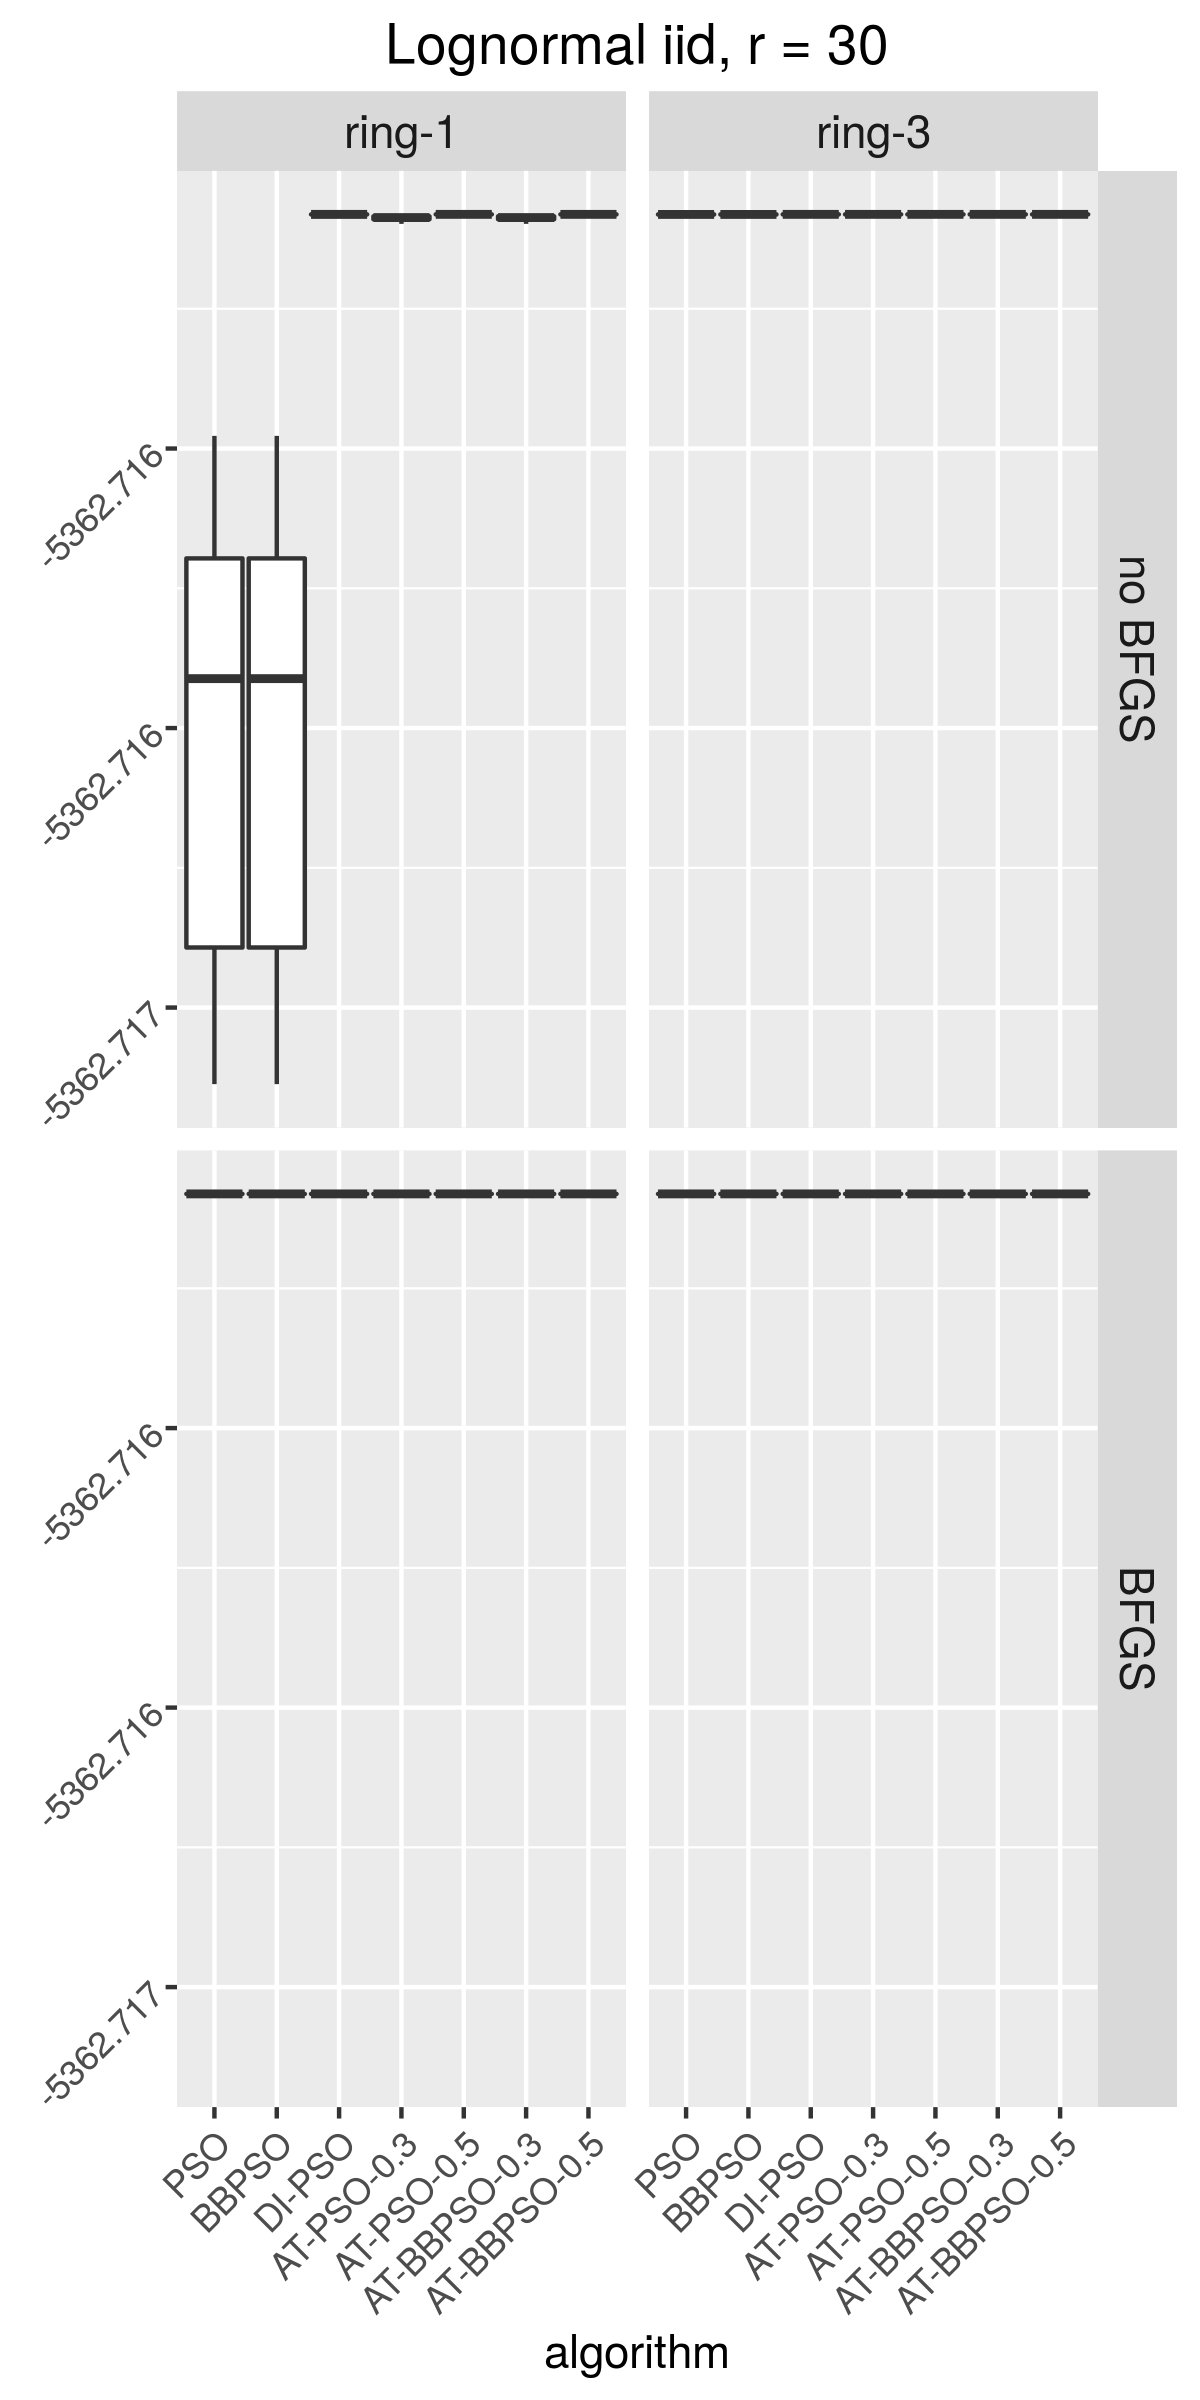
\includegraphics[width=0.4\textwidth]{pop/maxplot22.png}
%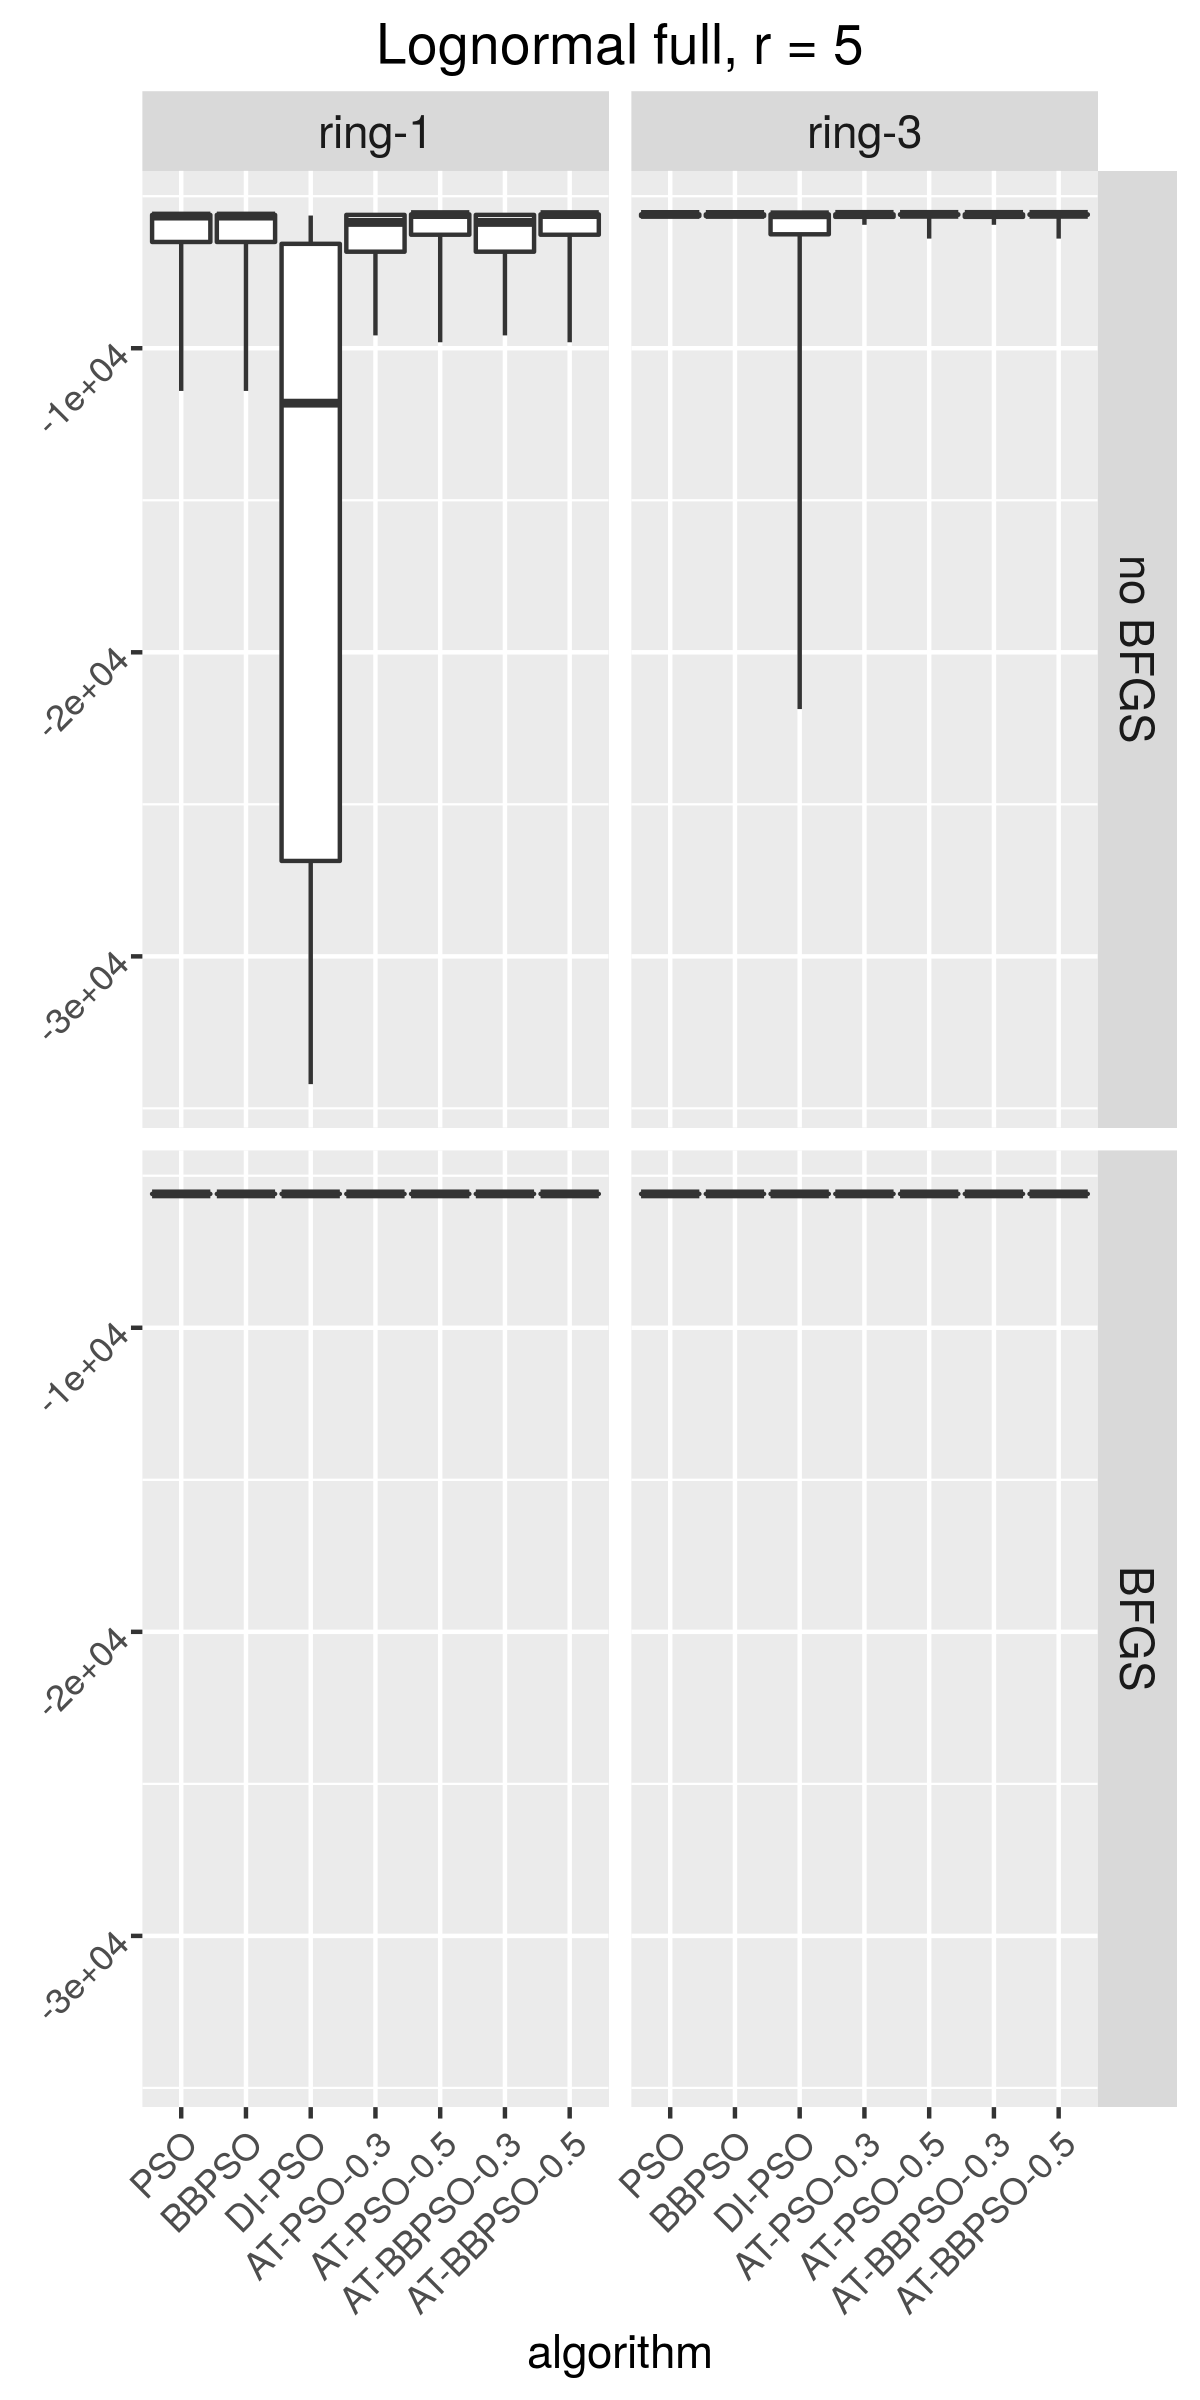
\includegraphics[width=0.4\textwidth]{pop/maxplot23.png}
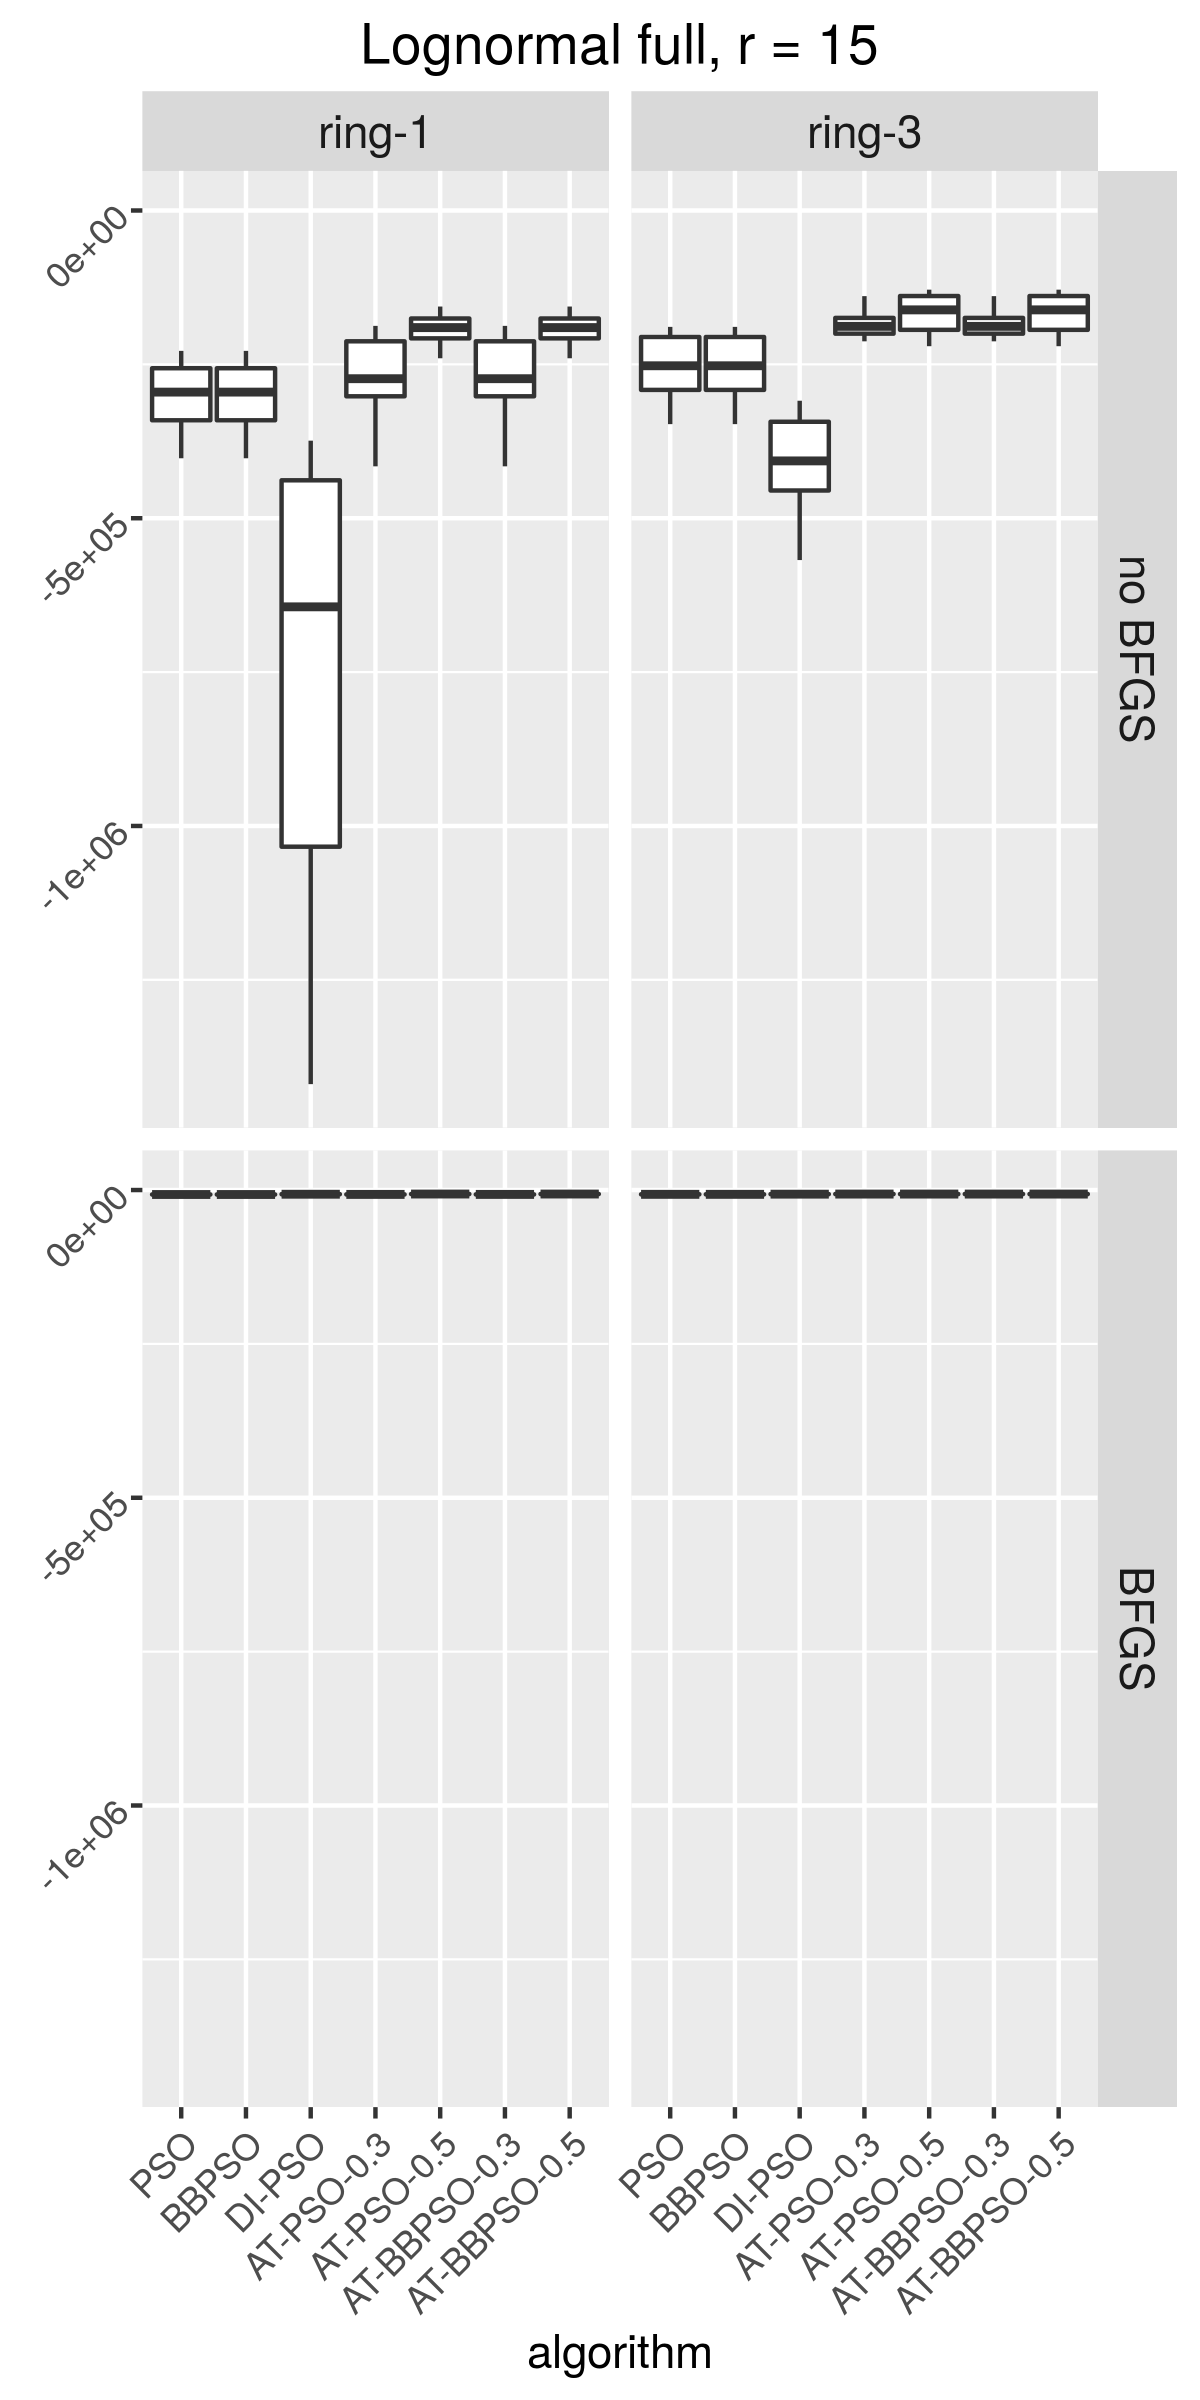
\includegraphics[width=0.4\textwidth]{pop/maxplot24.png}
\caption{Boxplots of the maximum value of the log posterior found for lognormal models by random effect type, number of random effects, neighborhood topology, optimization initialization, and algorithm. Each box plot was created using the 10, 25, 50, 75, and 90 percentiles of the maximum found from 20 replications of 1,000 iterations with 50 particles for each factor combination.}
\label{fig:popmaxboxplot2}
\end{figure}

[PARAGRAPH OR TWO AND PLOTS FOR THE ELECTION MODELS]

For our purposes, the PSO algorithms are useful only insofar as they allow us to construct IMH and IMHwG algorithms. So we conduct another simulation study to see when each algorithm gets close enough to the posterior mode for the IMH and IMHwG algorithms to have high acceptance rates. To this end we conduct another simulations study using the same 7 PSO algorithms from the previous study, except only using the ring-3 neighborhood topology and BFGS initialization. Next, we run Algorithms \ref{alg:IM1} and \ref{alg:IM2} after 0, 100, 500, 1,000, 1,500, and 2,000 iterations of the PSO algorithm and compute the acceptance rate after 1,000 iterations of the MCMC algorithm. Each MCMC algorithm is initialized at the PSO estimate of the posterior mode used to construct the Laplace approximation. When we run the IMH and IMHwG algorithms after 0 iterations of a PSO algorithm we still run the BFGS initialization, so this serves as a control to see if running the PSO algorithm is necessary to get reasonable acceptance rates. Additionally, we run each IMH and IMHwG algorithm with different choices for the degrees of freedom parameter in the Laplace approximation.

Algorithm~\ref{alg:IM1} applies straightforwardly to each of our models, though see Appendix \ref{sec:hess} for a detailed derivation of the Hessian for the county population models with a fully parameterized covariance matrix associated, i.e. from equations \eqref{eq:fullnormpostchol} and \eqref{eq:fullpoispostchol}. To apply Algorithm~\ref{alg:IM2} in the county population models, we draw $(\bm{\beta},\bm{\delta})$ in the Metropolis step and either $\sigma^2$ or $\bm{L}$ in the conditionally conjugate step, depending on the model. The full conditional distribution of $\sigma^2$ in \eqref{eq:iidnormpost} and \eqref{eq:iidpoispost} is $IG(a_{\sigma} + r/2, b_{\sigma} + \bm{\delta}'\bm{\delta}/2)$. The full conditional distribution of $\bm{\Omega}$ in \eqref{eq:fullnormpostprec} and \eqref{eq:fullpoispostprec} is $W(r + 1, (\bm{E} + \bm{\delta}\bm{\delta}')^{-1})$. Then a draw from the full conditional distribution of $\bm{L}$ can be obtained via the Bartlett decomposition as described at the end of Section~\ref{sec:pop}. In the lognormal models the full conditional distribution of $\phi^2$ is $IG(a_{\phi} + n/2, b_{\phi} + (\log \bm{z} - \bm{X}\bm{\beta} - \bm{S}\bm{\delta})'(\log \bm{z} - \bm{X}\bm{\beta} - \bm{S}\bm{\delta})/2)$. 

In single poll model of Section~\ref{sec:pres}, we draw $(\beta_0, \beta_f, \beta_b, \bm{\alpha}_{s}, \bm{\alpha}_{ae})$ in the Metropolis step, while in the all polls model we draw all of those parameters and additionally $\bm{\alpha}_p$ in the Metropolis step. Then for both models there are two additional Gibbs steps --- one where each random effect variance is drawn, and one where $(\beta_{prev}, \bm{\alpha}_r)$ is drawn. These full conditionals are straightforward to derive, so we do not reproduce them here. Likewise, the Hessian is easy though tedious to derive, so we omit it as well.

[SIMULATION STUDY TO BE COMPLETED AND PUT HERE - WON'T TAKE VERY LONG, ~ 1 DAY]

% In their conditional posterior, the random effects variances are independent with
% \begin{align*}
% \sigma^2_{s} &\sim IG\left(a_{s} + 51/2, b_{s} + \sum_{k=1}^{51}(\alpha_{s}[k] - \alpha_r[r_k] - prev_k\beta_{prev})^2/2\right)\\
% \sigma^2_{ae} &\sim IG(a_{ae} + 16/2, b_{ae} + \bm{\alpha}_{ae}'\bm{\alpha}_{ae}/2)\\
% \sigma^2_{p} &\sim IG(a_{p} + 7/2, b_{p} + \bm{\alpha}_{p}'\bm{\alpha}_{p}/2)\\
% \sigma^2_{r} &\sim IG(a_{r} + 5/2, b_{r} + \bm{\alpha}_{r}'\bm{\alpha}_{r}/2)
% \end{align*}
% where in the prior we set $a_{s}=a_{ae}=a_p=a_r=b_{s}=b_{ae}=b_p=b_r=1$. These full conditionals apply to both the single poll and all polls models, except $\sigma_p^2$ is not included

% First we consider the acceptance rates of the PSO assisted IMH and IMHwG algorithms. Table \ref{tab:accrates} contains computed acceptance rates for each of the PSO assisted algorithms and for each model for spatially smoothing county population estimates. For each model we used the default PSO algorithm to find the posterior mode with a swarm of 50 particles run for 1000 iterations using the ring-1 neighborhood. For any given model and choice of $df$ the IMH within Gibbs algorithm tends to have a higher acceptance rate --- indeed for the full Poisson model with $r=5$ or $r=7$, only the IMH winin Gibbs algorithms yields acceptable acceptance rates. The $t$ proposal also tends to do better with higher $df$ indicating that tails of the posterior are approximately normal --- indeed a $t$ distribution with $df=100$ is nearly identical to a normal distribution. Also notable is that acceptance rates for the lognormal model tend to be higher than for the Poisson model, illustrating that the closer the data model is to Gaussian the better the IMH and IMHwG algorithms based on the Laplace approximation are going to perform.

% \begin{table}[ht]
% \captionsetup{font=footnotesize}
% \centering
% \subfloat[PSO assisted independent Metropolis Hastings acceptance rates]{
% \footnotesize{
% \begin{tabular}{r|rrr|rrr|rrr|rrr}
% \multicolumn{1}{c}{IMH\phantom{wG}} & \multicolumn{3}{c}{iid lognormal}&\multicolumn{3}{c}{iid Poisson} & \multicolumn{3}{c}{full lognormal}&\multicolumn{3}{c}{full Poisson}\\
%   \hline
% df & r = 10 & 20 & 30 & 10 & 20 & 30 & 5 & 7 & 9 & 5 & 7 & 9 \\  
%   \hline
% 1 & 0.24 & 0.19 & 0.15 & 0.29 & 0.23 & 0.09 & 0.00 & 0.00 & 0.00 & 0.01 & 0.00 & 0.01 \\ 
%   4 & 0.47 & 0.37 & 0.32 & 0.54 & 0.45 & 0.18 & 0.01 & 0.00 & 0.00 & 0.01 & 0.00 & 0.00 \\ 
%   10 & 0.60 & 0.52 & 0.46 & 0.71 & 0.63 & 0.25 & 0.02 & 0.00 & 0.00 & 0.03 & 0.00 & 0.00 \\ 
%   100 & 0.72 & 0.70 & 0.68 & 0.88 & 0.88 & 0.37 & 0.02 & 0.00 & 0.00 & 0.03 & 0.01 & 0.00 \\ 
%    \hline
% \end{tabular}}}\\
% %\vspace*{0.5 cm}
% \subfloat[PSO assisted independent Metropolis Hastings within Gibbs acceptance rates]{
% \footnotesize{
% \begin{tabular}{r|rrr|rrr|rrr|rrr}
% \multicolumn{1}{c}{IMHwG} & \multicolumn{3}{c}{iid lognormal}&\multicolumn{3}{c}{iid Poisson} & \multicolumn{3}{c}{full lognormal}&\multicolumn{3}{c}{full Poisson}\\
%   \hline
% df & r = 10 & 20 & 30 & 10 & 20 & 30 & 5 & 7 & 9 & 5 & 7 & 9 \\  
%   \hline
% 1 & 0.31 & 0.23 & 0.19 & 0.31 & 0.23 & 0.11 & 0.01 & 0.00 & 0.00 & 0.17 & 0.17 & 0.06 \\ 
%   4 & 0.58 & 0.46 & 0.40 & 0.58 & 0.46 & 0.18 & 0.01 & 0.00 & 0.00 & 0.57 & 0.12 & 0.07 \\ 
%   10 & 0.75 & 0.65 & 0.56 & 0.76 & 0.64 & 0.27 & 0.01 & 0.00 & 0.00 & 0.44 & 0.11 & 0.09 \\ 
%   100 & 0.94 & 0.92 & 0.89 & 0.96 & 0.94 & 0.36 & 0.02 & 0.00 & 0.00 & 0.50 & 0.14 & 0.03 \\ 
%    \hline
% \end{tabular}}}
% \caption{ Acceptance rates for the PSO assisted IMH algorithm (a) and the IMH within Gibbs algorithm (b) in the Poisson and lognormal models with either iid or fully correlated random effects. For each algorithm and each model the initial posterior mode was estimated using the default PSO algorithm, then acceptance rates were computed from a sample of 9000 after a burn-in of 1000. The parameter $r$ denotes the number of random effects in the model and $df$ denotes the degrees of freedom parameter used in the $t$ proposal.}
% \label{tab:accrates}
% \end{table}

% Both the full Poisson and full lognormal model cause problems because the fully parameterized covariance matrix means that the normal approximation will be poor for those parameters. In the iid case the random effect variance essentially has $r$ observations --- one for each random effect --- but in the full model we have an $r\times r$ covariance matrix with essentially one observation ($\bm{\delta}$). The Laplace approximation is an asymptotic result so with such a small amount of data it is no surprise that it is poor. However, IMHwG still works well for the Poisson model when the dimension of $\bm{\delta}$ is small enough --- in this case $r=5$. The conditional posterior of $(\bm{\beta}, \bm{\delta})$ given $\bm{L}$ should approximated well by a $t$ distribution even for larger $r$ given the amount of observed data and the normal priors on $\bm{\beta}$ and $\bm{\delta}$. The problem is that our estimate of the mode is poor, though this can be solved with enough patience.

% While Table \ref{tab:accrates} used the same PSO algorithm to investigate acceptance rates, Table \ref{tab:longaccrates} uses a variety of different PSO algorithms. Four algorithms are considered: standard PSO, BBPSOxp-MC, AT-BBPSOxp-MC with $df=1$ and $R^*=0.1$, and AT-BBPSOxp-MC with $df=5$ and $R^*=0.3$. Each algorith was run with 1,000 particles in a ring-1 neighborhood for 10,000 iterations. Finally, the IMH and IMHwG MCMC algorithms were run multiple times for each PSO algorithm, using the PSO algorithm's estimate of the mode after 100, 1,000, 5,000, and 10,000 iterations. A key takeaway from Table \ref{tab:longaccrates} is that in many conditions the main reason that IMH and IMHwG have poor acceptance rates is that the PSO algorithm has failed to adequately estimate the posterior mode. In Table \ref{tab:accrates}, both algorithms had trouble with the fully parameterized Poisson model. But using a larger swarm size and many more iterations, the standard PSO algorithm yields IMH algorithms with low but acceptable acceptance rates and IMHwG algrithms with near 100\% acceptance rates --- at least for $r=5$ and $r=10$. For $r=15$ the MCMC algorithm fails, but examination of Figure \ref{fig:longpsopoisfull15} shows that the PSO algorithm has not converged even after 10,000 iterations. Running the algorithm longer or using the same amount of iterations with a larger swarm size could result in convergence and, as a result, yield better Metropolis acceptance rates at the cost of more time spent on computation. The upshot is that at least for the Poisson model using this data, the IMHwG algorithm seems to always have near 100\% acceptance rates if you can find the posterior mode. As the dimension of the optimization problem grows, however, this becomes an increasingly costly problem to solve.

% \begin{table}[ht]
% \captionsetup{font=footnotesize}
% \centering
% \subfloat[PSO assisted independent Metropolis Hastings acceptance rates]{
% \footnotesize{
% \begin{tabular}{l|r|rrr|rrr|rrr|rrr}
% \multicolumn{2}{l}{IMH} & \multicolumn{3}{c}{iid lognormal} & \multicolumn{3}{c}{iid Poisson} & \multicolumn{3}{c}{full lognormal} & \multicolumn{3}{c}{full Poisson} \\
%   \hline
% \multicolumn{1}{c|}{PSO alg} & \multicolumn{1}{c|}{$n_{\text{iter}}$} & r = 10 & 30 & 50 & 10 & 30 & 50 & 5 & 10 & 15 & 5 & 10 & 15\\
%   \hline
% PSO & 100 & 0.21 & 0.02 & 0.01 & 0.00 & 0.43 & 0.50 & 0.01 & 0.00 & 0.00 & 0.04 & 0.10 & 0.18 \\ 
% BBPSOxp-MC&  & 0.59 & 0.02 & 0.00 & 0.31 & 0.12 & 0.24 & 0.01 & 0.00 & 0.00 & 0.02 & 0.03 & 0.04 \\ 
% AT-1-0.1 &  & 0.67 & 0.00 & 0.00 & 0.23 & 0.00 & 0.30 & 0.00 & 0.00 & 0.00 & 0.01 & 0.03 & 0.05 \\ 
% AT-5-0.3 &  & 0.55 & 0.01 & 0.00 & 0.31 & 0.12 & 0.27 & 0.01 & 0.00 & 0.00 & 0.03 & 0.03 & 0.06 \\ 
% \hline
% PSO & 1,000 & 0.71 & 0.67 & 0.58 & 0.89 & 0.25 & 0.01 & 0.01 & 0.00 & 0.00 & 0.27 & 0.01 & 0.04 \\ 
% BBPSOxp-MC&  & 0.71 & 0.66 & 0.51 & 0.88 & 0.01 & 0.02 & 0.01 & 0.00 & 0.00 & 0.02 & 0.00 & 0.01 \\ 
% AT-1-0.1 &  & 0.72 & 0.66 & 0.53 & 0.88 & 0.01 & 0.02 & 0.01 & 0.00 & 0.00 & 0.04 & 0.01 & 0.01 \\ 
% AT-5-0.3 &  & 0.71 & 0.65 & 0.54 & 0.88 & 0.02 & 0.02 & 0.01 & 0.00 & 0.00 & 0.05 & 0.00 & 0.01 \\ 
% \hline
% PSO & 5,000 & 0.70 & 0.66 & 0.54 & 0.89 & 0.88 & 0.85 & 0.03 & 0.00 & 0.00 & 0.00 & 0.05 & 0.02 \\ 
% BBPSOxp-MC&  & 0.73 & 0.64 & 0.54 & 0.89 & 0.01 & 0.01 & 0.00 & 0.00 & 0.00 & 0.20 & 0.00 & 0.01 \\ 
% AT-1-0.1 &  & 0.72 & 0.68 & 0.58 & 0.89 & 0.10 & 0.00 & 0.04 & 0.00 & 0.00 & 0.37 & 0.00 & 0.01 \\ 
% AT-5-0.3 &  & 0.71 & 0.67 & 0.55 & 0.89 & 0.01 & 0.01 & 0.01 & 0.00 & 0.00 & 0.13 & 0.00 & 0.01 \\ 
% \hline
% PSO & 10,000 & 0.69 & 0.66 & 0.55 & 0.89 & 0.88 & 0.84 & 0.03 & 0.00 & 0.00 & 0.35 & 0.42 & 0.01 \\ 
% BBPSOxp-MC&  & 0.71 & 0.67 & 0.54 & 0.89 & 0.00 & 0.01 & 0.02 & 0.00 & 0.00 & 0.23 & 0.00 & 0.01 \\ 
% AT-1-0.1 &  & 0.72 & 0.67 & 0.55 & 0.88 & 0.46 & 0.01 & 0.01 & 0.00 & 0.00 & 0.46 & 0.00 & 0.01 \\ 
% AT-5-0.3 &  & 0.73 & 0.67 & 0.50 & 0.88 & 0.01 & 0.01 & 0.02 & 0.00 & 0.00 & 0.50 & 0.00 & 0.01 \\ 
%    \hline
% \end{tabular}}}\\

% \subfloat[PSO assisted independent Metropolis Hastings within Gibbs acceptance rates]{
% \footnotesize{
% \begin{tabular}{l|r|rrr|rrr|rrr|rrr}
% \multicolumn{2}{l}{IMHwG} & \multicolumn{3}{c}{iid lognormal} & \multicolumn{3}{c}{iid Poisson} & \multicolumn{3}{c}{full lognormal} & \multicolumn{3}{c}{full Poisson} \\
%   \hline
% \multicolumn{1}{c|}{PSO alg} & \multicolumn{1}{c|}{$n_{\text{iter}}$} & r = 10 & 30 & 50 & 10 & 30 & 50 & 5 & 10 & 15 & 5 & 10 & 15\\
%   \hline
% PSO & 100 & 0.00 & 0.00 & 0.00 & 0.00 & 0.00 & 0.00 & 0.00 & 0.00 & 0.00 & 0.33 & 0.15 & 0.15 \\ 
% BBPSOxp-MC&  & 0.73 & 0.02 & 0.00 & 0.00 & 0.00 & 0.00 & 0.00 & 0.00 & 0.00 & 0.24 & 0.15 & 0.08 \\ 
% AT-1-0.1 &  & 0.78 & 0.02 & 0.00 & 0.00 & 0.00 & 0.00 & 0.00 & 0.00 & 0.00 & 0.29 & 0.28 & 0.08 \\ 
% AT-5-0.3 &  & 0.66 & 0.01 & 0.00 & 0.00 & 0.00 & 0.00 & 0.00 & 0.00 & 0.00 & 0.40 & 0.09 & 0.07 \\ 
% \hline
% PSO & 1,000 & 0.93 & 0.89 & 0.84 & 0.96 & 0.30 & 0.00 & 0.02 & 0.00 & 0.00 & 0.77 & 0.06 & 0.02 \\ 
% BBPSOxp-MC&  & 0.94 & 0.87 & 0.67 & 0.96 & 0.00 & 0.00 & 0.02 & 0.00 & 0.00 & 0.20 & 0.06 & 0.03 \\ 
% AT-1-0.1 &  & 0.93 & 0.90 & 0.80 & 0.97 & 0.00 & 0.00 & 0.02 & 0.00 & 0.00 & 0.37 & 0.11 & 0.04 \\ 
% AT-5-0.3 &  & 0.93 & 0.85 & 0.76 & 0.95 & 0.00 & 0.00 & 0.01 & 0.00 & 0.00 & 0.51 & 0.20 & 0.05 \\ 
% \hline
% PSO & 5,000 & 0.93 & 0.90 & 0.85 & 0.97 & 0.91 & 0.86 & 0.02 & 0.00 & 0.00 & 0.97 & 0.86 & 0.04 \\ 
% BBPSOxp-MC&  & 0.94 & 0.88 & 0.80 & 0.96 & 0.07 & 0.00 & 0.02 & 0.00 & 0.00 & 0.89 & 0.10 & 0.07 \\ 
% AT-1-0.1 &  & 0.93 & 0.89 & 0.84 & 0.96 & 0.07 & 0.00 & 0.00 & 0.00 & 0.00 & 0.95 & 0.17 & 0.08 \\ 
% AT-5-0.3 &  & 0.93 & 0.89 & 0.80 & 0.96 & 0.00 & 0.00 & 0.03 & 0.00 & 0.00 & 0.64 & 0.12 & 0.01 \\ 
% \hline
% PSO & 10,000 & 0.93 & 0.90 & 0.85 & 0.96 & 0.91 & 0.87 & 0.03 & 0.00 & 0.00 & 0.97 & 0.95 & 0.02 \\ 
% BBPSOxp-MC&  & 0.93 & 0.89 & 0.85 & 0.96 & 0.31 & 0.00 & 0.01 & 0.00 & 0.00 & 0.97 & 0.24 & 0.07 \\ 
% AT-1-0.1 &  & 0.93 & 0.90 & 0.85 & 0.96 & 0.45 & 0.00 & 0.01 & 0.00 & 0.00 & 0.97 & 0.09 & 0.06 \\ 
% AT-5-0.3 &  & 0.93 & 0.89 & 0.83 & 0.97 & 0.00 & 0.00 & 0.03 & 0.00 & 0.00 & 0.95 & 0.03 & 0.03 \\    \hline
% \end{tabular}}}
% \caption{ Acceptance rates for the PSO assisted IMH algorithm (a) and the IMH within Gibbs algorithm (b) in the Poisson and lognormal models with either iid or fully correlated random effects. For each algorithm and each model the initial posterior mode was estimated using several PSO algorithms with a swarm size of 1,000, run for $n_{\text{iter}}=$10,000 iterations. Then both the IMH and IMHwG MCMC algorithms were fit using each PSO algorithm's estimate of the mode after 100, 1,000, 5,000, and 10,000 iterations. Acceptance rates were computed by using from a sample of 9,000 after a burn-in of 1,000. The parameter $r$ denotes the number of random effects in the model. The AT-1-0.1 algorithm is AT-BBPSOxp-MC with $df=1$ and $R^*=0.1$, and similarly for AT-5-0.3.}
% \label{tab:longaccrates}
% \end{table}

% % \begin{figure}[ht]
% % \centering
% % \includegraphics[width=0.8\textwidth]{pop/poisfullplot.png}
% % \caption{Log posterior evaluation at current estimate of the posterior mode in the last 1,000 iterations of the standard PSO algorithm for the fully parameterizez Poisson model using 100 particles in the ring-1 neighborhood.}
% % \label{fig:longpsopoisfull15}
% % \end{figure}

% For the fully parameterized lognormal model, neither IMH nor IMHwG yields an acceptable acceptance rate. Even with $r=2$, a fairly easy version of the optimization problem, acceptance rates for both the IMH and the IMHwG MCMC algorithms are less than 0.25. The problem is that the normal approximation to the posterior of $(\bm{\beta}, \bm{\delta}, \bm{L})$ fails to accurately capture the dependence between $\bm{\delta}$ and $\bm{L}$, and as a result the scale matrix in the $t$ proposal is poorly adapted to the conditional covariance matrix of $\bm{\beta}, \bm{\delta}|\bm{L}$. This problem is limited to the fully parameterized lognormal model since in the iid lognormal model, acceptance rates are quite high for both the IMH and IMHwG algorithms.

% An important lesson in Tables \ref{tab:accrates} and \ref{tab:longaccrates} from both the lognormal and Poisson models is that the quality of the IMH and IMHwG algorithms based on the normal approximation to the posterior can be highly sensitive to the quality of the estimate of the posterior mode. It is worth expending some extra effort in order to ensure that the optimization algorithm has not prematurely converged or otherwise failed to find the true posterior mode --- this is true no matter which optimization algorithm we use to find the mode, whether PSO, another heuristic algorithm like a genetic algorithm, or a gradient based approach. A second feature of Table \ref{tab:longaccrates} is that it illustrates that the standard PSO algorithm works well in the statistical context we are dealing with. The Metropolis acceptance rates of the IMH and IMHwG algorithms stay high as $r$ increases when using the standard PSO estimate of the mode, but the estimates based on alternative PSO algorithms yield acceptance rates that drop off as $r$ increases. This behavior is most pronounced when using the PSO estimates after 10,000 iterations, though it is not universal. In some cases when using a low number of iterations of the PSO algorithms to estimate the posterior mode the alternative PSO algorithms yield MCMC algorithms with higher acceptance rates, but as the number of iterations used in the PSO algorithms increases the acceptance rate of the MCMC algorithms using standard PSO to estimate the mode catch up and sometimes surpass that of the MCMC algorithms based on the alternative PSO algorithms. This can be seen for the IMH algorithm in the iid Poisson and iid lognormal models with $r=10$ and for the IMHwG algorithm in the iid lognormal model with $r=10$ moving from $n_{\text{iter}}=100$ to $n_{\text{iter}}=$1,000. For the IMH algorithm in the fully parameterized Poisson model with $r=5$ moving from $n_{\text{iter}}=$1,000 to $n_{\text{iter}}=$5,000 to $n_{\text{iter}}=$10,000 it appears that something similar is occuring, though in the fully correlated models the MCMC algorithms can often get stuck for many iterations when the estimate of the posterior mode is poor.

% Essentially standard PSO allows the particles to explore the space more or less randomly at first and only after the swarm builds up information about the higher value areas of the space does the swarm begin moving in that direction. The various BBPSO variants begin moving the particles toward higher value areas more quickly at first, but are often overtaken by standard PSO when the objective function is relatively well behaved. In practice this means that standard PSO is a advantageous for estimating the posterior mode since the quality of the normal approximation as a Metropolis-Hastings proposal is highly sensity to the quality of the estimate of the posterior mode. If the log posterior is less well behaved and the normal approximation is still desired, AT-BBPSO variants may be better suited to the problem since they appear to be more robust to complicated objective functions as seen in Appendix \ref{sec:psocompare}. In other statistical estimation contexts where stronger optimization power is desired but it is not so crucial to exactly find the optimum, AT-BBPSO variants again seem advantageous.


\section{Comparison of MCMC techniques}\label{sec:compest}

Next we move to comparing various MCMC algorithms for both classes of models. The other MCMC algorithms we consider in this section are single move random walk Metropolis within Gibbs (RWwG), block random walk Metropolis within Gibbs (B-RWwG), Hamiltonian Monte Carlo as implemented by the Stan software \citep{carpenter2015stan} using the No U-turn Sampler \citep{homan2014no} and for the lognormal model for county populations, a two step Gibbs sampler (Gibbs). The last algorithm is only considered for the lognormal model because only in that case are all of the full conditionals tractable. We use standard settings to fit each of the models in Stan, though minimal tweaking was required in some cases. In all of the Gibbs algorithms, the blocks are the same as in the IMHwG algorithms detailed in the previous section. Both the RWwG and B-RWwG algorithms are tuned during the burn-in using an adaptive method. Appendix \ref{sec:altmcmc} explains the details of the two random walk algorithms we use including how the adaptation was performed. 

We compare these algorithms in Table [TO BE CONSTRUCTED] %\ref{tab:neff}
 in terms of two measures: the minimum estimated effective sample size for all parameters in the model ($n_{\text{eff}}$, see \citet[Section~12.3.5]{robert2013monte}), and time in seconds per $n_{\text{eff}}$. The effective sample size is the size of an iid sample which yields the same standard error for estimating the mean of some function of the parameters in our MCMC simulations, so we take the minimum estimated $n_{\text{eff}}$ among all elements of the parameter vector and latent process. 

[SIMULATIONS TO BE CONDUCTED - SHOULD TAKE A COUPLE DAYS ONCE THEY'RE RUNNING. FOR THE IMH AND IMHwG ALGORITHMS, THESE WILL ONLY USE ONE PSO ALGORITHM]


% For the IMH and IMHwG algorithms, we ran the standard PSO algorithm using the ring-1 neighbhorhood with a swarm of 100 particles for 10,000 iterations in order to estimate the mode, then used $df=100$ in the $t$-proposal for both algorithms. Each algorithm was run until convergence, then a sample of 50,000 was collected. This allows us to compare each algorithm on a per iteration basis, but ignores the setup costs associated with each algorithm. The simulations were written entirely in \verb0R0 and run on a Dell laptop with an Intel Core i7-5600U CPU. Different languages and different CPUs will yield different timing results, but the relative comparisons should be similar.

% For the Poisson model with iid random effects, the IMH and IMHwG algorithms yield significant gains in $n_{\text{eff}}$ over the random walk algorithms. IMH has comparable effective sample sizes to Stan in these cases, but the IMHwG algorithm does significantly better. We see a similar pattern for time per $n_{\text{eff}}$, though IMH and IMHwG are comparable by this measure while Stan requires more time to achieve a similar level of precision to IMH and IMHwG. Stan uses a much more general purpose algorithm that needs several log posterior evaluations per iteration, which hurts it in this relatively simple problem. 

% For the Poisson models with a fully parameterized covariance matrix, IMH has very poor effective sample sizes, but IMHwG still does well. The key here is that even though $\bm{L}$ is not plausibly Gaussian in the posteror, condtional on $\bm{L}$, $(\bm{\beta},\bm{\delta})$ is still plausibly Gaussian. So the normal approximation works well on those parameters. The random walk algorithms do reasonably well in this case due to the smaller size of the random effect vector, but Stan gives much higher effective sample sizes and IMHwG higher still. In terms of time per 1000 effective draws, IMHwG is the best option.


% The story for the longnormal models is similar with some caveats. First, in the lognormal model with full random effects the IMH and IMHwG algorithms never work well, even for small $r$. Second, in the model with iid random effects, the IMH algorithm is much less competitive, though IMHwG still does well. The pure Gibbs sampler that is available for the lognormal models does worse than both Stan and IMHwG in terms of time per 1000 $n_{\text{eff}}$ in the iid models, but it does produce the best $n_{\text{eff}}$s. The Gibbs sampler is unambiguously the best algorithm under most conditions, though the difference between it and the IMHwG algorithm with high $df$ is small in terms of time per $n_{\text{eff}}$. This comparison between the IMH results in Poisson and lognormal iid models illustrates something important. The data model in lognormal case is closer to Gaussian than in the Poisson case, leading to $(\bm{\beta}, \bm{\delta})$ being more plausibly Gaussian in the posterior, adding another variance parameter in the lognormal case that is not plausibly Gaussian, $\phi^2$, hurts the normal approximation on the full posterior. Additionally the scale of $\sigma^2$ is different in the lognormal model, attenuating it toward zero. In many cases even with non-normal data models $(\bm{\beta}, \bm{\delta})$ are approximately normal in the posterior because of the amount of data directly informing on them, but higher level variance parameters tend to cause more problems for the approximation. This makes PSO assisted IMHwG a much more generally applicable algorithm than PSO assisted IMH.

% These simulations do ignore the setup costs associated with each algorithm. Stan has an involved adaptation stage, though it converges immediately when it adapts well. The random walk algorithms all converge rather slowly. The PSO assisted IMH and IMHwG algorithms have neither of these setup costs, but trade them for costs of another sort: the time it takes to find the posterior mode. For small $r$ these costs are competitive with Stan and the random walk algorithm, e.g., $r=5$ in the fully parameterized models and $r=10$ in the iid models. We ran the PSO algorithms for 10,000 iterations in order to ensure that the mode was found across all of our simulations, but this is overkill by one or two orders of magnitude for small $r$ --- in Table \ref{tab:longaccrates} we see acceptance rates stabilizing at a very high level after many fewer PSO iterations when $r$ is relatively small. For larger $r$ this cost can become onerous. 

% \begin{table}[ht]
% \captionsetup{font=footnotesize}
% \centering
% \footnotesize{
% \subfloat[Effective sample size \& time (seconds) per 1,000 effective draws for Poisson models]{
% \begin{tabular}{r|rrrrr}
% \multicolumn{6}{l}{iid Poisson $n_{\text{eff}}$} \\
%   \hline
%   r & Stan & RWwG & B-RWwG & IMH & IMHwG \\
%   \hline
%   10 & 17159 & 0 & 1202 & 19051 & 45883 \\ 
%   20 & 19125 & 0 & 557 & 23687 & 42283 \\ 
%   30 & 25229 & 0 & 402 & 26355 & 41462 \\ 
% \hline
% \multicolumn{6}{c}{}\\
% \multicolumn{6}{l}{Full Poisson $n_{\text{eff}}$}\\
% \hline
%   5 & 21899 & 7490 & 2318 & 33 & 46874 \\ 
%   7 & 26592 & 8272 & 1771 & 7 & 45825 \\ 
%   9 & 26393 & 8404 & 1433 & 66 & 45256 \\ 
%    \hline
% \multicolumn{6}{c}{}\\
% \multicolumn{6}{l}{iid Poisson time$/n_{\text{eff}}\times$1,000}\\
%   \hline
%   10 & 173 & 1613304 & 81 & 17 & 13 \\ 
%   20 & 144 & 35841461 & 288 & 22 & 23 \\ 
%   30 & 102 & 18105527 & 296 & 29 & 33 \\ 
% \hline
% \multicolumn{6}{c}{}\\
% \multicolumn{6}{l}{Full Poisson time$/n_{\text{eff}}\times$1,000}\\
% \hline
%   5 & 201 & 77 & 75 & 10406 & 14 \\ 
%   7 & 158 & 114 & 104 & 51012 & 17 \\ 
%   9 & 174 & 117 & 113 & 6268 & 19 \\ 
%    \hline
% \end{tabular}
% }
% \subfloat[Effective sample size \& time (seconds) per 1,000 effective draws for lognormal models]{
% \begin{tabular}{r|rrrrrr}
% \multicolumn{7}{l}{iid lognormal $n_{\text{eff}}$} \\
%   \hline
%   r & Stan & Gibbs & RWwG & B-RWwG & IMH & IMHwG\\
%   \hline
%   10 & 19753 & 43296 & 81 & 1199 & 5649 & 40498 \\ 
%   20 & 24665 & 45425 & 93 & 668 & 5594 & 38927 \\ 
%   30 & 32769 & 44093 & 84 & 425 & 4457 & 38357 \\ 
% \hline
% \multicolumn{7}{c}{}\\
% \multicolumn{7}{l}{Full lognormal $n_{\text{eff}}$}\\
% \hline
%   5 & 27289 & 4135 & 745 & 214 & 13 & 109 \\ 
%   7 & 24981 & 3699 & 558 & 103 & 33 & 4 \\ 
%   9 & 40000 & 3473 & 469 & 71 & 44 & 5 \\ 
%    \hline
% \multicolumn{7}{c}{}\\
% \multicolumn{7}{l}{iid lognormal time$/n_{\text{eff}}\times$1,000}\\
% \hline
%   10 & 19 & 55 & 6327 & 55 & 88 & 25 \\ 
%   20 & 16 & 54 & 16616 & 172 & 105 & 34 \\ 
%   30 & 11 & 54 & 33873 & 316 & 180 & 47 \\ 
% \hline
% \multicolumn{7}{c}{}\\
% \multicolumn{7}{l}{Full lognormal time$/n_{\text{eff}}\times$1,000}\\
% \hline
%   5 & 121 & 570 & 579 & 692 & 34701 & 9706 \\ 
%   7 & 188 & 705 & 1222 & 1608 & 13569 & 267879 \\ 
%   9 & 169 & 675 & 1343 & 1975 & 11678 & 248761 \\ 
% \hline
% \end{tabular}
% }
% }
% \caption{Minimum estimated effective sample size for all parameters of the model ($n_{\text{eff}}$) and time in seconds per 1,000 $n_{\text{eff}}$ for the Poisson models (a) and the lognormal models (b) with either iid or fully correlated random effects. The IMH and IMHwG algorithms used standard PSO with 100 particles in the ring-1 neighborhood for 10,000 iterations to find the posterior mode, and used $df=100$ in the $t$ proposal. The parameter $r$ denotes the number of random effects in the model.}
% \label{tab:neff}
% \end{table}

\section{Discussion}\label{sec:discuss}

[WILL NEED TO BE REWRITTEN IN LIGHT OF FORTHCOMING RESULTS]

In practice PSO-assisted Metropolis-Hastings algorithms are useful to the extent that the problem falls in something of a ``sweet spot''. The model must be complex enough that the posterior mode cannot be found analytically and that a fully conjugate Gibbs sampler is not available. The combined parameter space and latent space must be large enough that traditional numerical methods fail to find the posterior mode, but small enough that the heuristic PSO algorithms have some chance without being too costly. Finally, both model parameters and latent random variables must be approximately Gaussian in the posterior, though there is some leeway for model parameters using the IMHwG algorithm. Under these conditions, using PSO to obtain the Laplace approximation for use as a proposal for IMH or IMH within Gibbs improves on other more commonly used approaches for MCMC. The comparison to Stan is also relevant --- even though our PSO assisted IMH algorithms beat Stan in terms of total computational time for a desired level of precision for some of the models we considered, the difference will be small enough in many settings for most users to stick with the more general algorithm. [SOMETHING ABOUT THE ADVANTAGE BEING IN BIG / TALL DATA SITUATIONS - STAN REQUIRES A LOT OF LOG POSTERIOR EVALUATIONS]

Our approach is fairly hands off, so long as the conditions listed above appear to be satisfied. In that case the standard PSO algorithm with default parameter values and the ring-1 neighborhood usually does a great job of finding the posterior mode quickly relative to the most competitive alternatives. Alternatives such as the adaptively tuned BBPSO variants we introduced only seem to do better when neither algorithm has converged on the mode yet or when the Laplace approximation is poor. So in practice we recommend using standard PSO first.


 The AT-BBPSOxp-MC algorithms we introduced still require a larger swarm size or more iterations or both to do as well as standard PSO when standard PSO works well. With the same swarm size and number of iterations AT-BBPSOxp-MC does only slightly worse than standard PSO in terms of maximizing the objective function, but that slight difference often amounts to a large difference in the Metropolis acceptance rate for the resulting MCMC algorithms. When AT-BBPSOxp-MC does do better than standard PSO, the resulting MCMC algorithms do not always have high acceptance rates, at least not without running AT-BBPSOxp-MC with a high swarm size for many iterations. So in practice we recommend using standard PSO first. If the resulting MCMC algorithms have poor acceptance rates or if it seems likely a priori that PSO might have trouble, then it can be useful to explore the options provided by AT-BBPSOxp-MC with the caveat that a large swarm size and number of iterations may be required.



\appendix
\section{Comparing AT-BBPSO, BBPSO, and PSO algorithms}\label{sec:psocompare}
In order to compare AT-BBPSO to other PSO variants, we employ a subset of test functions used in \citet{hsieh2010modified}. Each function is listed in Table \ref{tab:testfuns} along with the global maximum and argmax, and the initialization range for the simulations. Further description of many of these functions can be found in \citet{clerc2010particle}. Each function is randomly initialized in a range that does not contain its global maximum.

\begin{table}[h]
\centering
\begin{tabular}{llll}
 Equation & ArgMax & Maximum & Initialization \\\hline
 $Q_1(\bm{\theta}) = -\sum_{i=1}^D\theta_i^2$ & $\bm{\theta}^* = \bm{0}$ & $Q_1(\bm{\theta}^*) = 0$  & $(50, 100)^D$ \\
 $Q_2(\bm{\theta}) = -\sum_{i=1}^D\left(\sum_{j=1}^i \theta_j\right)^2 $ & $\bm{\theta}^* = \bm{0}$ & $Q_2(\bm{\theta}^*) = 0$ & $(50, 100)^D$ \\
% $Q_3(\bm{\theta}) = -0.5 - \frac{\sin(||\bm{\theta}||) - 0.5}{\left(1 + 0.001||\bm{\theta}||^2\right)^2}$ & $\left\{||\bm{\theta}^*|| \approx 4.6849\right\}$ & $Q_3(\bm{\theta}^*) \approx 0.9358$ & $(50, 100)^D$ \\ 
 $Q_3(\bm{\theta}) = -\sum_{i=1}^{D-1}\left[100\{\theta_{i+1} + 1 - (\theta_i + 1)^2\} + \theta_i^2\right]$ & $\bm{\theta}^* = \bm{0}$ & $Q_3(\bm{\theta}^*) = 0$ & $(15, 30)^D$ \\
 $Q_4(\bm{\theta}) = 9D - \sum_{i=1}^D\{\theta_i^2 - \cos(2\pi \theta_i) + 10\}$ & $\bm{\theta}^*=\bm{0}$ & $Q_4(\bm{\theta}^*) = 0$ & $(2.56, 5.12)^D$ \\
 %$Q_6(\bm{\theta}) = \sum_{i=1}^D\theta_i\sin\left(\sqrt{|\theta_i|}\right)$ & None & None & $(-500, -250)^D$ \\
 $Q_5(\bm{\theta}) = -\frac{1}{4000}||\bm{\theta}||^2 + \prod_{i=1}^D\cos\left(\frac{\theta_i}{\sqrt{i}}\right) - 1$ & $\bm{\theta}^* = \bm{0}$ & $Q_5(\bm{\theta}^*) = 0$ & $(300, 600)^D$ \\
 \shortstack[l]{$Q_6(\bm{\theta}) = 20\exp\left(-0.2\sqrt{\frac{1}{D}||\bm{\theta}||}\right)$ \\ \ \ \ \ \ \ \ \ $+ \exp\left\{\frac{1}{D}\sum_{i=1}^D\cos(2\pi \theta_i)\right\} - 20 - \exp(1)$} & $\bm{\theta}^* = \bm{0}$ & $Q_6(\bm{\theta}^*) = 0$ & $(16, 32)^D$\\\hline
\end{tabular}
\caption{Test functions for evaluating PSO algorithms. The dimension of $\bm{\theta}$ is $D$ and $||.||$ is the Euclidean norm: $||\bm{\theta}|| = \sqrt{\sum_{i=1}^D\theta_i^2}$.} 
\label{tab:testfuns}
\end{table}

We use several PSO algorithms in the simulation study. The standard PSO algorithm uses the parameter values suggested by \cite{blum2008swarm} and \cite{clerc2002particle}. The AT-BBPSO variants are implemented a wide variety of parameter values, but all have the scale parameter initialized at $\sigma(0)=1$, and both increment or decrement $\log\sigma$ by $c=0.1$ every iteration. The AT-PSO variants are initialized at $\omega(0)=1$ and $\log\omega$ is incremented or decremented by $c=0.1$ every iteration. In addition, each algorithm is implemented using each of three neighborhood structures. The global neighborhood allows each particle to look at each other particle in the swarm in order to determine its group best --- in this case the group best is the swarm best and is used by all particles. The ring-1 neighborhood only allows particles to look at their neighbors as defined by a ring structure. Label each particle with an integer, $0, 1, \dots, n-1$. Then particle $i$ only looks at particles $i-1$ mod $n$ and $i+1$ mod $n$ in order to determine what its group best is. Addition and subtraction is mod $n$ so that particle $0$ looks at particles $n-1$ and $1$ to determine its group best. This restricts the flow of information across particles allowing them to explore their nearby space more fully before being pushed in the direction of the rest of the swarm. For less well behaved functions this behavior typically improves the algorithm's ability to find the global max by allowing for more exploration of the objective surface and less exploitation of the best known information. Finally the ring-3 neighborhood is similar to ring-1 but allows each particle to look at its 3 nearest neighbors in each direction, so, for example, particle 1 sees particles 2, 3, 4, $n_{swarm}$, $n_{swarm} -1$, and $n_{swarm}-2$. This still restricts the flow of information across the swarm, but less so than the ring-1 neighborhood. 

Each algorithm was used to optimize each objective function for 500 iterations over 100 replications. Initializations were changed across replications but held constant across algorithms. The standard PSO, DI-PSO, and AT-PSO algorithms initialized their velocity terms with $v_{ij}(0)\stackrel{iid}{\sim}U(-1,1)$. Tables \ref{tab:psosim1}-\ref{tab:psosim6} contain the simulation results for objective functions 1-6 respectively (OF1, OF2, etc.). We use several measures to quantify how well each algorithm finds the global maximum. First, each table includes the mean and standard deviation of the absolute difference between the true global maximum and the algorithm's estimated global maximum across all 50 replication. Second, each table includes measures of two convergence criterion --- the proportion of the replications that came within $0.01$ of the true global maximum and the proportion that came with $0.0001$, denoted by $\widehat{p}_2$ and $\widehat{p}_4$ respectively. 

We highlight only some of the features of these tables. First, the BBPSO-MC and AT-BBPSO-MC almost always do worse than their BBPSOxp-MC and AT-BBPSOxp-MC cousins, both in terms of mean absolute difference from the global maximum and in terms of the convergence criterion. The main exception is OF2. Second, for most algorithms the more restrictive neighborhood appears to be result in algorithms which do a better job of finding the global max. This is not universally true, and one interesting class of exceptions are the AT-PSO algorithms. For them, it appears that the target improvement rate ($R^*$) and the neighborhood interact. When the rate is high a more restrictive neighborhood is preferable, while when the rate is low a less restrictive neighborhood is preferable. Though for OF4 a more restrictive neighborhood always seems preferable. Typically, the AT-PSO algorithms with $R^*=0.3$ or $R^*=0.5$ using the ring-1 neighborhood does the best of the AT-PSO algorithms, though there are exceptions.

For the DI-PSO algorithms often there is a parameter-neighborhood combination that does well, typically from setting $\alpha=200$ (20\% of the 500 iterations) and $\beta=1$ and using either the ring-1 or ring-3 neighborhood. Call this combination with the ring-1 neighborhood the default DI-PSO algorithm. The default combination typically does the best of all the DI-PSO algorithms but they can sometimes still do much worse than the best alternatives (e.g., for OF2). In the AT-BBPSO algorithms, lower values of $df$ often result in better algorithms, though sometimes the difference is small. The impact of $R^*$ is much smaller, though $R^*=0.3$ or $R^*=0.5$ seem to be the safest choices, though other classes of algorithms will often perform better. 

In general, the standard PSO algorithm and the BBPSOxp-MC algorithm do pretty well and should serve as baselines, typically using the ring-1 neighborhood. For OF1, PSO meets both convergence criterion 100\% of the time in our simulations, while only BBPSOxp-MC has $\widehat{p}_2=1$. None of the AT-BBPSOxp-MC algorithms are able to hit the second criterion at a high rate, though our recommended DI-PSO and AT-PSO algorithms are able to. For OF2, the standard PSO algorithm using the ring-3 neighborhood is the best performing of the baseline algorithms, with $\widehat{p}_2=0.86$ and $\widehat{p}_4=0.1$. The best performing algorithm overall is AT-PSO with $R^*=0.3$, yielding $\widehat{p}_2=\widehat{p}_4=1$, and AT-PSO with $R^*=0.5$ is in a close second with $\widehat{p}_2=1$ and $\widehat{p}_4=0.72$. None of the AT-BBPSO or DI-PSO algorithms even come close to the baseline. OF3 is much more challenging and almost no algorithm has nonzero convergence rates. The best baseline algorithm is BBPSOxp-MC with the ring-1 neighborhood, with a mean absolute difference from the true max of 18.77 respectively. The ring-1 PSO algorithm has a mean of 25.95, which we will use as another baseline for this objective function. Many of the ring-1 AT-BBPSOxp-MC algorithms are competitive with the baselines, but essentially nothing else is in terms of mean absolute difference. However, the ring-1 AT-PSO algorithm with $R^*=0.5$ does meet both convergence criterion in 2\% of replication, while no other algorithm ever meets the criterion. 

The best baseline algorithm for OF4 may be ring-1 PSO, with a mean absolute difference of 0.13 and convergence proportions of 0.90 and 0.86. However, the BBPSOxp-MC algorithm is comparable with a mean of 0.01 and $\widehat{p}_2=0.86$, but $\widehat{p}_4=0$. Which is better depends on how precise you need to estimate the global maximum. All of the AT-BBPSOxp-MC algorithms are similar to BBPSOxp-MC with a near zero mean, $\widehat{p}_2$ approaching 1 and $\widehat{p}_4$ essentially 0. None of the DI-PSO algorithms are competitive and even the best AT-PSO algorithms are worse than the baseline PSO algorithm. OF5 is another difficult one where most algorithms never meet any of the convergence criterion. ring-1 PSO and ring-3 PSO are the best baselines with mean absolute differences of 0.06 and 0.07 respectively. With the ring-1 or ring-3 neighborhood, AT-BBPSOxp-MC algorithms with $df=1$ are comparable to both baselines, The best performing algorithms in terms of mean absolute difference are the ring-1 AT-PSO algorithms with $R^*=0.3$ or $0.5$. OF6 is the most difficult with many local optima. The baseline algorithms do poorly, though ring-3 PSO and ring-1 PSO have high convergence proportions despite high mean absolute differences. The AT-BBPSOxp-MC algorithms with $df=1$ and $R^*=0.3$ or $0.5$ do much better in terms of the mean absolute difference, but almost never meet the convergence criterion. The ring-3 DI-PSO algorithm with $\alpha=200$ and $\beta=1$ is the best converging algorithm, with $\widehat{p}_2=0.7$ and $\widehat{p}_4=0.68$, though ring-3 AT-PSO with $R^*=0.1$ has $\widehat{p}_2=0.7$ and $\widehat{p}_4=0.12$

In general ring-1 or ring-3 PSO is a great baseline algorithm that works reasonably well over a wide variety of circumstances. The AT-BBPSOxp-MC algorithms with $df=1$ and $R^*=0.3$ or $0.5$ also tend to do reasonably well, though their strength seems to be in finding the region around the global max quickly. When the optimization problem is not too difficult, the best AT-BBPSOxp-MC algorithms have trouble converging as fast as the best alternatives, but when the optimization problem is difficult enough that convergence is unlikely in the number of allotted iterations AT-BBPSOxp-MC often gets closer to the global maximum than the alternatives on average.

The DI-PSO and AT-PSO algorithms similar conceptually, but often yield very different results. DI-PSO deterministically reduces the inertia parameter over time in the same manner given a fixed set of parameter values ($\alpha$ and $\beta$), while AT-PSO dynamically adjusts the inertia parameter to hit a target improvement rate. Figure \ref{fig:inertia} plots the inertia over time for the DI-PSO algorithm with $\alpha=200$, i.e. 20\% of the total number of PSO iterations, and $\beta=1$, and observed inertia over time for one replication of the $AT-PSO$ algorithm with target rate $R^*=0.5$ and ring-1 neighborhood for OF1 and one replication for OF8. All three algorithms have an initial inertia of $\omega(0)=1$. While DI-PSO smoothly decreases its inertia with a slowly decreasing rate, for OF1 AT-PSO very quickly drops its inertia to about 0.5 then bounces around around that point. It also jumps up above 1 initially, imploring the particles to cast a wider net in search of higher value areas of the search space. This is pretty typical behavior for the inertia parameter of AT-PSO --- it tends to bounce around a level which is approximately the average over time of the DI-PSO's inertia, though lower values of $R^*$ will result in higher inertias. In this way, AT-PSO alternates periods of search (relatively high inertia) and periods of exploitation (relatively low inertia). The main exception to this pattern is when AT-PSO converges around a local maximum. In this case, inertia plummets to zero as the particles settle down. This is precisely what happens for OF6 in Figure \ref{fig:inertia}, though in this case the maximum is not global --- Table \ref{tab:psosim6} indicates that ring-1 AT-PSO with $R^*=0.5$ very rarely converged to the global max. In optimization problems with multiple local optima, both AT-PSO and AT-BBPSO variants can exhibit this behavior prematurely converge to a local optima, so they may not be advantageous for those problems. Reducing the target improvement rate ($R^*$) can ameliorate this problem though. We used $c=0.1$ for all AT type algorithms in this section, but decreasing $c$ will slow down how fast the inertia parameter is adapted in AT-PSO algorithms and allow for a longer high inertia exploration phase, mimicing the DI-PSO algorithms to some extent. This may also help in problems with many local optima.

\begin{figure}[!ht]
\centering
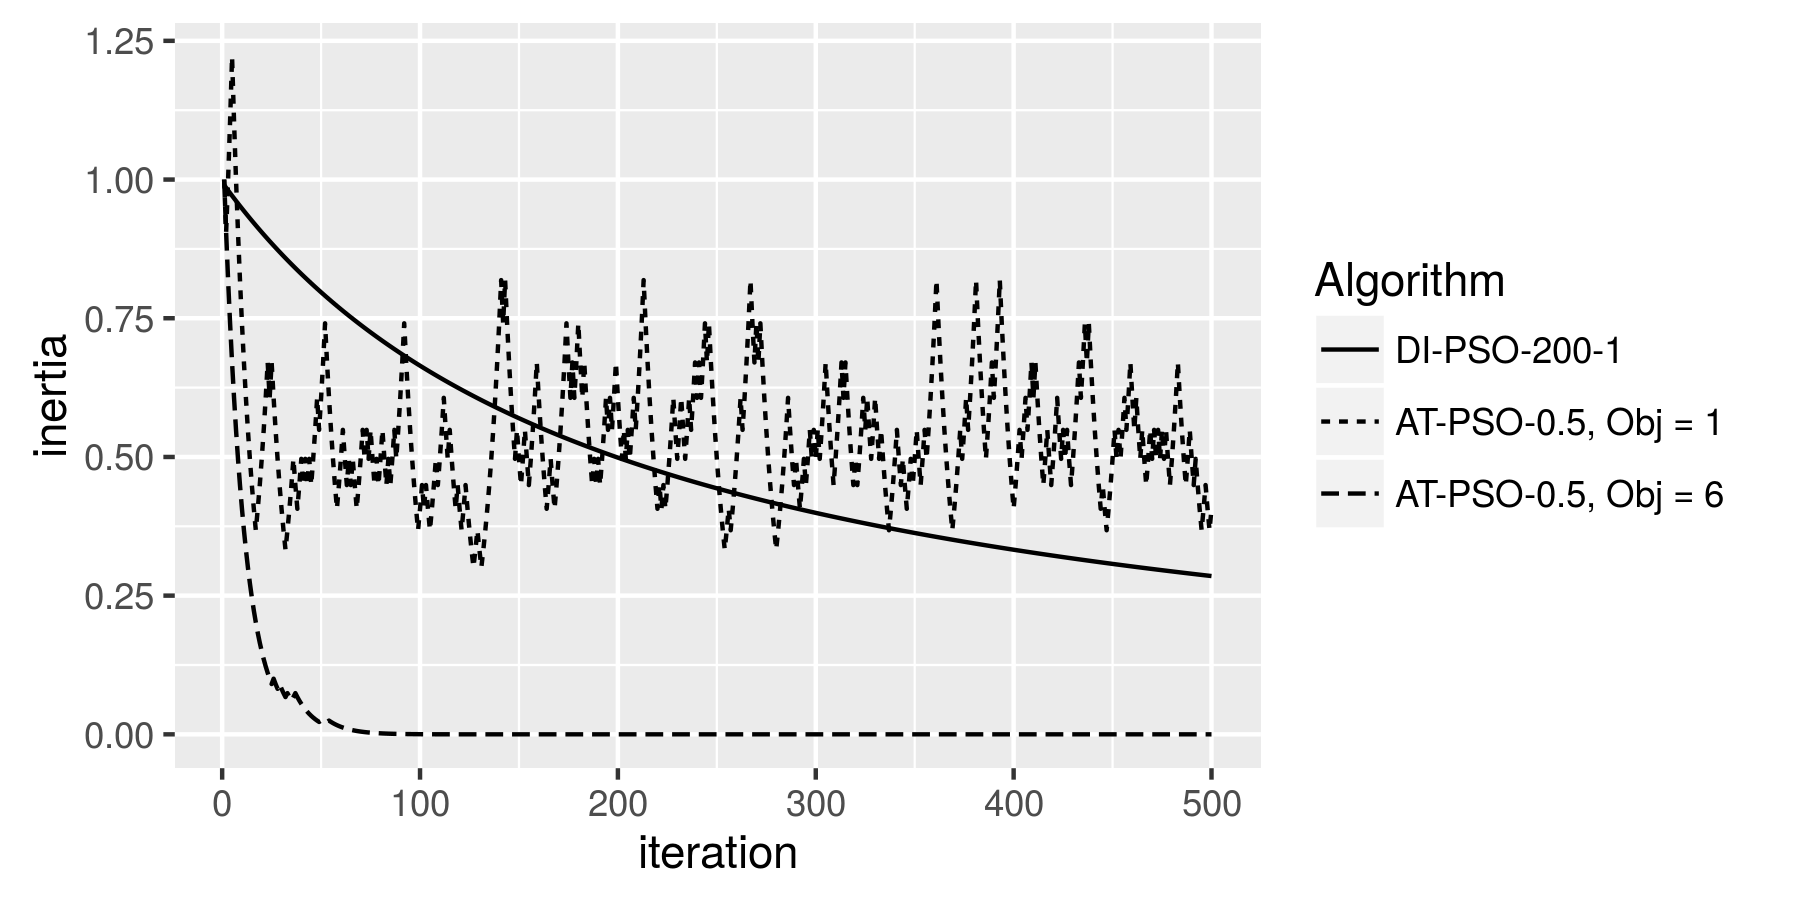
\includegraphics[width=0.95\textwidth]{psosims/inertiaplot.png}
\caption{Inertia over time for the DI-PSO algorithm with $\alpha=200$ and $\beta=1$, and for one replication of the AT-PSO-0.5 algorithm for each of OFs 1 and 6.}
\label{fig:inertia}
\end{figure}


Based on these simulations, our default recommendation is conditional. In problems where convergence is important, such as when finding the posterior mode to use for the normal approximation in a Metropolis proposal, we recommend AT-PSO with $R^*=0.3$ or $0.5$ and using a fairly restricted neighborhood (e.g., ring-1 or ring-3). These algorithms are often the best at meeting convergence criteria, especially in problems with few or no extra local optima. In difficult problems where convergence is less important (e.g., in machine learning) an AT-BBPSO variant with $df=1$ and $R^*=0.3$ or $0.5$, and again with a restrictive neighborhood seems appropriate. These sorts of algorithms seem to do a better job of getting into a region around the global max, though not as well at searching through that region. This bipartite strategy suggests a combined strategy: use AT-BBPSO at first in order to quickly find a good region of the search space then use AT-PSO to quickly search through that region. We do not explore this strategy here, but in Section~\ref{sec:psomode} we find that using BFGS to obtain an initial estimate of the maximum before running any of the PSO algorithms tends to drastically improve the PSO algorithm at a low cost --- at least for the statistical examples considered there.

% latex table generated in R 3.3.1 by xtable 1.8-2 package
% Tue Jun 28 14:37:02 2016
\begin{table}[ht]
\centering
\footnotesize{
\begin{tabular}{r|rrrr|rrrr|rrrr}
\multicolumn{1}{l}{Obj = 1} & \multicolumn{4}{c}{Global nbhd} & \multicolumn{4}{c}{Ring-3 nbhd} & \multicolumn{4}{c}{Ring-1 nbhd}\\
  \hline
Algorithm & Mean & SD & $\widehat{p}_2$ & $\widehat{p}_4$ & Mean & SD & $\widehat{p}_2$ & $\widehat{p}_4$ & Mean & SD & $\widehat{p}_2$ & $\widehat{p}_4$ \\ 
  \hline
\multicolumn{1}{l|}{PSO} & 0.00 & 0.01 & 0.98 & 0.92 & 0.00 & 0.00 & 1.00 & 1.00 & 0.00 & 0.00 & 1.00 & 1.00 \\ 
  \multicolumn{1}{l|}{BBPSO-MC} & 0.12 & 0.04 & 0.00 & 0.00 & 0.09 & 0.03 & 0.00 & 0.00 & 0.04 & 0.02 & 0.06 & 0.00 \\ 
  \multicolumn{1}{l|}{BBPSOxp-MC} & 0.02 & 0.01 & 0.06 & 0.00 & 0.01 & 0.01 & 0.60 & 0.00 & 0.00 & 0.00 & 1.00 & 0.00 \\ 
\hline
\multicolumn{1}{l|}{AT-BBPSO-MC} &&&&&&&&&&&&\\
  $df = 1,\enspace$ $R^* =0.1$ & 0.02 & 0.01 & 0.02 & 0.00 & 0.01 & 0.01 & 0.22 & 0.00 & 0.00 & 0.00 & 0.96 & 0.00 \\ 
  $df = 1,\enspace$ $R^* =0.3$ & 0.02 & 0.01 & 0.06 & 0.00 & 0.01 & 0.00 & 0.22 & 0.00 & 0.00 & 0.00 & 0.96 & 0.00 \\ 
  $df = 1,\enspace$ $R^* =0.5$ & 0.02 & 0.01 & 0.04 & 0.00 & 0.01 & 0.00 & 0.10 & 0.00 & 0.00 & 0.00 & 0.96 & 0.00 \\ 
  $df = 1,\enspace$ $R^* =0.7$ & 0.02 & 0.01 & 0.06 & 0.00 & 0.01 & 0.01 & 0.22 & 0.00 & 0.00 & 0.00 & 0.98 & 0.00 \\ 
  $df = 3,\enspace$ $R^* =0.1$ & 0.04 & 0.01 & 0.02 & 0.00 & 0.03 & 0.01 & 0.00 & 0.00 & 0.01 & 0.00 & 0.70 & 0.00 \\ 
  $df = 3,\enspace$ $R^* =0.3$ & 0.04 & 0.02 & 0.00 & 0.00 & 0.03 & 0.01 & 0.00 & 0.00 & 0.01 & 0.00 & 0.56 & 0.00 \\ 
  $df = 3,\enspace$ $R^* =0.5$ & 0.04 & 0.01 & 0.00 & 0.00 & 0.03 & 0.01 & 0.02 & 0.00 & 0.01 & 0.00 & 0.60 & 0.00 \\ 
  $df = 3,\enspace$ $R^* =0.7$ & 0.04 & 0.01 & 0.00 & 0.00 & 0.03 & 0.01 & 0.02 & 0.00 & 0.01 & 0.00 & 0.64 & 0.00 \\ 
  $df = 5,\enspace$ $R^* =0.1$ & 0.06 & 0.02 & 0.00 & 0.00 & 0.04 & 0.02 & 0.00 & 0.00 & 0.01 & 0.01 & 0.32 & 0.00 \\ 
  $df = 5,\enspace$ $R^* =0.3$ & 0.06 & 0.02 & 0.00 & 0.00 & 0.04 & 0.01 & 0.00 & 0.00 & 0.02 & 0.01 & 0.26 & 0.00 \\ 
  $df = 5,\enspace$ $R^* =0.5$ & 0.06 & 0.02 & 0.00 & 0.00 & 0.04 & 0.01 & 0.00 & 0.00 & 0.01 & 0.01 & 0.34 & 0.00 \\ 
  $df = 5,\enspace$ $R^* =0.7$ & 0.06 & 0.02 & 0.00 & 0.00 & 0.04 & 0.01 & 0.00 & 0.00 & 0.01 & 0.01 & 0.36 & 0.00 \\ 
  $df = \infty,$ $R^* =0.1$ & 0.13 & 0.04 & 0.00 & 0.00 & 0.09 & 0.04 & 0.00 & 0.00 & 0.04 & 0.02 & 0.00 & 0.00 \\ 
  $df = \infty,$ $R^* =0.3$ & 0.12 & 0.04 & 0.00 & 0.00 & 0.09 & 0.02 & 0.00 & 0.00 & 0.04 & 0.02 & 0.02 & 0.00 \\ 
  $df = \infty,$ $R^* =0.5$ & 0.13 & 0.04 & 0.00 & 0.00 & 0.10 & 0.03 & 0.00 & 0.00 & 0.04 & 0.02 & 0.02 & 0.00 \\ 
  $df = \infty,$ $R^* =0.7$ & 0.12 & 0.04 & 0.00 & 0.00 & 0.09 & 0.03 & 0.00 & 0.00 & 0.03 & 0.02 & 0.00 & 0.00 \\ 
\hline
\multicolumn{1}{l|}{AT-BBPSOxp-MC} &&&&&&&&&&&&\\
  $df = 1,\enspace$ $R^* =0.1$ & 0.00 & 0.00 & 0.98 & 0.00 & 0.00 & 0.00 & 1.00 & 0.00 & 0.00 & 0.00 & 1.00 & 0.20 \\ 
  $df = 1,\enspace$ $R^* =0.3$ & 0.00 & 0.00 & 0.98 & 0.00 & 0.00 & 0.00 & 1.00 & 0.00 & 0.00 & 0.00 & 1.00 & 0.32 \\ 
  $df = 1,\enspace$ $R^* =0.5$ & 0.00 & 0.00 & 1.00 & 0.00 & 0.00 & 0.00 & 1.00 & 0.00 & 0.00 & 0.00 & 1.00 & 0.26 \\ 
  $df = 1,\enspace$ $R^* =0.7$ & 0.00 & 0.00 & 1.00 & 0.00 & 0.00 & 0.00 & 1.00 & 0.00 & 0.00 & 0.00 & 1.00 & 0.20 \\ 
  $df = 3,\enspace$ $R^* =0.1$ & 0.01 & 0.00 & 0.90 & 0.00 & 0.00 & 0.00 & 1.00 & 0.00 & 0.00 & 0.00 & 1.00 & 0.10 \\ 
  $df = 3,\enspace$ $R^* =0.3$ & 0.01 & 0.00 & 0.94 & 0.00 & 0.00 & 0.00 & 1.00 & 0.00 & 0.00 & 0.00 & 1.00 & 0.10 \\ 
  $df = 3,\enspace$ $R^* =0.5$ & 0.01 & 0.00 & 0.88 & 0.00 & 0.00 & 0.00 & 1.00 & 0.00 & 0.00 & 0.00 & 1.00 & 0.06 \\ 
  $df = 3,\enspace$ $R^* =0.7$ & 0.01 & 0.00 & 0.90 & 0.00 & 0.00 & 0.00 & 1.00 & 0.00 & 0.00 & 0.00 & 1.00 & 0.08 \\ 
  $df = 5,\enspace$ $R^* =0.1$ & 0.01 & 0.00 & 0.64 & 0.00 & 0.00 & 0.00 & 1.00 & 0.00 & 0.00 & 0.00 & 1.00 & 0.08 \\ 
  $df = 5,\enspace$ $R^* =0.3$ & 0.01 & 0.00 & 0.50 & 0.00 & 0.00 & 0.00 & 0.96 & 0.00 & 0.00 & 0.00 & 1.00 & 0.02 \\ 
  $df = 5,\enspace$ $R^* =0.5$ & 0.01 & 0.00 & 0.58 & 0.00 & 0.00 & 0.00 & 0.98 & 0.00 & 0.00 & 0.00 & 1.00 & 0.02 \\ 
  $df = 5,\enspace$ $R^* =0.7$ & 0.01 & 0.00 & 0.54 & 0.00 & 0.00 & 0.00 & 1.00 & 0.00 & 0.00 & 0.00 & 1.00 & 0.04 \\ 
  $df = \infty,$ $R^* =0.1$ & 0.02 & 0.01 & 0.00 & 0.00 & 0.01 & 0.00 & 0.58 & 0.00 & 0.00 & 0.00 & 1.00 & 0.00 \\ 
  $df = \infty,$ $R^* =0.3$ & 0.02 & 0.01 & 0.06 & 0.00 & 0.01 & 0.00 & 0.52 & 0.00 & 0.00 & 0.00 & 1.00 & 0.02 \\ 
  $df = \infty,$ $R^* =0.5$ & 0.02 & 0.01 & 0.10 & 0.00 & 0.01 & 0.01 & 0.60 & 0.00 & 0.00 & 0.00 & 1.00 & 0.00 \\ 
  $df = \infty,$ $R^* =0.7$ & 0.02 & 0.01 & 0.10 & 0.00 & 0.01 & 0.00 & 0.58 & 0.00 & 0.00 & 0.00 & 1.00 & 0.00 \\ 
\hline
\multicolumn{1}{l|}{DI-PSO} &&&&&&&&&&&&\\
  $\alpha = 50,\enspace$ $\beta =1$ & 54.28 & 103.76 & 0.00 & 0.00 & 0.02 & 0.08 & 0.88 & 0.46 & 0.00 & 0.01 & 0.98 & 0.66 \\ 
  $\alpha = 50,\enspace$ $\beta =2$ & 272.52 & 697.62 & 0.00 & 0.00 & 1.08 & 3.29 & 0.14 & 0.00 & 0.82 & 1.17 & 0.12 & 0.00 \\ 
  $\alpha = 50,\enspace$ $\beta =4$ & 883.23 & 1791.32 & 0.00 & 0.00 & 35.34 & 64.52 & 0.00 & 0.00 & 70.01 & 110.22 & 0.00 & 0.00 \\ 
  $\alpha = 100,$ $\beta =1$ & 3.10 & 7.30 & 0.16 & 0.00 & 0.00 & 0.00 & 1.00 & 0.94 & 0.00 & 0.00 & 1.00 & 1.00 \\ 
  $\alpha = 100,$ $\beta =2$ & 131.33 & 377.01 & 0.00 & 0.00 & 0.35 & 1.31 & 0.72 & 0.28 & 0.01 & 0.03 & 0.90 & 0.20 \\ 
  $\alpha = 100,$ $\beta =4$ & 380.00 & 756.97 & 0.00 & 0.00 & 21.23 & 77.39 & 0.02 & 0.00 & 8.73 & 20.23 & 0.00 & 0.00 \\ 
  $\alpha = 200,$ $\beta =1$ & 15.54 & 77.96 & 0.48 & 0.14 & 0.00 & 0.00 & 1.00 & 1.00 & 0.00 & 0.00 & 1.00 & 1.00 \\ 
  $\alpha = 200,$ $\beta =2$ & 77.09 & 233.84 & 0.10 & 0.00 & 0.00 & 0.00 & 1.00 & 0.88 & 0.00 & 0.00 & 1.00 & 1.00 \\ 
  $\alpha = 200,$ $\beta =4$ & 306.53 & 462.20 & 0.00 & 0.00 & 7.72 & 39.48 & 0.34 & 0.02 & 0.57 & 2.02 & 0.28 & 0.00 \\ 
\hline
\multicolumn{1}{l|}{AT-PSO} &&&&&&&&&&&&\\
  $R^* = 0.1$ & 0.00 & 0.00 & 1.00 & 1.00 & 0.00 & 0.00 & 1.00 & 1.00 & 6.49 & 20.38 & 0.12 & 0.00 \\ 
  $R^* = 0.3$ & 0.00 & 0.00 & 1.00 & 1.00 & 0.00 & 0.00 & 1.00 & 1.00 & 0.00 & 0.00 & 1.00 & 1.00 \\ 
  $R^* = 0.5$ & 0.00 & 0.02 & 0.98 & 0.84 & 0.00 & 0.00 & 1.00 & 1.00 & 0.00 & 0.00 & 1.00 & 1.00 \\ 
  $R^* = 0.7$ & 10.19 & 30.90 & 0.20 & 0.12 & 0.00 & 0.00 & 1.00 & 1.00 & 0.00 & 0.00 & 1.00 & 1.00 \\ 
   \hline
\end{tabular}
}
\caption{Simulation results for OF1 with $D=20$. Each PSO algorithm was initiated in a range that did not contain the true maximum with 20 particles and run for 500 iterations, repeated for 50 repetitions. The Mean and SD columns represent the mean and standard deviation of the difference between the found maximum and the true maximum, while $\widehat{p}_i$ denotes the proportion of the repetitions that ended within $10^{-i}$ of the true maximum for $i=2,4$.}
\label{tab:psosim1}
\end{table}
% latex table generated in R 3.3.1 by xtable 1.8-2 package
% Tue Jun 28 14:37:02 2016
\begin{table}[ht]
\centering
\footnotesize{
\begin{tabular}{r|rrrr|rrrr|rrrr}
\multicolumn{1}{l}{Obj = 2} & \multicolumn{4}{c}{Global nbhd} & \multicolumn{4}{c}{Ring-3 nbhd} & \multicolumn{4}{c}{Ring-1 nbhd}\\
  \hline
Algorithm & Mean & SD & $\widehat{p}_2$ & $\widehat{p}_4$ & Mean & SD & $\widehat{p}_2$ & $\widehat{p}_4$ & Mean & SD & $\widehat{p}_2$ & $\widehat{p}_4$ \\ 
  \hline
\multicolumn{1}{l|}{PSO} & 15.69 & 80.28 & 0.66 & 0.42 & 0.01 & 0.01 & 0.86 & 0.10 & 1.92 & 4.16 & 0.00 & 0.00 \\ 
  \multicolumn{1}{l|}{BBPSO-MC} & 0.43 & 0.13 & 0.00 & 0.00 & 0.47 & 0.23 & 0.00 & 0.00 & 0.72 & 0.53 & 0.00 & 0.00 \\ 
  \multicolumn{1}{l|}{BBPSOxp-MC} & 2.10 & 1.59 & 0.00 & 0.00 & 3.64 & 4.33 & 0.00 & 0.00 & 3.20 & 7.55 & 0.00 & 0.00 \\ 
\hline
\multicolumn{1}{l|}{AT-BBPSO-MC} &&&&&&&&&&&&\\
  $df = 1,\enspace$ $R^* =0.1$ & 0.17 & 0.10 & 0.00 & 0.00 & 0.18 & 0.09 & 0.00 & 0.00 & 0.10 & 0.08 & 0.00 & 0.00 \\ 
  $df = 1,\enspace$ $R^* =0.3$ & 0.19 & 0.08 & 0.00 & 0.00 & 0.17 & 0.09 & 0.00 & 0.00 & 0.10 & 0.06 & 0.00 & 0.00 \\ 
  $df = 1,\enspace$ $R^* =0.5$ & 0.17 & 0.09 & 0.00 & 0.00 & 0.19 & 0.11 & 0.00 & 0.00 & 0.16 & 0.14 & 0.00 & 0.00 \\ 
  $df = 1,\enspace$ $R^* =0.7$ & 0.18 & 0.09 & 0.00 & 0.00 & 0.16 & 0.09 & 0.00 & 0.00 & 0.11 & 0.09 & 0.00 & 0.00 \\ 
  $df = 3,\enspace$ $R^* =0.1$ & 0.20 & 0.08 & 0.00 & 0.00 & 0.18 & 0.10 & 0.00 & 0.00 & 0.17 & 0.17 & 0.00 & 0.00 \\ 
  $df = 3,\enspace$ $R^* =0.3$ & 0.20 & 0.08 & 0.00 & 0.00 & 0.18 & 0.08 & 0.00 & 0.00 & 0.12 & 0.08 & 0.00 & 0.00 \\ 
  $df = 3,\enspace$ $R^* =0.5$ & 0.20 & 0.09 & 0.00 & 0.00 & 0.19 & 0.09 & 0.00 & 0.00 & 0.12 & 0.07 & 0.00 & 0.00 \\ 
  $df = 3,\enspace$ $R^* =0.7$ & 0.21 & 0.08 & 0.00 & 0.00 & 0.22 & 0.08 & 0.00 & 0.00 & 0.12 & 0.10 & 0.00 & 0.00 \\ 
  $df = 5,\enspace$ $R^* =0.1$ & 0.26 & 0.10 & 0.00 & 0.00 & 0.22 & 0.10 & 0.00 & 0.00 & 0.16 & 0.09 & 0.00 & 0.00 \\ 
  $df = 5,\enspace$ $R^* =0.3$ & 0.27 & 0.13 & 0.00 & 0.00 & 0.24 & 0.09 & 0.00 & 0.00 & 0.17 & 0.11 & 0.00 & 0.00 \\ 
  $df = 5,\enspace$ $R^* =0.5$ & 0.25 & 0.08 & 0.00 & 0.00 & 0.24 & 0.10 & 0.00 & 0.00 & 0.16 & 0.10 & 0.00 & 0.00 \\ 
  $df = 5,\enspace$ $R^* =0.7$ & 0.27 & 0.09 & 0.00 & 0.00 & 0.20 & 0.09 & 0.00 & 0.00 & 0.19 & 0.10 & 0.00 & 0.00 \\ 
  $df = \infty,$ $R^* =0.1$ & 0.45 & 0.18 & 0.00 & 0.00 & 0.47 & 0.17 & 0.00 & 0.00 & 0.58 & 0.65 & 0.00 & 0.00 \\ 
  $df = \infty,$ $R^* =0.3$ & 0.52 & 0.22 & 0.00 & 0.00 & 0.46 & 0.20 & 0.00 & 0.00 & 0.57 & 0.38 & 0.00 & 0.00 \\ 
  $df = \infty,$ $R^* =0.5$ & 0.42 & 0.17 & 0.00 & 0.00 & 0.42 & 0.15 & 0.00 & 0.00 & 0.66 & 0.63 & 0.00 & 0.00 \\ 
  $df = \infty,$ $R^* =0.7$ & 0.45 & 0.20 & 0.00 & 0.00 & 0.46 & 0.18 & 0.00 & 0.00 & 0.60 & 0.46 & 0.00 & 0.00 \\ 
\hline
\multicolumn{1}{l|}{AT-BBPSOxp-MC} &&&&&&&&&&&&\\
  $df = 1,\enspace$ $R^* =0.1$ & 1.32 & 0.93 & 0.00 & 0.00 & 0.97 & 0.95 & 0.00 & 0.00 & 0.29 & 0.36 & 0.00 & 0.00 \\ 
  $df = 1,\enspace$ $R^* =0.3$ & 1.33 & 1.25 & 0.00 & 0.00 & 0.98 & 0.86 & 0.00 & 0.00 & 0.23 & 0.26 & 0.00 & 0.00 \\ 
  $df = 1,\enspace$ $R^* =0.5$ & 1.55 & 1.65 & 0.00 & 0.00 & 1.09 & 1.76 & 0.00 & 0.00 & 0.27 & 0.44 & 0.00 & 0.00 \\ 
  $df = 1,\enspace$ $R^* =0.7$ & 1.07 & 0.83 & 0.00 & 0.00 & 1.10 & 1.05 & 0.00 & 0.00 & 0.19 & 0.11 & 0.00 & 0.00 \\ 
  $df = 3,\enspace$ $R^* =0.1$ & 0.72 & 0.56 & 0.00 & 0.00 & 0.69 & 0.50 & 0.00 & 0.00 & 0.29 & 0.24 & 0.00 & 0.00 \\ 
  $df = 3,\enspace$ $R^* =0.3$ & 0.70 & 0.45 & 0.00 & 0.00 & 0.95 & 1.25 & 0.00 & 0.00 & 0.25 & 0.31 & 0.00 & 0.00 \\ 
  $df = 3,\enspace$ $R^* =0.5$ & 0.63 & 0.35 & 0.00 & 0.00 & 0.77 & 0.66 & 0.00 & 0.00 & 0.36 & 0.48 & 0.00 & 0.00 \\ 
  $df = 3,\enspace$ $R^* =0.7$ & 0.64 & 0.49 & 0.00 & 0.00 & 0.73 & 0.47 & 0.00 & 0.00 & 0.32 & 0.42 & 0.00 & 0.00 \\ 
  $df = 5,\enspace$ $R^* =0.1$ & 0.69 & 0.42 & 0.00 & 0.00 & 1.83 & 5.74 & 0.00 & 0.00 & 0.77 & 1.64 & 0.00 & 0.00 \\ 
  $df = 5,\enspace$ $R^* =0.3$ & 0.80 & 0.49 & 0.00 & 0.00 & 0.93 & 0.77 & 0.00 & 0.00 & 0.50 & 0.45 & 0.00 & 0.00 \\ 
  $df = 5,\enspace$ $R^* =0.5$ & 0.99 & 0.79 & 0.00 & 0.00 & 0.83 & 0.69 & 0.00 & 0.00 & 0.73 & 1.06 & 0.00 & 0.00 \\ 
  $df = 5,\enspace$ $R^* =0.7$ & 0.76 & 0.47 & 0.00 & 0.00 & 0.80 & 0.72 & 0.00 & 0.00 & 0.38 & 0.40 & 0.00 & 0.00 \\ 
  $df = \infty,$ $R^* =0.1$ & 2.05 & 1.82 & 0.00 & 0.00 & 4.80 & 6.08 & 0.00 & 0.00 & 4.89 & 8.52 & 0.00 & 0.00 \\ 
  $df = \infty,$ $R^* =0.3$ & 1.53 & 0.80 & 0.00 & 0.00 & 3.90 & 4.95 & 0.00 & 0.00 & 5.17 & 17.76 & 0.00 & 0.00 \\ 
  $df = \infty,$ $R^* =0.5$ & 2.48 & 3.39 & 0.00 & 0.00 & 5.39 & 5.48 & 0.00 & 0.00 & 6.77 & 14.34 & 0.00 & 0.00 \\ 
  $df = \infty,$ $R^* =0.7$ & 2.00 & 1.95 & 0.00 & 0.00 & 4.98 & 7.45 & 0.00 & 0.00 & 5.33 & 10.20 & 0.00 & 0.00 \\ 
\hline
\multicolumn{1}{l|}{DI-PSO} &&&&&&&&&&&&\\
  $\alpha = 50,\enspace$ $\beta =1$ & 1766.75 & 1809.97 & 0.00 & 0.00 & 312.79 & 656.97 & 0.00 & 0.00 & 247.82 & 283.72 & 0.00 & 0.00 \\ 
  $\alpha = 50,\enspace$ $\beta =2$ & 2130.86 & 1542.98 & 0.00 & 0.00 & 748.09 & 740.09 & 0.00 & 0.00 & 710.64 & 654.96 & 0.00 & 0.00 \\ 
  $\alpha = 50,\enspace$ $\beta =4$ & 4033.77 & 3078.76 & 0.00 & 0.00 & 1429.21 & 1150.46 & 0.00 & 0.00 & 1080.86 & 813.64 & 0.00 & 0.00 \\ 
  $\alpha = 100,$ $\beta =1$ & 691.51 & 844.60 & 0.00 & 0.00 & 30.60 & 44.85 & 0.00 & 0.00 & 28.75 & 37.66 & 0.00 & 0.00 \\ 
  $\alpha = 100,$ $\beta =2$ & 1268.37 & 1340.50 & 0.00 & 0.00 & 224.65 & 353.68 & 0.00 & 0.00 & 245.26 & 235.69 & 0.00 & 0.00 \\ 
  $\alpha = 100,$ $\beta =4$ & 3796.32 & 3766.60 & 0.00 & 0.00 & 965.39 & 781.49 & 0.00 & 0.00 & 815.09 & 734.56 & 0.00 & 0.00 \\ 
  $\alpha = 200,$ $\beta =1$ & 183.38 & 296.44 & 0.00 & 0.00 & 1.89 & 8.81 & 0.16 & 0.02 & 3.77 & 5.72 & 0.00 & 0.00 \\ 
  $\alpha = 200,$ $\beta =2$ & 1399.72 & 1907.35 & 0.00 & 0.00 & 46.32 & 67.92 & 0.00 & 0.00 & 62.39 & 78.82 & 0.00 & 0.00 \\ 
  $\alpha = 200,$ $\beta =4$ & 2832.28 & 2340.56 & 0.00 & 0.00 & 504.02 & 469.28 & 0.00 & 0.00 & 434.14 & 387.50 & 0.00 & 0.00 \\ 
\hline
\multicolumn{1}{l|}{AT-PSO} &&&&&&&&&&&&\\
  $R^* = 0.1$ & 0.02 & 0.11 & 0.78 & 0.14 & 0.04 & 0.09 & 0.58 & 0.00 & 272.50 & 538.58 & 0.00 & 0.00 \\ 
  $R^* = 0.3$ & 4.29 & 20.28 & 0.54 & 0.20 & 0.00 & 0.00 & 1.00 & 1.00 & 0.17 & 0.22 & 0.18 & 0.00 \\ 
  $R^* = 0.5$ & 601.56 & 898.19 & 0.00 & 0.00 & 0.00 & 0.00 & 1.00 & 0.72 & 0.20 & 0.36 & 0.16 & 0.00 \\ 
  $R^* = 0.7$ & 1649.00 & 1551.31 & 0.00 & 0.00 & 3.53 & 8.87 & 0.04 & 0.00 & 15.76 & 21.99 & 0.00 & 0.00 \\ 
   \hline
\end{tabular}
}
\caption{Simulation results for OF2 with $D=20$. Each PSO algorithm was initiated in a range that did not contain the true maximum with 20 particles and run for 500 iterations, repeated for 50 repetitions. The Mean and SD columns represent the mean and standard deviation of the difference between the found maximum and the true maximum, while $\widehat{p}_i$ denotes the proportion of the repetitions that ended within $10^{-i}$ of the true maximum for $i=2,4$.}
\label{tab:psosim2}
\end{table}
% latex table generated in R 3.3.1 by xtable 1.8-2 package
% Tue Jun 28 14:37:02 2016
\begin{table}[ht]
\centering
\footnotesize{
\begin{tabular}{r|rrrr|rrrr|rrrr}
\multicolumn{1}{l}{Obj = 3} & \multicolumn{4}{c}{Global nbhd} & \multicolumn{4}{c}{Ring-3 nbhd} & \multicolumn{4}{c}{Ring-1 nbhd}\\
  \hline
Algorithm & Mean & SD & $\widehat{p}_2$ & $\widehat{p}_4$ & Mean & SD & $\widehat{p}_2$ & $\widehat{p}_4$ & Mean & SD & $\widehat{p}_2$ & $\widehat{p}_4$ \\ 
  \hline
\multicolumn{1}{l|}{PSO} & 144.46 & 295.40 & 0.00 & 0.00 & 35.66 & 54.01 & 0.04 & 0.00 & 25.95 & 68.25 & 0.00 & 0.00 \\ 
  \multicolumn{1}{l|}{BBPSO-MC} & 131.31 & 90.51 & 0.00 & 0.00 & 110.19 & 63.02 & 0.00 & 0.00 & 84.45 & 71.65 & 0.00 & 0.00 \\ 
  \multicolumn{1}{l|}{BBPSOxp-MC} & 37.56 & 14.15 & 0.00 & 0.00 & 25.53 & 8.62 & 0.00 & 0.00 & 18.77 & 6.24 & 0.00 & 0.00 \\ 
\hline
\multicolumn{1}{l|}{AT-BBPSO-MC} &&&&&&&&&&&&\\
  $df = 1,\enspace$ $R^* =0.1$ & 111.48 & 250.62 & 0.00 & 0.00 & 53.72 & 43.43 & 0.00 & 0.00 & 110.78 & 165.53 & 0.00 & 0.00 \\ 
  $df = 1,\enspace$ $R^* =0.3$ & 149.32 & 242.67 & 0.00 & 0.00 & 90.41 & 154.44 & 0.00 & 0.00 & 60.90 & 60.45 & 0.00 & 0.00 \\ 
  $df = 1,\enspace$ $R^* =0.5$ & 106.08 & 127.98 & 0.00 & 0.00 & 78.98 & 111.62 & 0.00 & 0.00 & 49.87 & 53.05 & 0.00 & 0.00 \\ 
  $df = 1,\enspace$ $R^* =0.7$ & 120.35 & 187.50 & 0.00 & 0.00 & 79.60 & 107.68 & 0.00 & 0.00 & 83.29 & 126.26 & 0.00 & 0.00 \\ 
  $df = 3,\enspace$ $R^* =0.1$ & 114.66 & 118.03 & 0.00 & 0.00 & 88.22 & 58.20 & 0.00 & 0.00 & 69.83 & 60.08 & 0.00 & 0.00 \\ 
  $df = 3,\enspace$ $R^* =0.3$ & 144.03 & 225.00 & 0.00 & 0.00 & 78.97 & 65.90 & 0.00 & 0.00 & 73.54 & 100.15 & 0.00 & 0.00 \\ 
  $df = 3,\enspace$ $R^* =0.5$ & 121.44 & 127.02 & 0.00 & 0.00 & 79.52 & 71.45 & 0.00 & 0.00 & 57.98 & 48.82 & 0.00 & 0.00 \\ 
  $df = 3,\enspace$ $R^* =0.7$ & 108.30 & 81.33 & 0.00 & 0.00 & 71.77 & 64.65 & 0.00 & 0.00 & 54.11 & 46.59 & 0.00 & 0.00 \\ 
  $df = 5,\enspace$ $R^* =0.1$ & 125.89 & 116.43 & 0.00 & 0.00 & 78.12 & 32.51 & 0.00 & 0.00 & 71.77 & 44.25 & 0.00 & 0.00 \\ 
  $df = 5,\enspace$ $R^* =0.3$ & 108.21 & 69.88 & 0.00 & 0.00 & 94.78 & 44.39 & 0.00 & 0.00 & 67.79 & 65.60 & 0.00 & 0.00 \\ 
  $df = 5,\enspace$ $R^* =0.5$ & 111.18 & 90.71 & 0.00 & 0.00 & 78.14 & 35.93 & 0.00 & 0.00 & 68.41 & 67.38 & 0.00 & 0.00 \\ 
  $df = 5,\enspace$ $R^* =0.7$ & 107.09 & 63.45 & 0.00 & 0.00 & 93.72 & 69.07 & 0.00 & 0.00 & 71.64 & 92.09 & 0.00 & 0.00 \\ 
  $df = \infty,$ $R^* =0.1$ & 126.16 & 71.55 & 0.00 & 0.00 & 99.98 & 25.30 & 0.00 & 0.00 & 68.42 & 43.53 & 0.00 & 0.00 \\ 
  $df = \infty,$ $R^* =0.3$ & 127.38 & 66.15 & 0.00 & 0.00 & 103.96 & 31.69 & 0.00 & 0.00 & 68.21 & 54.76 & 0.00 & 0.00 \\ 
  $df = \infty,$ $R^* =0.5$ & 109.58 & 30.42 & 0.00 & 0.00 & 102.75 & 39.42 & 0.00 & 0.00 & 76.03 & 59.73 & 0.00 & 0.00 \\ 
  $df = \infty,$ $R^* =0.7$ & 112.31 & 31.53 & 0.00 & 0.00 & 111.33 & 47.31 & 0.00 & 0.00 & 72.48 & 29.60 & 0.00 & 0.00 \\ 
\hline
\multicolumn{1}{l|}{AT-BBPSOxp-MC} &&&&&&&&&&&&\\
  $df = 1,\enspace$ $R^* =0.1$ & 54.91 & 71.36 & 0.00 & 0.00 & 46.43 & 53.25 & 0.00 & 0.00 & 27.74 & 33.78 & 0.00 & 0.00 \\ 
  $df = 1,\enspace$ $R^* =0.3$ & 42.75 & 27.54 & 0.00 & 0.00 & 34.70 & 44.52 & 0.00 & 0.00 & 26.56 & 35.25 & 0.00 & 0.00 \\ 
  $df = 1,\enspace$ $R^* =0.5$ & 47.05 & 33.70 & 0.00 & 0.00 & 52.38 & 84.94 & 0.00 & 0.00 & 35.21 & 47.68 & 0.00 & 0.00 \\ 
  $df = 1,\enspace$ $R^* =0.7$ & 44.34 & 44.22 & 0.00 & 0.00 & 55.48 & 108.75 & 0.00 & 0.00 & 39.44 & 46.50 & 0.00 & 0.00 \\ 
  $df = 3,\enspace$ $R^* =0.1$ & 34.88 & 12.52 & 0.00 & 0.00 & 35.55 & 22.20 & 0.00 & 0.00 & 19.04 & 13.27 & 0.00 & 0.00 \\ 
  $df = 3,\enspace$ $R^* =0.3$ & 40.08 & 14.57 & 0.00 & 0.00 & 33.62 & 25.98 & 0.00 & 0.00 & 23.77 & 19.44 & 0.00 & 0.00 \\ 
  $df = 3,\enspace$ $R^* =0.5$ & 44.76 & 48.60 & 0.00 & 0.00 & 27.92 & 12.79 & 0.00 & 0.00 & 27.27 & 35.43 & 0.00 & 0.00 \\ 
  $df = 3,\enspace$ $R^* =0.7$ & 46.32 & 77.32 & 0.00 & 0.00 & 30.46 & 14.12 & 0.00 & 0.00 & 18.80 & 8.33 & 0.00 & 0.00 \\ 
  $df = 5,\enspace$ $R^* =0.1$ & 40.72 & 15.41 & 0.00 & 0.00 & 35.09 & 28.26 & 0.00 & 0.00 & 20.00 & 19.18 & 0.00 & 0.00 \\ 
  $df = 5,\enspace$ $R^* =0.3$ & 40.81 & 22.60 & 0.00 & 0.00 & 32.33 & 19.05 & 0.00 & 0.00 & 20.36 & 12.27 & 0.00 & 0.00 \\ 
  $df = 5,\enspace$ $R^* =0.5$ & 43.59 & 51.50 & 0.00 & 0.00 & 43.91 & 76.14 & 0.00 & 0.00 & 29.54 & 51.03 & 0.00 & 0.00 \\ 
  $df = 5,\enspace$ $R^* =0.7$ & 38.25 & 13.76 & 0.00 & 0.00 & 29.31 & 12.40 & 0.00 & 0.00 & 21.43 & 26.09 & 0.00 & 0.00 \\ 
  $df = \infty,$ $R^* =0.1$ & 40.62 & 19.73 & 0.00 & 0.00 & 31.86 & 18.35 & 0.00 & 0.00 & 25.61 & 42.18 & 0.00 & 0.00 \\ 
  $df = \infty,$ $R^* =0.3$ & 37.54 & 31.58 & 0.00 & 0.00 & 27.73 & 9.34 & 0.00 & 0.00 & 17.79 & 6.45 & 0.00 & 0.00 \\ 
  $df = \infty,$ $R^* =0.5$ & 39.05 & 14.07 & 0.00 & 0.00 & 27.79 & 8.39 & 0.00 & 0.00 & 20.38 & 6.64 & 0.00 & 0.00 \\ 
  $df = \infty,$ $R^* =0.7$ & 35.58 & 12.57 & 0.00 & 0.00 & 28.22 & 8.33 & 0.00 & 0.00 & 18.96 & 7.86 & 0.00 & 0.00 \\ 
\hline
\multicolumn{1}{l|}{DI-PSO} &&&&&&&&&&&&\\
  $\alpha = 50,\enspace$ $\beta =1$ & 1349.13 & 1940.53 & 0.00 & 0.00 & 200.09 & 245.80 & 0.00 & 0.00 & 149.74 & 221.74 & 0.00 & 0.00 \\ 
  $\alpha = 50,\enspace$ $\beta =2$ & 7204.93 & 16333.63 & 0.00 & 0.00 & 785.95 & 2896.36 & 0.00 & 0.00 & 339.44 & 446.58 & 0.00 & 0.00 \\ 
  $\alpha = 50,\enspace$ $\beta =4$ & 24307.11 & 42723.81 & 0.00 & 0.00 & 7881.86 & 26566.77 & 0.00 & 0.00 & 19136.28 & 43990.37 & 0.00 & 0.00 \\ 
  $\alpha = 100,$ $\beta =1$ & 420.14 & 827.79 & 0.00 & 0.00 & 108.58 & 211.14 & 0.00 & 0.00 & 78.35 & 107.85 & 0.00 & 0.00 \\ 
  $\alpha = 100,$ $\beta =2$ & 1245.63 & 1717.55 & 0.00 & 0.00 & 653.55 & 2182.72 & 0.00 & 0.00 & 214.47 & 545.19 & 0.00 & 0.00 \\ 
  $\alpha = 100,$ $\beta =4$ & 33664.67 & 97150.26 & 0.00 & 0.00 & 1398.23 & 2729.87 & 0.00 & 0.00 & 2100.05 & 4701.80 & 0.00 & 0.00 \\ 
  $\alpha = 200,$ $\beta =1$ & 636.50 & 1081.78 & 0.00 & 0.00 & 101.35 & 197.94 & 0.00 & 0.00 & 52.42 & 71.41 & 0.02 & 0.00 \\ 
  $\alpha = 200,$ $\beta =2$ & 1013.55 & 2221.85 & 0.00 & 0.00 & 237.69 & 524.60 & 0.00 & 0.00 & 144.29 & 270.95 & 0.00 & 0.00 \\ 
  $\alpha = 200,$ $\beta =4$ & 12140.28 & 30312.75 & 0.00 & 0.00 & 3804.18 & 20640.37 & 0.00 & 0.00 & 1031.02 & 2712.71 & 0.00 & 0.00 \\ 
\hline
\multicolumn{1}{l|}{AT-PSO} &&&&&&&&&&&&\\
  $R^* = 0.1$ & 76.28 & 161.98 & 0.00 & 0.00 & 92.06 & 184.12 & 0.00 & 0.00 & 3963.70 & 12776.53 & 0.00 & 0.00 \\ 
  $R^* = 0.3$ & 132.79 & 162.86 & 0.00 & 0.00 & 50.07 & 101.57 & 0.00 & 0.00 & 61.91 & 139.04 & 0.00 & 0.00 \\ 
  $R^* = 0.5$ & 239.14 & 413.19 & 0.00 & 0.00 & 79.24 & 139.68 & 0.00 & 0.00 & 48.67 & 81.20 & 0.02 & 0.02 \\ 
  $R^* = 0.7$ & 673.23 & 1512.39 & 0.00 & 0.00 & 86.14 & 193.93 & 0.00 & 0.00 & 90.40 & 117.98 & 0.00 & 0.00 \\ 
   \hline
\end{tabular}
}
\caption{Simulation results for OF3 with $D=20$. Each PSO algorithm was initiated in a range that did not contain the true maximum with 20 particles and run for 500 iterations, repeated for 50 repetitions. The Mean and SD columns represent the mean and standard deviation of the difference between the found maximum and the true maximum, while $\widehat{p}_i$ denotes the proportion of the repetitions that ended within $10^{-i}$ of the true maximum for $i=2,4$.}
\label{tab:psosim3}
\end{table}
% latex table generated in R 3.3.1 by xtable 1.8-2 package
% Tue Jun 28 14:37:02 2016
\begin{table}[ht]
\centering
\footnotesize{
\begin{tabular}{r|rrrr|rrrr|rrrr}
\multicolumn{1}{l}{Obj = 4} & \multicolumn{4}{c}{Global nbhd} & \multicolumn{4}{c}{Ring-3 nbhd} & \multicolumn{4}{c}{Ring-1 nbhd}\\
  \hline
Algorithm & Mean & SD & $\widehat{p}_2$ & $\widehat{p}_4$ & Mean & SD & $\widehat{p}_2$ & $\widehat{p}_4$ & Mean & SD & $\widehat{p}_2$ & $\widehat{p}_4$ \\ 
  \hline
\multicolumn{1}{l|}{PSO} & 4.32 & 2.75 & 0.02 & 0.02 & 0.65 & 0.89 & 0.56 & 0.56 & 0.13 & 0.47 & 0.90 & 0.86 \\ 
  \multicolumn{1}{l|}{BBPSO-MC} & 2.75 & 0.93 & 0.00 & 0.00 & 2.67 & 0.81 & 0.00 & 0.00 & 1.47 & 1.00 & 0.00 & 0.00 \\ 
  \multicolumn{1}{l|}{BBPSOxp-MC} & 0.13 & 0.05 & 0.00 & 0.00 & 0.04 & 0.02 & 0.04 & 0.00 & 0.01 & 0.00 & 0.86 & 0.00 \\ 
\hline
\multicolumn{1}{l|}{AT-BBPSO-MC} &&&&&&&&&&&&\\
  $df = 1,\enspace$ $R^* =0.1$ & 1.02 & 0.80 & 0.00 & 0.00 & 0.48 & 0.38 & 0.00 & 0.00 & 0.21 & 0.23 & 0.00 & 0.00 \\ 
  $df = 1,\enspace$ $R^* =0.3$ & 1.10 & 0.88 & 0.00 & 0.00 & 0.58 & 0.39 & 0.00 & 0.00 & 0.23 & 0.28 & 0.00 & 0.00 \\ 
  $df = 1,\enspace$ $R^* =0.5$ & 0.90 & 0.66 & 0.00 & 0.00 & 0.51 & 0.33 & 0.00 & 0.00 & 0.37 & 0.42 & 0.00 & 0.00 \\ 
  $df = 1,\enspace$ $R^* =0.7$ & 0.98 & 0.68 & 0.00 & 0.00 & 0.50 & 0.31 & 0.00 & 0.00 & 0.29 & 0.43 & 0.00 & 0.00 \\ 
  $df = 3,\enspace$ $R^* =0.1$ & 1.13 & 0.56 & 0.00 & 0.00 & 0.91 & 0.42 & 0.00 & 0.00 & 0.47 & 0.48 & 0.00 & 0.00 \\ 
  $df = 3,\enspace$ $R^* =0.3$ & 1.25 & 0.54 & 0.00 & 0.00 & 0.89 & 0.52 & 0.00 & 0.00 & 0.46 & 0.48 & 0.00 & 0.00 \\ 
  $df = 3,\enspace$ $R^* =0.5$ & 1.23 & 0.48 & 0.00 & 0.00 & 0.97 & 0.48 & 0.00 & 0.00 & 0.40 & 0.47 & 0.00 & 0.00 \\ 
  $df = 3,\enspace$ $R^* =0.7$ & 1.25 & 0.63 & 0.00 & 0.00 & 1.05 & 0.64 & 0.00 & 0.00 & 0.40 & 0.45 & 0.00 & 0.00 \\ 
  $df = 5,\enspace$ $R^* =0.1$ & 1.54 & 0.64 & 0.00 & 0.00 & 1.25 & 0.53 & 0.00 & 0.00 & 0.81 & 0.62 & 0.00 & 0.00 \\ 
  $df = 5,\enspace$ $R^* =0.3$ & 1.64 & 0.48 & 0.00 & 0.00 & 1.38 & 0.63 & 0.00 & 0.00 & 0.53 & 0.49 & 0.00 & 0.00 \\ 
  $df = 5,\enspace$ $R^* =0.5$ & 1.72 & 0.60 & 0.00 & 0.00 & 1.59 & 0.77 & 0.00 & 0.00 & 0.55 & 0.47 & 0.00 & 0.00 \\ 
  $df = 5,\enspace$ $R^* =0.7$ & 1.77 & 0.66 & 0.00 & 0.00 & 1.30 & 0.67 & 0.00 & 0.00 & 0.53 & 0.43 & 0.00 & 0.00 \\ 
  $df = \infty,$ $R^* =0.1$ & 2.63 & 0.78 & 0.00 & 0.00 & 2.42 & 0.86 & 0.00 & 0.00 & 1.38 & 0.86 & 0.00 & 0.00 \\ 
  $df = \infty,$ $R^* =0.3$ & 2.52 & 0.63 & 0.00 & 0.00 & 2.51 & 0.58 & 0.00 & 0.00 & 1.22 & 0.76 & 0.00 & 0.00 \\ 
  $df = \infty,$ $R^* =0.5$ & 2.50 & 0.84 & 0.00 & 0.00 & 2.40 & 0.77 & 0.00 & 0.00 & 1.49 & 0.90 & 0.00 & 0.00 \\ 
  $df = \infty,$ $R^* =0.7$ & 2.63 & 0.66 & 0.00 & 0.00 & 2.62 & 0.72 & 0.00 & 0.00 & 1.34 & 0.95 & 0.00 & 0.00 \\ 
\hline
\multicolumn{1}{l|}{AT-BBPSOxp-MC} &&&&&&&&&&&&\\
  $df = 1,\enspace$ $R^* =0.1$ & 0.09 & 0.04 & 0.00 & 0.00 & 0.02 & 0.01 & 0.06 & 0.00 & 0.00 & 0.00 & 1.00 & 0.00 \\ 
  $df = 1,\enspace$ $R^* =0.3$ & 0.08 & 0.04 & 0.00 & 0.00 & 0.03 & 0.01 & 0.02 & 0.00 & 0.00 & 0.00 & 0.94 & 0.00 \\ 
  $df = 1,\enspace$ $R^* =0.5$ & 0.07 & 0.03 & 0.00 & 0.00 & 0.03 & 0.01 & 0.10 & 0.00 & 0.00 & 0.00 & 0.94 & 0.00 \\ 
  $df = 1,\enspace$ $R^* =0.7$ & 0.07 & 0.03 & 0.00 & 0.00 & 0.03 & 0.01 & 0.04 & 0.00 & 0.00 & 0.00 & 1.00 & 0.00 \\ 
  $df = 3,\enspace$ $R^* =0.1$ & 0.10 & 0.04 & 0.00 & 0.00 & 0.03 & 0.01 & 0.02 & 0.00 & 0.00 & 0.00 & 0.98 & 0.00 \\ 
  $df = 3,\enspace$ $R^* =0.3$ & 0.10 & 0.04 & 0.00 & 0.00 & 0.03 & 0.01 & 0.02 & 0.00 & 0.00 & 0.00 & 0.98 & 0.00 \\ 
  $df = 3,\enspace$ $R^* =0.5$ & 0.10 & 0.04 & 0.00 & 0.00 & 0.03 & 0.01 & 0.00 & 0.00 & 0.00 & 0.00 & 1.00 & 0.00 \\ 
  $df = 3,\enspace$ $R^* =0.7$ & 0.09 & 0.04 & 0.00 & 0.00 & 0.03 & 0.02 & 0.06 & 0.00 & 0.00 & 0.00 & 0.96 & 0.00 \\ 
  $df = 5,\enspace$ $R^* =0.1$ & 0.11 & 0.04 & 0.00 & 0.00 & 0.03 & 0.02 & 0.02 & 0.00 & 0.00 & 0.00 & 0.90 & 0.00 \\ 
  $df = 5,\enspace$ $R^* =0.3$ & 0.10 & 0.04 & 0.00 & 0.00 & 0.03 & 0.01 & 0.00 & 0.00 & 0.00 & 0.00 & 0.96 & 0.00 \\ 
  $df = 5,\enspace$ $R^* =0.5$ & 0.11 & 0.05 & 0.00 & 0.00 & 0.03 & 0.01 & 0.00 & 0.00 & 0.00 & 0.00 & 0.98 & 0.00 \\ 
  $df = 5,\enspace$ $R^* =0.7$ & 0.10 & 0.04 & 0.00 & 0.00 & 0.03 & 0.02 & 0.02 & 0.00 & 0.00 & 0.00 & 0.94 & 0.00 \\ 
  $df = \infty,$ $R^* =0.1$ & 0.12 & 0.05 & 0.00 & 0.00 & 0.04 & 0.02 & 0.00 & 0.00 & 0.00 & 0.00 & 0.98 & 0.02 \\ 
  $df = \infty,$ $R^* =0.3$ & 0.12 & 0.05 & 0.00 & 0.00 & 0.04 & 0.02 & 0.00 & 0.00 & 0.01 & 0.00 & 0.84 & 0.00 \\ 
  $df = \infty,$ $R^* =0.5$ & 0.13 & 0.05 & 0.00 & 0.00 & 0.04 & 0.02 & 0.00 & 0.00 & 0.01 & 0.00 & 0.86 & 0.00 \\ 
  $df = \infty,$ $R^* =0.7$ & 0.12 & 0.04 & 0.00 & 0.00 & 0.04 & 0.02 & 0.00 & 0.00 & 0.00 & 0.00 & 0.94 & 0.00 \\ 
\hline
\multicolumn{1}{l|}{DI-PSO} &&&&&&&&&&&&\\
  $\alpha = 50,\enspace$ $\beta =1$ & 4.42 & 2.42 & 0.00 & 0.00 & 1.35 & 1.07 & 0.24 & 0.12 & 0.63 & 0.89 & 0.50 & 0.26 \\ 
  $\alpha = 50,\enspace$ $\beta =2$ & 4.31 & 2.95 & 0.00 & 0.00 & 1.79 & 1.31 & 0.02 & 0.00 & 0.83 & 0.85 & 0.20 & 0.02 \\ 
  $\alpha = 50,\enspace$ $\beta =4$ & 5.98 & 3.60 & 0.00 & 0.00 & 2.38 & 1.56 & 0.00 & 0.00 & 1.49 & 1.41 & 0.04 & 0.00 \\ 
  $\alpha = 100,$ $\beta =1$ & 2.57 & 2.02 & 0.02 & 0.00 & 1.08 & 1.07 & 0.32 & 0.26 & 0.32 & 0.49 & 0.68 & 0.68 \\ 
  $\alpha = 100,$ $\beta =2$ & 4.15 & 2.84 & 0.00 & 0.00 & 1.63 & 1.26 & 0.16 & 0.04 & 0.43 & 0.90 & 0.56 & 0.14 \\ 
  $\alpha = 100,$ $\beta =4$ & 5.21 & 3.46 & 0.00 & 0.00 & 2.12 & 1.67 & 0.00 & 0.00 & 1.16 & 1.19 & 0.08 & 0.00 \\ 
  $\alpha = 200,$ $\beta =1$ & 1.51 & 1.04 & 0.16 & 0.08 & 0.93 & 0.78 & 0.30 & 0.30 & 0.29 & 0.73 & 0.80 & 0.78 \\ 
  $\alpha = 200,$ $\beta =2$ & 4.21 & 3.29 & 0.02 & 0.00 & 1.29 & 0.88 & 0.12 & 0.12 & 0.46 & 0.62 & 0.60 & 0.48 \\ 
  $\alpha = 200,$ $\beta =4$ & 4.73 & 3.22 & 0.00 & 0.00 & 1.91 & 1.45 & 0.10 & 0.00 & 0.95 & 1.04 & 0.30 & 0.00 \\ 
\hline
\multicolumn{1}{l|}{AT-PSO} &&&&&&&&&&&&\\
  $R^* = 0.1$ & 1.60 & 1.27 & 0.18 & 0.16 & 0.30 & 0.49 & 0.70 & 0.70 & 0.39 & 0.74 & 0.30 & 0.06 \\ 
  $R^* = 0.3$ & 3.80 & 2.65 & 0.02 & 0.02 & 1.18 & 1.15 & 0.38 & 0.38 & 0.27 & 0.43 & 0.72 & 0.72 \\ 
  $R^* = 0.5$ & 6.15 & 4.25 & 0.00 & 0.00 & 2.42 & 2.62 & 0.08 & 0.08 & 1.01 & 1.16 & 0.34 & 0.34 \\ 
  $R^* = 0.7$ & 7.73 & 5.24 & 0.00 & 0.00 & 3.02 & 2.12 & 0.08 & 0.08 & 3.48 & 3.53 & 0.04 & 0.04 \\ 
   \hline
\end{tabular}
}
\caption{Simulation results for OF4 with $D=20$. Each PSO algorithm was initiated in a range that did not contain the true maximum with 20 particles and run for 500 iterations, repeated for 50 repetitions. The Mean and SD columns represent the mean and standard deviation of the difference between the found maximum and the true maximum, while $\widehat{p}_i$ denotes the proportion of the repetitions that ended within $10^{-i}$ of the true maximum for $i=2,4$.}
\label{tab:psosim4}
\end{table}
% latex table generated in R 3.3.1 by xtable 1.8-2 package
% Tue Jun 28 14:37:02 2016
\begin{table}[ht]
\centering
\footnotesize{
\begin{tabular}{r|rrrr|rrrr|rrrr}
\multicolumn{1}{l}{Obj = 5} & \multicolumn{4}{c}{Global nbhd} & \multicolumn{4}{c}{Ring-3 nbhd} & \multicolumn{4}{c}{Ring-1 nbhd}\\
  \hline
Algorithm & Mean & SD & $\widehat{p}_2$ & $\widehat{p}_4$ & Mean & SD & $\widehat{p}_2$ & $\widehat{p}_4$ & Mean & SD & $\widehat{p}_2$ & $\widehat{p}_4$ \\ 
  \hline
\multicolumn{1}{l|}{PSO} & 0.18 & 0.17 & 0.00 & 0.00 & 0.07 & 0.04 & 0.06 & 0.02 & 0.06 & 0.04 & 0.04 & 0.02 \\ 
  \multicolumn{1}{l|}{BBPSO-MC} & 107.55 & 12.45 & 0.00 & 0.00 & 123.72 & 13.02 & 0.00 & 0.00 & 139.39 & 20.19 & 0.00 & 0.00 \\ 
  \multicolumn{1}{l|}{BBPSOxp-MC} & 161.19 & 16.06 & 0.00 & 0.00 & 147.39 & 15.95 & 0.00 & 0.00 & 88.54 & 22.99 & 0.00 & 0.00 \\ 
\hline
\multicolumn{1}{l|}{AT-BBPSO-MC} &&&&&&&&&&&&\\
  $df = 1,\enspace$ $R^* =0.1$ & 0.24 & 0.20 & 0.00 & 0.00 & 0.11 & 0.06 & 0.00 & 0.00 & 0.10 & 0.06 & 0.00 & 0.00 \\ 
  $df = 1,\enspace$ $R^* =0.3$ & 0.22 & 0.15 & 0.00 & 0.00 & 0.14 & 0.08 & 0.00 & 0.00 & 0.10 & 0.08 & 0.02 & 0.00 \\ 
  $df = 1,\enspace$ $R^* =0.5$ & 0.23 & 0.14 & 0.00 & 0.00 & 0.12 & 0.09 & 0.00 & 0.00 & 0.10 & 0.05 & 0.00 & 0.00 \\ 
  $df = 1,\enspace$ $R^* =0.7$ & 0.24 & 0.16 & 0.00 & 0.00 & 0.13 & 0.09 & 0.00 & 0.00 & 0.09 & 0.05 & 0.00 & 0.00 \\ 
  $df = 3,\enspace$ $R^* =0.1$ & 0.75 & 0.61 & 0.00 & 0.00 & 0.29 & 0.18 & 0.00 & 0.00 & 0.50 & 0.34 & 0.00 & 0.00 \\ 
  $df = 3,\enspace$ $R^* =0.3$ & 0.78 & 0.59 & 0.00 & 0.00 & 0.26 & 0.15 & 0.00 & 0.00 & 0.61 & 0.37 & 0.00 & 0.00 \\ 
  $df = 3,\enspace$ $R^* =0.5$ & 0.59 & 0.41 & 0.00 & 0.00 & 0.27 & 0.17 & 0.00 & 0.00 & 0.51 & 0.31 & 0.00 & 0.00 \\ 
  $df = 3,\enspace$ $R^* =0.7$ & 0.64 & 0.45 & 0.00 & 0.00 & 0.28 & 0.15 & 0.00 & 0.00 & 0.57 & 0.40 & 0.00 & 0.00 \\ 
  $df = 5,\enspace$ $R^* =0.1$ & 7.13 & 3.33 & 0.00 & 0.00 & 16.46 & 5.52 & 0.00 & 0.00 & 33.67 & 9.42 & 0.00 & 0.00 \\ 
  $df = 5,\enspace$ $R^* =0.3$ & 8.03 & 3.84 & 0.00 & 0.00 & 16.27 & 4.90 & 0.00 & 0.00 & 31.74 & 9.31 & 0.00 & 0.00 \\ 
  $df = 5,\enspace$ $R^* =0.5$ & 7.18 & 4.05 & 0.00 & 0.00 & 16.78 & 5.88 & 0.00 & 0.00 & 36.30 & 12.42 & 0.00 & 0.00 \\ 
  $df = 5,\enspace$ $R^* =0.7$ & 7.62 & 3.58 & 0.00 & 0.00 & 15.76 & 5.55 & 0.00 & 0.00 & 32.13 & 9.37 & 0.00 & 0.00 \\ 
  $df = \infty,$ $R^* =0.1$ & 108.04 & 13.07 & 0.00 & 0.00 & 122.56 & 10.67 & 0.00 & 0.00 & 138.20 & 17.14 & 0.00 & 0.00 \\ 
  $df = \infty,$ $R^* =0.3$ & 109.07 & 12.30 & 0.00 & 0.00 & 123.46 & 10.82 & 0.00 & 0.00 & 137.72 & 19.34 & 0.00 & 0.00 \\ 
  $df = \infty,$ $R^* =0.5$ & 108.41 & 13.09 & 0.00 & 0.00 & 124.54 & 11.65 & 0.00 & 0.00 & 137.44 & 19.45 & 0.00 & 0.00 \\ 
  $df = \infty,$ $R^* =0.7$ & 108.26 & 12.55 & 0.00 & 0.00 & 125.60 & 10.86 & 0.00 & 0.00 & 138.92 & 19.62 & 0.00 & 0.00 \\ 
\hline
\multicolumn{1}{l|}{AT-BBPSOxp-MC} &&&&&&&&&&&&\\
  $df = 1,\enspace$ $R^* =0.1$ & 0.09 & 0.04 & 0.00 & 0.00 & 0.08 & 0.04 & 0.00 & 0.00 & 0.05 & 0.04 & 0.02 & 0.00 \\ 
  $df = 1,\enspace$ $R^* =0.3$ & 0.10 & 0.05 & 0.00 & 0.00 & 0.08 & 0.05 & 0.06 & 0.00 & 0.06 & 0.03 & 0.02 & 0.00 \\ 
  $df = 1,\enspace$ $R^* =0.5$ & 0.10 & 0.06 & 0.00 & 0.00 & 0.08 & 0.05 & 0.00 & 0.00 & 0.07 & 0.03 & 0.02 & 0.00 \\ 
  $df = 1,\enspace$ $R^* =0.7$ & 0.10 & 0.06 & 0.00 & 0.00 & 0.08 & 0.05 & 0.00 & 0.00 & 0.06 & 0.04 & 0.06 & 0.00 \\ 
  $df = 3,\enspace$ $R^* =0.1$ & 3.37 & 2.43 & 0.00 & 0.00 & 4.40 & 2.86 & 0.00 & 0.00 & 0.90 & 0.87 & 0.00 & 0.00 \\ 
  $df = 3,\enspace$ $R^* =0.3$ & 3.18 & 2.42 & 0.00 & 0.00 & 3.26 & 1.80 & 0.00 & 0.00 & 1.10 & 1.16 & 0.00 & 0.00 \\ 
  $df = 3,\enspace$ $R^* =0.5$ & 3.27 & 2.30 & 0.00 & 0.00 & 3.59 & 3.42 & 0.00 & 0.00 & 0.97 & 1.20 & 0.00 & 0.00 \\ 
  $df = 3,\enspace$ $R^* =0.7$ & 3.71 & 2.43 & 0.00 & 0.00 & 4.97 & 4.03 & 0.00 & 0.00 & 0.83 & 0.70 & 0.00 & 0.00 \\ 
  $df = 5,\enspace$ $R^* =0.1$ & 64.33 & 10.31 & 0.00 & 0.00 & 62.16 & 10.89 & 0.00 & 0.00 & 25.49 & 10.74 & 0.00 & 0.00 \\ 
  $df = 5,\enspace$ $R^* =0.3$ & 63.62 & 10.26 & 0.00 & 0.00 & 61.79 & 12.09 & 0.00 & 0.00 & 26.34 & 10.67 & 0.00 & 0.00 \\ 
  $df = 5,\enspace$ $R^* =0.5$ & 62.01 & 10.94 & 0.00 & 0.00 & 62.58 & 9.87 & 0.00 & 0.00 & 26.15 & 13.04 & 0.00 & 0.00 \\ 
  $df = 5,\enspace$ $R^* =0.7$ & 64.75 & 10.55 & 0.00 & 0.00 & 62.63 & 11.46 & 0.00 & 0.00 & 25.45 & 10.98 & 0.00 & 0.00 \\ 
  $df = \infty,$ $R^* =0.1$ & 157.62 & 14.20 & 0.00 & 0.00 & 148.31 & 13.62 & 0.00 & 0.00 & 87.94 & 24.29 & 0.00 & 0.00 \\ 
  $df = \infty,$ $R^* =0.3$ & 160.30 & 15.23 & 0.00 & 0.00 & 146.65 & 16.52 & 0.00 & 0.00 & 87.96 & 23.07 & 0.00 & 0.00 \\ 
  $df = \infty,$ $R^* =0.5$ & 158.78 & 16.14 & 0.00 & 0.00 & 150.94 & 14.95 & 0.00 & 0.00 & 91.44 & 21.82 & 0.00 & 0.00 \\ 
  $df = \infty,$ $R^* =0.7$ & 162.49 & 16.45 & 0.00 & 0.00 & 145.00 & 16.78 & 0.00 & 0.00 & 87.56 & 20.07 & 0.00 & 0.00 \\ 
\hline
\multicolumn{1}{l|}{DI-PSO} &&&&&&&&&&&&\\
  $\alpha = 50,\enspace$ $\beta =1$ & 1.68 & 3.09 & 0.00 & 0.00 & 0.11 & 0.06 & 0.00 & 0.00 & 0.15 & 0.10 & 0.00 & 0.00 \\ 
  $\alpha = 50,\enspace$ $\beta =2$ & 1.69 & 4.30 & 0.00 & 0.00 & 0.27 & 0.33 & 0.00 & 0.00 & 0.25 & 0.13 & 0.00 & 0.00 \\ 
  $\alpha = 50,\enspace$ $\beta =4$ & 5.70 & 6.13 & 0.00 & 0.00 & 0.79 & 0.95 & 0.00 & 0.00 & 1.01 & 1.23 & 0.00 & 0.00 \\ 
  $\alpha = 100,$ $\beta =1$ & 0.53 & 1.14 & 0.00 & 0.00 & 0.08 & 0.07 & 0.06 & 0.02 & 0.09 & 0.05 & 0.00 & 0.00 \\ 
  $\alpha = 100,$ $\beta =2$ & 2.31 & 4.78 & 0.00 & 0.00 & 0.12 & 0.06 & 0.00 & 0.00 & 0.19 & 0.12 & 0.00 & 0.00 \\ 
  $\alpha = 100,$ $\beta =4$ & 5.42 & 5.89 & 0.00 & 0.00 & 0.39 & 0.39 & 0.00 & 0.00 & 0.40 & 0.27 & 0.00 & 0.00 \\ 
  $\alpha = 200,$ $\beta =1$ & 0.18 & 0.17 & 0.02 & 0.00 & 0.09 & 0.06 & 0.00 & 0.00 & 0.09 & 0.04 & 0.00 & 0.00 \\ 
  $\alpha = 200,$ $\beta =2$ & 0.78 & 1.52 & 0.00 & 0.00 & 0.10 & 0.07 & 0.00 & 0.00 & 0.12 & 0.09 & 0.00 & 0.00 \\ 
  $\alpha = 200,$ $\beta =4$ & 4.33 & 6.70 & 0.00 & 0.00 & 0.24 & 0.17 & 0.00 & 0.00 & 0.25 & 0.12 & 0.00 & 0.00 \\ 
\hline
\multicolumn{1}{l|}{AT-PSO} &&&&&&&&&&&&\\
  $R^* = 0.1$ & 0.11 & 0.08 & 0.00 & 0.00 & 0.07 & 0.03 & 0.00 & 0.00 & 0.38 & 0.30 & 0.00 & 0.00 \\ 
  $R^* = 0.3$ & 0.16 & 0.12 & 0.04 & 0.00 & 0.07 & 0.04 & 0.02 & 0.00 & 0.05 & 0.04 & 0.06 & 0.04 \\ 
  $R^* = 0.5$ & 0.65 & 1.02 & 0.00 & 0.00 & 0.08 & 0.05 & 0.04 & 0.00 & 0.05 & 0.03 & 0.06 & 0.00 \\ 
  $R^* = 0.7$ & 2.50 & 4.89 & 0.00 & 0.00 & 0.23 & 0.21 & 0.00 & 0.00 & 0.21 & 0.20 & 0.00 & 0.00 \\ 
   \hline
\end{tabular}
}
\caption{Simulation results for OF5 with $D=20$. Each PSO algorithm was initiated in a range that did not contain the true maximum with 20 particles and run for 500 iterations, repeated for 50 repetitions. The Mean and SD columns represent the mean and standard deviation of the difference between the found maximum and the true maximum, while $\widehat{p}_i$ denotes the proportion of the repetitions that ended within $10^{-i}$ of the true maximum for $i=2,4$.}
\label{tab:psosim5}
\end{table}
% latex table generated in R 3.3.1 by xtable 1.8-2 package
% Tue Jun 28 14:37:02 2016
\begin{table}[ht]
\centering
\footnotesize{
\begin{tabular}{r|rrrr|rrrr|rrrr}
\multicolumn{1}{l}{Obj = 6} & \multicolumn{4}{c}{Global nbhd} & \multicolumn{4}{c}{Ring-3 nbhd} & \multicolumn{4}{c}{Ring-1 nbhd}\\
  \hline
Algorithm & Mean & SD & $\widehat{p}_2$ & $\widehat{p}_4$ & Mean & SD & $\widehat{p}_2$ & $\widehat{p}_4$ & Mean & SD & $\widehat{p}_2$ & $\widehat{p}_4$ \\ 
  \hline
\multicolumn{1}{l|}{PSO} & 18.95 & 3.04 & 0.02 & 0.02 & 9.06 & 9.92 & 0.54 & 0.50 & 13.43 & 9.17 & 0.24 & 0.08 \\ 
  \multicolumn{1}{l|}{BBPSO-MC} & 20.25 & 0.10 & 0.00 & 0.00 & 20.28 & 0.12 & 0.00 & 0.00 & 17.53 & 6.84 & 0.00 & 0.00 \\ 
  \multicolumn{1}{l|}{BBPSOxp-MC} & 19.87 & 0.07 & 0.00 & 0.00 & 19.75 & 0.10 & 0.00 & 0.00 & 19.44 & 0.30 & 0.00 & 0.00 \\ 
\hline
\multicolumn{1}{l|}{AT-BBPSO-MC} &&&&&&&&&&&&\\
  $df = 1,\enspace$ $R^* =0.1$ & 5.91 & 9.04 & 0.00 & 0.00 & 0.69 & 2.72 & 0.00 & 0.00 & 0.13 & 0.06 & 0.00 & 0.00 \\ 
  $df = 1,\enspace$ $R^* =0.3$ & 5.56 & 8.81 & 0.00 & 0.00 & 1.10 & 3.96 & 0.00 & 0.00 & 0.92 & 3.99 & 0.00 & 0.00 \\ 
  $df = 1,\enspace$ $R^* =0.5$ & 5.94 & 8.99 & 0.00 & 0.00 & 0.27 & 0.08 & 0.00 & 0.00 & 0.22 & 0.42 & 0.00 & 0.00 \\ 
  $df = 1,\enspace$ $R^* =0.7$ & 4.05 & 7.69 & 0.00 & 0.00 & 0.64 & 2.85 & 0.00 & 0.00 & 0.59 & 2.89 & 0.00 & 0.00 \\ 
  $df = 3,\enspace$ $R^* =0.1$ & 18.85 & 4.73 & 0.00 & 0.00 & 8.42 & 9.54 & 0.00 & 0.00 & 7.18 & 9.53 & 0.00 & 0.00 \\ 
  $df = 3,\enspace$ $R^* =0.3$ & 19.44 & 3.81 & 0.00 & 0.00 & 8.01 & 9.68 & 0.00 & 0.00 & 4.67 & 8.33 & 0.00 & 0.00 \\ 
  $df = 3,\enspace$ $R^* =0.5$ & 19.39 & 3.85 & 0.00 & 0.00 & 10.02 & 9.83 & 0.00 & 0.00 & 5.14 & 8.57 & 0.00 & 0.00 \\ 
  $df = 3,\enspace$ $R^* =0.7$ & 17.86 & 6.44 & 0.00 & 0.00 & 10.36 & 9.94 & 0.00 & 0.00 & 5.23 & 8.48 & 0.00 & 0.00 \\ 
  $df = 5,\enspace$ $R^* =0.1$ & 20.21 & 0.12 & 0.00 & 0.00 & 17.11 & 7.23 & 0.00 & 0.00 & 10.20 & 9.72 & 0.00 & 0.00 \\ 
  $df = 5,\enspace$ $R^* =0.3$ & 20.19 & 0.12 & 0.00 & 0.00 & 17.47 & 6.81 & 0.00 & 0.00 & 10.47 & 9.85 & 0.00 & 0.00 \\ 
  $df = 5,\enspace$ $R^* =0.5$ & 20.20 & 0.13 & 0.00 & 0.00 & 17.43 & 6.90 & 0.00 & 0.00 & 8.22 & 9.62 & 0.00 & 0.00 \\ 
  $df = 5,\enspace$ $R^* =0.7$ & 20.22 & 0.13 & 0.00 & 0.00 & 17.81 & 6.34 & 0.00 & 0.00 & 12.09 & 9.80 & 0.00 & 0.00 \\ 
  $df = \infty,$ $R^* =0.1$ & 20.23 & 0.13 & 0.00 & 0.00 & 20.25 & 0.11 & 0.00 & 0.00 & 16.99 & 7.15 & 0.00 & 0.00 \\ 
  $df = \infty,$ $R^* =0.3$ & 20.26 & 0.12 & 0.00 & 0.00 & 20.25 & 0.16 & 0.00 & 0.00 & 16.78 & 7.44 & 0.00 & 0.00 \\ 
  $df = \infty,$ $R^* =0.5$ & 20.22 & 0.09 & 0.00 & 0.00 & 19.87 & 2.79 & 0.00 & 0.00 & 17.97 & 6.14 & 0.00 & 0.00 \\ 
  $df = \infty,$ $R^* =0.7$ & 20.24 & 0.10 & 0.00 & 0.00 & 20.23 & 0.13 & 0.00 & 0.00 & 18.02 & 6.09 & 0.00 & 0.00 \\ 
\hline
\multicolumn{1}{l|}{AT-BBPSOxp-MC} &&&&&&&&&&&&\\
  $df = 1,\enspace$ $R^* =0.1$ & 2.19 & 5.99 & 0.00 & 0.00 & 0.49 & 2.73 & 0.00 & 0.00 & 1.00 & 4.02 & 0.04 & 0.00 \\ 
  $df = 1,\enspace$ $R^* =0.3$ & 1.41 & 4.69 & 0.00 & 0.00 & 1.28 & 4.75 & 0.00 & 0.00 & 0.07 & 0.16 & 0.04 & 0.00 \\ 
  $df = 1,\enspace$ $R^* =0.5$ & 1.11 & 3.97 & 0.00 & 0.00 & 0.14 & 0.39 & 0.00 & 0.00 & 0.06 & 0.15 & 0.00 & 0.00 \\ 
  $df = 1,\enspace$ $R^* =0.7$ & 0.63 & 2.81 & 0.00 & 0.00 & 0.53 & 2.66 & 0.00 & 0.00 & 0.54 & 2.87 & 0.04 & 0.00 \\ 
  $df = 3,\enspace$ $R^* =0.1$ & 18.23 & 5.28 & 0.00 & 0.00 & 14.49 & 8.28 & 0.00 & 0.00 & 11.62 & 9.28 & 0.00 & 0.00 \\ 
  $df = 3,\enspace$ $R^* =0.3$ & 18.68 & 4.03 & 0.00 & 0.00 & 14.48 & 8.29 & 0.00 & 0.00 & 9.35 & 9.18 & 0.00 & 0.00 \\ 
  $df = 3,\enspace$ $R^* =0.5$ & 18.17 & 5.21 & 0.00 & 0.00 & 15.52 & 7.62 & 0.00 & 0.00 & 8.76 & 9.22 & 0.02 & 0.00 \\ 
  $df = 3,\enspace$ $R^* =0.7$ & 15.52 & 7.99 & 0.00 & 0.00 & 15.31 & 7.87 & 0.00 & 0.00 & 11.95 & 8.96 & 0.00 & 0.00 \\ 
  $df = 5,\enspace$ $R^* =0.1$ & 19.39 & 2.12 & 0.00 & 0.00 & 19.35 & 2.68 & 0.00 & 0.00 & 15.93 & 7.26 & 0.00 & 0.00 \\ 
  $df = 5,\enspace$ $R^* =0.3$ & 19.82 & 0.10 & 0.00 & 0.00 & 19.58 & 0.28 & 0.00 & 0.00 & 16.12 & 6.99 & 0.00 & 0.00 \\ 
  $df = 5,\enspace$ $R^* =0.5$ & 19.43 & 2.68 & 0.00 & 0.00 & 19.35 & 2.42 & 0.00 & 0.00 & 17.39 & 5.38 & 0.00 & 0.00 \\ 
  $df = 5,\enspace$ $R^* =0.7$ & 19.81 & 0.12 & 0.00 & 0.00 & 19.29 & 2.74 & 0.00 & 0.00 & 15.17 & 7.86 & 0.00 & 0.00 \\ 
  $df = \infty,$ $R^* =0.1$ & 19.85 & 0.08 & 0.00 & 0.00 & 19.73 & 0.12 & 0.00 & 0.00 & 18.69 & 3.37 & 0.00 & 0.00 \\ 
  $df = \infty,$ $R^* =0.3$ & 19.87 & 0.07 & 0.00 & 0.00 & 19.75 & 0.11 & 0.00 & 0.00 & 18.88 & 2.97 & 0.00 & 0.00 \\ 
  $df = \infty,$ $R^* =0.5$ & 19.85 & 0.09 & 0.00 & 0.00 & 19.76 & 0.11 & 0.00 & 0.00 & 18.63 & 3.40 & 0.00 & 0.00 \\ 
  $df = \infty,$ $R^* =0.7$ & 19.86 & 0.08 & 0.00 & 0.00 & 19.77 & 0.10 & 0.00 & 0.00 & 19.47 & 0.30 & 0.00 & 0.00 \\ 
\hline
\multicolumn{1}{l|}{DI-PSO} &&&&&&&&&&&&\\
  $\alpha = 50,\enspace$ $\beta =1$ & 18.68 & 3.74 & 0.00 & 0.00 & 10.43 & 9.22 & 0.12 & 0.00 & 14.13 & 8.17 & 0.06 & 0.00 \\ 
  $\alpha = 50,\enspace$ $\beta =2$ & 16.14 & 6.02 & 0.00 & 0.00 & 7.67 & 8.13 & 0.00 & 0.00 & 10.62 & 7.81 & 0.00 & 0.00 \\ 
  $\alpha = 50,\enspace$ $\beta =4$ & 16.06 & 5.26 & 0.00 & 0.00 & 7.57 & 5.24 & 0.00 & 0.00 & 14.36 & 5.61 & 0.00 & 0.00 \\ 
  $\alpha = 100,$ $\beta =1$ & 15.56 & 7.35 & 0.00 & 0.00 & 4.06 & 7.21 & 0.46 & 0.24 & 9.89 & 9.26 & 0.30 & 0.26 \\ 
  $\alpha = 100,$ $\beta =2$ & 13.78 & 7.43 & 0.00 & 0.00 & 4.89 & 7.24 & 0.10 & 0.00 & 7.83 & 7.80 & 0.00 & 0.00 \\ 
  $\alpha = 100,$ $\beta =4$ & 15.84 & 5.83 & 0.00 & 0.00 & 12.33 & 6.42 & 0.00 & 0.00 & 14.24 & 6.02 & 0.00 & 0.00 \\ 
  $\alpha = 200,$ $\beta =1$ & 10.14 & 8.73 & 0.02 & 0.00 & 1.86 & 5.01 & 0.70 & 0.68 & 5.60 & 8.40 & 0.54 & 0.52 \\ 
  $\alpha = 200,$ $\beta =2$ & 13.01 & 8.14 & 0.00 & 0.00 & 7.77 & 8.45 & 0.16 & 0.06 & 13.55 & 7.21 & 0.04 & 0.00 \\ 
  $\alpha = 200,$ $\beta =4$ & 15.82 & 5.72 & 0.00 & 0.00 & 12.69 & 7.40 & 0.00 & 0.00 & 18.17 & 3.47 & 0.00 & 0.00 \\ 
\hline
\multicolumn{1}{l|}{AT-PSO} &&&&&&&&&&&&\\
  $R^* = 0.1$ & 11.58 & 9.32 & 0.28 & 0.24 & 4.82 & 8.47 & 0.70 & 0.12 & 9.17 & 9.43 & 0.02 & 0.00 \\ 
  $R^* = 0.3$ & 18.59 & 4.51 & 0.02 & 0.02 & 14.76 & 8.13 & 0.22 & 0.22 & 14.65 & 8.41 & 0.20 & 0.12 \\ 
  $R^* = 0.5$ & 19.49 & 1.92 & 0.00 & 0.00 & 17.24 & 6.24 & 0.08 & 0.08 & 19.44 & 2.81 & 0.02 & 0.02 \\ 
  $R^* = 0.7$ & 19.56 & 1.92 & 0.00 & 0.00 & 19.58 & 1.19 & 0.00 & 0.00 & 19.68 & 1.50 & 0.00 & 0.00 \\ 
   \hline
\end{tabular}
}
\caption{Simulation results for OF6 with $D=20$. Each PSO algorithm was initiated in a range that did not contain the true maximum with 20 particles and run for 500 iterations, repeated for 50 repetitions. The Mean and SD columns represent the mean and standard deviation of the difference between the found maximum and the true maximum, while $\widehat{p}_i$ denotes the proportion of the repetitions that ended within $10^{-i}$ of the true maximum for $i=2,4$.}
\label{tab:psosim6}
\end{table}
\section{Deriving the Hessian}\label{sec:hess}
From \eqref{eq:fullpoispostchol} the log posterior in the fully parameterized Poisson case can be written as
\begin{align*}
\log p(\bm{\beta}&, \bm{L}, \bm{\delta}|\bm{z}, \bm{X}, \bm{S}) = \mathrm{constant}+ \sum_{i=1}^n\left(y_iz_i - \exp(y_i)\right) + \sum_{k=1}^r \frac{d - k + 1}{2}\log\ell_{kk}^2\\
& - \frac{1}{2}\left\{\bm{\delta}'\bm{L}\bm{L}'\bm{\delta}+\frac{(\bm{\beta} - \bm{b})'(\bm{\beta} - \bm{b})}{v^2} + \mathrm{tr}(\bm{E}\bm{L}\bm{L}')\right\}\\ 
=&\ \mathrm{constant} + \sum_{i=1}^n \left\{z_iy_i - \exp(y_i)\right\} + \frac{1}{2}\bm{R}_r\vech(\log\bm{L}^2)\\
&  -\frac{1}{2}\left[\vech(\bm{L})'\bm{M}_r\left\{\bm{K}_r'(\bm{\delta}\bm{\delta}'\otimes \bm{I}_r)\bm{K}_r + (\bm{I}_r\otimes \bm{E})\right\}\bm{M}_r'\vech(\bm{L})+\frac{(\bm{\beta}-\bm{b})'(\bm{\beta}-\bm{b})}{v^2}\right]
\end{align*}
where $y_i = \bm{x}_i'\bm{\beta} + \bm{s}_i'\bm{\delta}$, $\otimes$ is the Kronecker product, $\bm{I}_r$ is the $r\times r$ identity matrix, and $\bm{R}_r$ is an $r(r+1)/2\times r(r+1)/2$ matrix of zeroes except the $(r + 1)k - k(k+1)/2 + k - r$st diagonal element is equal to $d - k + 1$ for $k=1, 2, \dots, r$, corresponding to locations in $\vech(\bm{L})$ that store the diagonal elements of $\bm{L}$. In $\vech(\log\bm{L}^2)$ the log and power are applied element-wise. The expansions of $\bm{\delta}'\bm{L}\bm{L}'\bm{\delta}$ and $\mathrm{tr}(\bm{E}\bm{L}\bm{L}')$ can be derived from the properties of the trace operator, Kronecker products, and the following identities.
\begin{align*}
\bm{\delta}'\bm{L}\bm{L}'\bm{\delta}& = \vect(\bm{L}'\bm{\delta})'\vect(\bm{L}'\bm{\delta})\\ 
\vect(\bm{L}'\bm{\delta})& = (\bm{\delta}'\otimes \bm{I}_r)\vect(\bm{L}')\\
\vect(\bm{L}')& = \bm{K}_r\vect(\bm{L}) = \bm{K}_r\bm{M}_r'\vech(\bm{L})
\end{align*}
and assuming $\bm{E} = \bm{C}\bm{C}'$, then $\mathrm{tr}(\bm{L'}\bm{C}\bm{C}'\bm{L}) = \vect(\bm{C}'\bm{L})'\vect(\bm{C}'\bm{L})$
where $\vect(\cdot)$ is the vectorization operation which stacks each column of its argument on top of each other into a single column vector, $\vech(\cdot)$ is the half-vectorization operator which is similar but omits elements above the diagonal, $\mathrm{tr}$ is the trace operator, $\bm{K}_r$ is the $r^2\times r^2$ commutation matrix such that for any $r\times r$ matrix $\bm{L}$, $\vect(\bm{L}') = \bm{K}_r\vect(\bm{L})$, $\bm{M}_r$ is the $r^2\times r(r+1)/2$ elimination matrix such that for $\vech(\bm{L}) = \bm{M}_r\vect(\bm{L})$ and if additionally $\bm{L}$ is lower triangular, $\vect(\bm{L}) = \bm{M}_r'\vech(\bm{L})$ \citep{magnus1980elimination,magnus1988linear}. Let $\bm{E}_{ij}$ be an $r\times r$ matrix of zeroes with a one in only its $(i,j)$th position, $\bm{u}_{ij} = \vech(\bm{E}_{ij})$, and $\bm{e}_i$ be a $r$-dimensional column vector of zeroes with a one in the $i$th row. Then $\bm{K}_r$ and $\bm{M}_r$ can be written as
\begin{align*}
\bm{K}_r = \sum_{i=1}^r\sum_{j=1}^r\bm{E}_{ij} \otimes \bm{E}_{ij}' && \mbox{ and } &&\bm{M}_r = \sum_{i\ge j}^r\bm{u}_{ij}\otimes \bm{e}_j'\otimes \bm{e}_i'.
\end{align*}
Now the first derivatives of the log posterior are given by
\begin{align*}
\frac{\partial \log p}{\partial \bm{\beta}} =& \sum_{i=1}^n(z_i - e^{y_i})\bm{x}_i' - \frac{(\bm{\beta} - \bm{b})'}{v^2},\\
\frac{\partial \log p}{\partial \bm{\delta}} =& \sum_{i=1}^n(z_i - e^{y_i})\bm{s}_i' - \bm{\delta}'\bm{L}\bm{L}',\\
\frac{\partial \log p}{\partial \vech(\bm{L})} =& -\vech(\bm{L})'\bm{M}_r\left[\bm{K}_r'(\bm{\delta}\bm{\delta}'\otimes \bm{I}_r)\bm{K}_r + (\bm{I}_r\otimes \bm{E})\right]\bm{M}_r' + \bm{R}_r\vech(1/\bm{L}),
\end{align*}
where in $\vech(1/\bm{L})$ the division is applied element-wise. Next the second derivatives are
\begin{align*}
\frac{\partial^2 \log p}{\partial \bm{\beta} \partial \bm{\beta}'} =& -\sum_{i=1}^ne^{y_i}\bm{x}_i\bm{x}_i' - \frac{1}{v^2}\bm{I}_p\\
\frac{\partial^2 \log p}{\partial \bm{\delta} \partial \bm{\delta}'} =&-\sum_{i=1}^ne^{y_i}\bm{s}_i\bm{s}_i' - \bm{L}\bm{L}'\\
\frac{\partial^2 \log p}{\partial \vech(\bm{L}) \partial \vech(\bm{L})'} =& -\bm{M}_r\left[\bm{K}_r'(\bm{\delta}\bm{\delta}'\otimes \bm{I}_r)\bm{K}_r + (\bm{I}_r\otimes \bm{E})\right]\bm{M}_r' - \bm{R}_r\diag\left(\vech(\bm{L})^{-2}\right)\\
\frac{\partial^2 \log p}{\partial \bm{\beta} \partial \bm{\delta}'} =& -\sum_{i=1}^ne^{y_i}\bm{s}_i\bm{x}_i'\\
\frac{\partial^2 \log p}{\partial \bm{\beta} \partial \vech(\bm{L})'} =&\  \bm{0}_{p\times r(r+1)/2}\\
\frac{\partial^2 \log p}{\partial \bm{\delta} \partial \vech(\bm{L})'} =&-\frac{\partial \bm{\delta}'\bm{L}\bm{L}'}{\partial \vech(\bm{L})'} =  -(\bm{\delta}' \otimes \bm{I}_r)(\bm{I}_{r^2} + \bm{K}_r)(\bm{L}\otimes \bm{I}_r) \bm{M}_r',
\end{align*}
where $\diag(\vech(\bm{L})^{-2})$ is a diagonal matrix with the elements of $\vech(\bm{L})$ raised to the power $-2$ along the diagonal. The last second derivative matrix can be derived using repeated application of the chain rule and from the following facts for any $r\times r$ matrix $\bm{A}$ \citep{magnus2007matrix}:
\begin{align*}
\frac{\partial \vect(\bm{A}\bm{A}')}{\partial \vect(\bm{A})} & = (\bm{I}_{r^2} + \bm{K}_r)(\bm{A}\otimes \bm{I}_r)\\
\frac{\partial \bm{A}\bm{\delta}}{\partial \vect(\bm{A})}& = \bm{\delta}' \otimes \bm{I}_r.
\end{align*}
Then, using the chain rule for lower triangular $\bm{L}$ we have
\begin{align*}
\frac{\partial \bm{\delta}'\bm{L}\bm{L'}}{\partial\vech(\bm{L})'} &= \frac{\partial \bm{\delta}'\bm{L}\bm{L'}}{\partial \bm{L}\bm{L}'\bm{\delta}} \frac{\partial \bm{L}\bm{L}'\bm{\delta}}{\partial \vect(\bm{L}\bm{L}')} \frac{\partial \vect(\bm{L}\bm{L}')}{\partial \vect(\bm{L})}\frac{\partial \vect(\bm{L})}{\partial \vech(\bm{L})}\frac{\partial \vech(\bm{L})}{\partial \vech(\bm{L})'}\\
&= \bm{I}_r \frac{\partial \bm{L}\bm{L}'\bm{\delta}}{\partial \vect(\bm{L}\bm{L}')} \frac{\partial \vect(\bm{L}\bm{L}')}{\partial \vect(\bm{L})} \bm{M}_r'\bm{I}_{r(r+1)/2}\\
&= (\bm{\delta}' \otimes \bm{I}_r)(\bm{I}_{r^2} + \bm{K}_r)(\bm{L}\otimes \bm{I}_r) \bm{M}_r'.
\end{align*}
Finally, the Hessian is
\begin{align*}
\bm{H} = \begin{bmatrix} \frac{\partial^2 \log p}{\partial \bm{\beta} \partial \bm{\beta}'} & \frac{\partial^2 \log p}{\partial \bm{\beta} \partial \bm{\delta} '} & \frac{\partial^2 \log p}{\partial \bm{\beta} \partial \vech(\bm{L}) '}\\
\frac{\partial^2 \log p}{\partial \bm{\delta} \partial \bm{\beta}'}  & \frac{\partial^2 \log p}{ \partial \bm{\delta} \partial \bm{\delta}'} & \frac{\partial^2 \log p}{ \partial \bm{\delta} \partial \vech(\bm{L})'}\\
\frac{\partial^2 \log p}{\partial \vech(\bm{L}) \partial \bm{\beta}'} & \frac{\partial^2 \log p}{ \partial \vech(\bm{L}) \partial \bm{\delta}'} & \frac{\partial^2 \log p}{\partial \vech(\bm{L}) \partial \vech(\bm{L})'} 
\end{bmatrix}.
\end{align*}

\section{Alternative MCMC algorithms}\label{sec:altmcmc}
[CURRENTLY THIS SECTION ONLY HAS GENERIC VERSIONS OF THE ALGORTIHMS. DETAILS FOR OUR CASES?]
This section describes the alternative MCMC algorithms used for comparisons with PSO assisted Metropolis-Hastings algorithms. In particular, we use two types of adaptive random walk Metropolis within Gibbs algorithms. In the generic problem, suppose we wish to sample from the posterior distribution $p(\bm{\theta}|\bm{y})$ using MCMC methods. Suppose that $\bm{\theta} = (\bm{\theta}_1, \bm{\theta}_2)$ and that the full conditional $p(\bm{\theta}_1|\bm{\theta}_2, \bm{y})$ can be sampled from easily while the full conditional for $\bm{\theta}_2$ may be intractable. Then a single move random walk Metropolis within Gibbs (RWwG) algorithm for this problem is as follows.
\begin{alg}[Single move random walk Metropolis within Gibbs]\label{alg:RWwG}
Given target posterior $p(\bm{\theta}_1,\bm{\theta}_2|\bm{y})$ where $\bm{\theta}_2=(\theta_{21},\theta_{22},\dots,\theta_{2n})$, it is easy to sample from $p(\bm{\theta}_1|\bm{\theta}_2,\bm{y})$, and given that the support of $p(\bm{\theta}_{2}|\bm{\theta}_1,\bm{y})$ is $\Re^n$, iteration $t+1$ is obtained from iteration $t$ via
\begin{enumerate}
\item Draw $\bm{\theta}_1^{(t+1)} \sim p(\bm{\theta}_1|\bm{\theta}_2^{(t)},\bm{y})$
\item For $k=1,2\dots,n$
\begin{itemize}
\item[] Draw $\theta_{2k}^{(prop)} \sim N(\theta_{2k}^{(t)}, \eta_k^2)$ and form the Metropolis acceptance ratio
\begin{align*}
a_k = \frac{p(\theta_{2k}^{(prop)}|\bm{\theta}_1^{(t+1)},\theta_{21}^{(t+1)},,\dots,\theta_{2k-1}^{(t+1)},\theta_{2k+1}^{(t)},\dots,\theta_{2n}^{(t)},\bm{y})}{p(\theta_{2k}^{(t)}|\bm{\theta}_1^{(t+1)},\theta_{21}^{(t+1)},,\dots,\theta_{2k-1}^{(t+1)},\theta_{2k+1}^{(t)},\dots,\theta_{2n}^{(t)},\bm{y})}.
\end{align*}
Then set $\theta_{2k}^{(t+1)}=\theta_{2k}^{(prop)}$ with probability $\min(a_k, 1)$ and otherwise set $\theta_{2k}^{(t+1)} = \theta_{2k}^{(t)}$
\end{itemize}
\end{enumerate}
\end{alg}
A major problem with this algorithm is that the $\eta_k$s must be selected so that the algorithm Metropolis steps accept a reasonable amount of time. According to \citet{gelman1996efficient} the optimal acceptance rate in a narrow set of problems is 0.44 for a single dimensional random walk, though this is often used as a guideline for more complex problems. We adaptively tune $\eta_k$ during the burn-in period of the chain in a manner discussed in \citet{andrieu2008tutorial}. Let $r_{k}^{(t)} = \min(a_k^{(t)}, 1)$ denote the computed Metropolis acceptance probability for $\theta_{2k}$, and $r^*$ denote the target acceptance probability. Then we evolve $\eta_k$ over time via
\begin{align*}
\log\eta_{k}^{(t+1)} = \log\eta_{k}^{(t)} + \gamma^{(t+1)}(r_k^{(t)} - r^*)
\end{align*}
where $\gamma^{(t)}$ is a fixed sequence decreasing to zero fast enough to enough that the algorithm converges. The intuition here is that if the acceptance rate is too high, we can increase the effective search space by increasing the random walk standard deviation, while if it is too low, we can decrease the effective search space by decreasing the random walk standard deviation. We use $r^*=0.44$. A tuning method such as this implies that $(\bm{\theta}^{(1)}, \bm{\theta}^{(2)},\dots)$ is no longer a Markov chain, and additional conditions are required to ensure convergence to the target posterior distribution. So in practice our RWwG algorithms run Algorithm~\ref{alg:RWwG} with the tuning method described above until convergence and until the $\eta_k$s settle into a rough equilibrium, then we use Algorithm~\ref{alg:RWwG} without tuning but using the last known values of the $\eta_k$s. In practice this is equivalent setting $\gamma^{(t)}=0$ after the burn-in period. During the burn-in we set $\gamma^{(t)}=1$ and we initialize at $\eta_k^{(0)}=1$ for all $k$.

An alternative to RWwG algorithms are block random walk Metropolis within Gibbs algorithms (B-RWwG). Suppose we have an estimate of the covariance structure between the elements of $\bm{\theta}_2$ in the posterior. Then 
\begin{alg}[Block random walk Metropolis within Gibbs]\label{alg:B-RWwG}
Given target posterior $p(\bm{\theta}_1,\bm{\theta}_2|\bm{y})$ where it is easy to sample from $p(\bm{\theta}_1|\bm{\theta}_2,\bm{y})$, the support of $p(\bm{\theta}_{2}|\bm{\theta}_1,\bm{y})$ is $\Re^n$, and given an estimate $\bm{\Sigma}$ of $\mathrm{cov}(\bm{\theta}_2|\bm{y})$, iteration $t+1$ is obtained from iteration $t$ via
\begin{enumerate}
\item Draw $\bm{\theta}_1^{(t+1)} \sim p(\bm{\theta}_1|\bm{\theta}_2^{(t)},\bm{y})$
\item Draw $\bm{\theta}_{2}^{(prop)} \sim N(\bm{\theta}_{2}^{(t)}, \bm{\Sigma})$ and form the Metropolis acceptance ratio
\begin{align*}
a = \frac{p(\bm{\theta}_{2}^{(prop)}|\bm{\theta}_1^{(t+1)},\bm{y})}{p(\bm{\theta}_{2}^{(t)}|\bm{\theta}_1^{(t+1)},\bm{y})}.
\end{align*}
Then set $\bm{\theta}_{2}^{(t+1)}=\bm{\theta}_{2}^{(prop)}$ with probability $\min(a,1)$ and otherwise set $\bm{\theta}_{2}^{(t+1)} = \bm{\theta}_{2}^{(t)}$.
\end{enumerate}
\end{alg}
We make this algorithm adaptive as well by tuning $\bm{\Sigma}$, again using a method from \citet{andrieu2008tutorial}. [NEED TO PICK A BETTER TUNING METHOD FOR THIS, THEN DESCRIBE IT]
 
\clearpage\pagebreak\newpage\thispagestyle{empty}
\bibliographystyle{apalike}
\bibliography{pso}
\end{document}
